% ><><><><><><><><><><><><><><><><><><><><><><><><><><><><><><><><><><><><><><
%       Mines LaTeX Thesis Template. 
% ><><><><><><><><><><><><><><><><><><><><><><><><><><><><><><><><><><><><><><
% This template was written for pdfLaTex Compilers
\documentclass[letterpaper,10pt]{article} %% <-- INPUT: Font size below, change the number to 10, 11 or 12pt

% ------------------------------------------------- Packages & Setup
\usepackage{csm-thesis}         % Proper Thesis Formatting. This requires the 'csm-style-files' directory

\usepackage{array}              % For inserting large multi-page tables
\usepackage{longtable}

\usepackage[numbers]{natbib}    % For proper citations
\usepackage{hyperref}           % For referencing though out the document. Can change, look at user manual how to change
\usepackage{pdflscape}          % For inserting landscape-mode objects 
\usepackage{amsmath}            % For matrices
\usepackage{listings}           % For inserting programming code
\usepackage{rotating}           % For inserting sideways tables and figures
\usepackage{lipsum}             % For dummy text. You can remove this once you have remove all of the example text. 

\usepackage{my-Equations}       % Where I define frequently used equations or symbols for easy use

% For using row-spanning and column-spanning in tables:
\usepackage{multirow}

% Austin's editing marks
\usepackage{xcolor, soul}
\DeclareRobustCommand{\hlgr}[1]{{\sethlcolor{green}\hl{#1}}} % Highlight green text \hlgr{text}
\DeclareRobustCommand{\hlor}[1]{{\sethlcolor{orange}\hl{#1}}} % Highlight orange text \hlor{text}
\DeclareRobustCommand{\hlre}[1]{{\sethlcolor{red}\hl{#1}}} % Highlight red text \hlre{text}
\usepackage{circuitikz} % for schematic elements
\usepackage{tikz-dimline} % dimlines for stackup

% For using helvetica instead of Computer Modern
% \usepackage{helvet}
% \renewcommand{\familydefault}{\sfdefault}
% ~~~~~~~~~~~~~~~~~~~~~~~~~~~~~~~~~~~~~~~~~~~~~~~~~~~~~ Place To Look For Figures
% This tells the pdf builder where to look for the figures that are added in the document
% you can add more paths if you wish, example:
% \graphicspath{{./figures/}{./figures/try-me}}
\graphicspath{{./figures/}}

% ><><><><><><><><><><><><><><><><><><><><><><><><><><><><><><><><><><><><><
%       GENERAL USER INFO: Title, Authors, Advisors...
% ><><><><><><><><><><><><><><><><><><><><><><><><><><><><><><><><><><><><><
% ~~~~~~~~~~~~~~~~~~~~~~~~~~~~~~~~~~~~~~~~~~~~~~~~~~~~~  TITLE
\title{
    Determining material type and tool wear in underground mining via
    capacitive load cells and acoustic spectra analysis,
    Design and characterization of a smart bit for in-situ force measurement.
    }

% ~~~~~~~~~~~~~~~~~~~~~~~~~~~~~~~~~~~~~~~~~~~~~~~~~~~~~ PERSONAL INFORMATION
\degreetitle{Doctorof Philosophy}     % Degree Title like Master of Science or Doctor of Philosophy
\discipline{Robotics}    % Area of research, eg. Applied Physics
\department{Mechanical Engineering}                % Your department, eg. Physics

\author{Austin F. Oltmanns}        % your NAME, don't forget your middle names.
\advisor{Dr. Andrew J. Petruska}    % your Advisor, put Dr. in front if they have a PhD them selves!
%\coadvisor{Dr. Jamal Rostami}       % if you have a co-advisor, otherwise Comment out/remove the line
%\coadvisor{Dr. Qi Han}       % if you have a co-advisor, otherwise Comment out/remove the line
%\coadvisor{Dr. Oyvind Nilson}       % if you have a co-advisor, otherwise Comment out/remove the line
\dpthead{Dr. Carl Frick}{Department Head}    % department head name & title. eg. \dpthead{Dr. Uwe Greife}{Professor and Department Head}

\begin{document}
% ><><><><><><><><><><><><><><><><><><><><><><><><><><><><><><><><><><><><><
%       FRONT MATTER
% ><><><><><><><><><><><><><><><><><><><><><><><><><><><><><><><><><><><><><
% If you do not want any of the following 'optional' items, either comment 
%   out those lines, or remove them from the document. Or if you do not have
%   any Figures, Tables, Symbols, or Abbreviations you can remove those lists.

\frontmatter                       % Leave this line here, it sets the formatting 
                                   % requirements for the front matter of the document
\maketitle\newpage                 % >>>>>>>>> Title Page (required) <<<<<<<<<
\makecopyright{\the\year}\newpage  % >>>>>>>>> Copyright Page (optional) <<<<<<<<< 
\makesubmittal\newpage             % >>>>>>>>> Signature Page (required) <<<<<<<<<

% >>>>>>>>>>>>>>>>>>>>>>>>>>>>> Abstract (required) <<<<<<<<<<<<<<<<<<<<<<<<<<<<<
\begin{abstract}
Underground coal miners continue to be exposed to hazards on a routine basis.
The best way to mitigate this is removing the operator from the hazardous locations
while increasing overall productivity.
This work investigates methods for determining tool wear and material type
with a sensing system, which would enable operators to make decisions using objective feedback
from a safer location.
Machine operators must determine tool wear and material type during operation,
and when they get close to the cutting interface, they place themselves at risk.
Vibration frequencies, acoustic emissions, and cutting forces are all shown to 
vary with the tested cutting conditions.
Three different sensor designs were tested and used: 
a dynamic capacitive load cell to classify material type and tool wear conditions,
an acoustic sensor that does that same,
and a capacitive load cell which measures the cutting forces and works with a linear model.
The capacitive load cell, when used with a small neural network regression and a 2nd order polynomial
expansion, is able to measure rock cutting forces with a mean absolute error less than 4 kilonewtons
and an $R^2$ score greater than 0.8 under tested conditions.
Performing material and tool wear classification is done
with machine learning classification methods.
The Support-Vector machine using fast Fourier spectra magnitude 
of short samples of signal, around 0.2 seconds, performed the best.
Rock cutting tests are performed using a linear cutting machine at the Earth Mechanics Institute on campus.
Analytical models for the capacitive sensors are developed as part of this research, and 
they can be used to guide future designs. 
This work discusses the sensitivity to input force of the designed sensors.
These models also guide the choice of classification methods used to determine material type and tool wear,
which are shown to perform well for the experimental conditions.



% you can also directly type your abstract here if you prefer.
\end{abstract} \newpage

% >>>>>>>>>>>>>>>>>>>>>>>>>>>>>>>>>>>>>>> <<<<<<<<<<<<<<<<<<<<<<<<<<<<<<<<<<<<<<<

\tableofcontents\newpage        % >>>>>>>>> Table of Contents (required) <<<<<<<<<<<
\listoffigures\newpage          % >>>>>>>>> List of Figures (if applicable) <<<<<<<<
\listoftables\newpage           % >>>>>>>>> List of Tables (if applicable) <<<<<<<<<

% >>>>>>>>>>>>>>>>>>>>>>> List of Symbols (if applicable) <<<<<<<<<<<<<<<<<<<<<<<
% \ShowSymbolFirst                      % un-comment to show the symbols on the left of the list.
\listofsymbols*                         % the * puts the list in alphabetical order
\listofsymbols{General Nomenclature}    % calling a sub list
\newpage

% >>>>>>>>>>>>>>>>>>>> List of Abbreviations (if applicable) <<<<<<<<<<<<<<<<<<<<
\listofabbreviations*                  % the * puts the list in alphabetical order
\newpage

% >>>>>> Define Your Symbols and Abbreviations In the File Under 'supporting-files'
% You can add them any where in the text, but it is good to keep it in the same place.
% >>> Symbols
\addsymbol{Capacitance}{$C$}

% >>> Symbols >> General Nomenclature
\addsymbol[General Nomenclature]{Dielectric Permittivity}{$\epsilon$}

% >>> Abbreviations
%\addabbreviation{Colorado School of Mines}{CSM}
\addabbreviation{Inertial Measurement Unit}{IMU}
\addabbreviation{Micro-Electro-Mechanical Systems}{MEMS}
\addabbreviation{Printed Circuit Board}{PCB}
\addabbreviation{pico-Farad}{pF}
\addabbreviation{Inter-Intergrated Circuit}{I2C}
\addabbreviation{Universal Serial Bus}{USB}
\addabbreviation{fast Fourier transform}{FFT}
\addabbreviation{Magnitude}{Mag.}

\addabbreviation{Full time equivalent}{FTE}
\addabbreviation{National Institute of Occupational Safety and Health}{NIOSH}
\addabbreviation{A-weighted decibel}{dBA}
\addabbreviation{K-Nearest Neighbors}{KNN}
\addabbreviation{Support-Vector Machine}{SVM}
\addabbreviation{multi-layer perceptron}{MLP}
\addabbreviation{radial basis function}{RBF}

\addabbreviation{United States of America}{U.S.A.}
\addabbreviation{Controller Area Netwrok}{CAN}
\addabbreviation{Feed-Forward Neural Network}{FFNN}
\addabbreviation{Linear}{Lin.}
\addabbreviation{Polynomial}{Poly.}
\addabbreviation{Regression}{Reg.}
\addabbreviation{Capacitive}{Cap.}
\addabbreviation{Filter}{Filt.}
\addabbreviation{Mean Absoulute Error}{MAE}
\addabbreviation{seconds}{s}
\addabbreviation{meters}{m}
\addabbreviation{centimeters}{cm}
\addabbreviation{micrometers}{$\mu$m}
\addabbreviation{inches}{in.}
\addabbreviation{Hertz}{Hz}
\addabbreviation{kilo-Hertz}{kHz}
\addabbreviation{mega-Hertz}{MHz}
\addabbreviation{kilo-Newtons}{kN}
\addabbreviation{mega-Newtons}{MN}
\addabbreviation{giga-Newtons}{GN}



% >>>>>>>>>>>>>>>>>>>>>>>>>> Acknowledgments (optional) <<<<<<<<<<<<<<<<<<<<<<<<<
\begin{acknowledgments}
Thanks Mom(s).


%I would like to thank and acknowledge $<$advisor$>$ $<$family$>$ $<$funding sources$>$ $<$committee$>$.
%Write an acknowledgement that is appropriate to you and your work. You may decide who you want to include.
\end{acknowledgments} \newpage

% >>>>>>>>>> Dedication (optional) <<<<<<<<<<
% >>>>>>>>>>>>>>>>>>>>>>>>>>>>>>>>>>>>>>> <<<<<<<<<<<<<<<<<<<<<<<<<<<<<<<<<<<<<<<
% >>>>>>>>>>>>>>>>>>>>>>>>>>>>>>>>>>>>>>> <<<<<<<<<<<<<<<<<<<<<<<<<<<<<<<<<<<<<<<
\begin{dedication}
This work is dedicated to my grandfather, Frank Oltmanns, an open pit uranium miner.
%\addsymbol{hello}{$\cdots$}     %<-- you can add symbols and abbreviations anywhere in the text but it is good to keep them organized in one spot!
\end{dedication}\newpage


% ><><><><><><><><><><><><><><><><><><><><><><><><><><><><><><><><><><><><><><><><
%                   BODY: All Chapters and Sections
% ><><><><><><><><><><><><><><><><><><><><><><><><><><><><><><><><><><><><><><><><
\bodymatter     % Leave this line here, it sets the formatting requirements for the front matter of the document

% You can directly add you chapter text into this document. But to keep organized you
% are advised to separate you chapters into their own files, as this example shows

% Introduction - Coal mining is dangerous...

% Previous efforts for coal mine automation, introduce our methods

% Paper 1, 2, 3

% Comparison of paper1 and paper3 calibration results

% Calibration and modelling info, for each paper?
%% Load frame info for paper 1, polyimide viscosity
%% Further downscaling for paper 2, discussion of sample length
%% In depth calibration /model fitting for paper 3, too many parameters to know for sure

\chapter{Introduction}\label{chap:1}

The future of underground coal mining is automated. 
Robotic mining systems will determine optimal work patterns and execute
the planned operations with precision.
Progress towards this horizon is gradual in the mining industry.
Improvements to safety in underground coal mining has been sparse recently,
and the National Institute of Ocupational Safety and Health (NIOSH) has sponsored
programs like this one to accelerate the next industrial revolution.
This work focuses on the development of techniques and sensors to automate detection
of material type, tool wear, and cutting forces.

Machine operators in underground coal mines are routinely exposed to dark, dusty, noisy, and
hazardous conditions. When doing their job of operating the continous mining machine,
they must stand close enough to the cutting interface to infer where they are cutting and 
if their tools are worn and need repleaced. They must also stand far enoungh away to avoid
the dangerous rock cutting process. 
A well lit and clean view of a continous miner is shown in \ref{fig:conminer}.
 The long term exposure to hazardous noise and dust causes 
occupational health issues for miners which work for more than several years.

\begin{figure}[ht]
\centering
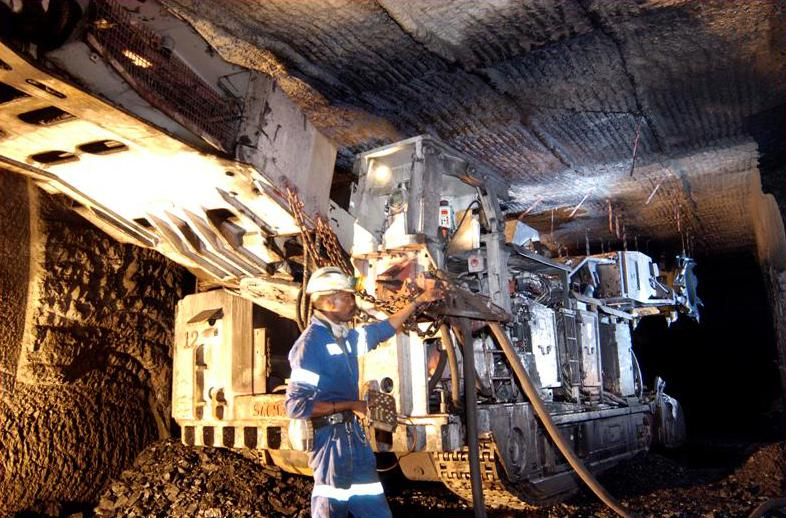
\includegraphics[width=0.7\textwidth]{Continuous_Miner.jpg}
\caption{Continous Miner. Pictured is the `Remote Continuous Miner HM21 Joy Used for underground coal mining',
 originally uploaded to Wikipedia by user Xlxgoggaxlx 
 under the Creative Commons Attribution-Share Alike 3.0 Unported license
 The machine operator must stand close to the machine and cutting interface to control the machine.
The operators use many cues, but ultimately must track if they are cutting the target material and 
the state of tool wear. Allowing operators to maintain a greater distance while giving them
the feedback they require can improve production and safety.
Image Source/License: \url{https://commons.wikimedia.org/wiki/File:Continuous_Miner.jpg}
}
\label{fig:conminer}
\end{figure}

The technologies proposed in this dissertation could be used to automate feedback collection
during the rock cutting process, allowing operators to perform their duties from a safer location.
This work investigates using measured frequency responses to predict material and wear conditions
using a non-linear dynamic capacitive load cell. 
An acoustic tool wear detection method is also developed using this same premise.
The capstone of this project is a custom capacitive load cell that is able to measure 
rock cutting forces using a linear model. 
Each of these three works are respectively summarized in the included journal articles.

This work was sponsored by NIOSH contract 75D30119C05413.
It is a continuation of prior work at Colorado School of Mines \cite{11124/170545}.
The previous work employed pieozo electric sensors to make measurements to estimate
rock cutting parameters. 
Our work focuses on use of a capacitive based load cell.
Study of rock fracture mechanics \cite{11124/14359} 
and the effects of tool geometry during rock cutting \cite{11124/13192, 11124/16423, 11124/176345} 
have long been pursued to increase mine efficiency and safety.
By providing an \textit{in-situ} force sensor, this work provides a means
for direct measurement of rock cutting parameters.
In addition to enabling operators to perform their roles from a distance,
this device could also be used to optimize tool geometries 
by providing quick and direct feedback of the cutting forces.

Safety in mines is a serious issue, and the next chapter discusses its current state.
The chapter after that covers additional background information regarding sensor choices.
Another chapter is then given which discusses modeling of the chosen sensors and materials.
The journal articles that summarize the work are included next. 
Each article describes the implemented classification or regression methods specific to the topic.
After the articles, a chapter which compares the different capacitive sensor implentations is given.
An additional chapter describing extensions of the acoustic processing methods is given after that.
This dissertation and the constituient articles have been published as 
Open Access and are released into the public domain.
If you would like implementation advice, you can contact me, the author, at:
austinfoltmanns at gmail dot com with the subject line containing "THESIS".
I hope you find this dissertation useful.


\chapter{
Mining Safety Background
\label{chap:2}}

In the thesis by Moore \cite{11124/16423}, the author outlines history of mining tools
dating back to the 1600s. This is when blasting was introduced to the mining process.
Hand tools dominated until the invention of steam powered machines in the mid 1800s.
Around 100 years later, at the time of publication of the thesis, compressed air hammer drills
were the most popular implement. These techniques and the mining drill bits that they used
evolved with each other over time.

The introduction of the continous mining machine increased productivity and 
was generally regarded as safe since the operator was enclosed in a shielded cab.
Around the 1980s, the remote control for the continous mining machine led to 
further increases in productivity, but with differing results for safety \cite{KONONOV199521}.
The remote control provides the operator greater visibility of the operation, 
but at increased risk of injury from the machine or tunnel collapse.
The crush hazards from the machine were not mitigated until the introduction of the
personelle proximity detector, around the turn of the milenium.
The detector prevents the machine from advancing into 
workers which are wearing the device \cite{schiffbauer2001active}.

Safety in underground coal mines has not improved over that last decade.
Statistics from 2011 to 2022, shown in \ref{tab:deaths},
show that coal mining has remained a dangerous industry,
especcialy for underground coal mine operators.
Mine technology has been the subject of extensive review 
\cite{ijerph19042334, 7784796, RALSTON2014305, molaei:hal-02940030}.
Different areas of research include process control and hazard detection.
Process control improvements can avoid hazardous conditions from being created,
making them proactive rather than reactive.

\begin{table}[]
\centering
\caption{Selected statistics from \url{cdc.gov/NIOSH-Mining/MMWC/}. Accessed April 14th, 2024}
\label{tab:deaths}
\begin{tabular}{|l|l|l|l|l|}
\hline
Year & Coal Injury Rate & All Injury Rate & Underground Coal Mine & All Mining Deaths \\
     & (Per 100 FTE)    & (Per 100 FTE)   & Operator Deaths       & (Coal included)   \\ \hline
2011 & 2.49             & 1.94            & 9                     & 37                \\ \hline
2012 & 2.40             & 1.86            & 12                    & 35                \\ \hline
2013 & 2.42             & 1.82            & 14                    & 41                \\ \hline
2014 & 2.48             & 1.83            & 10                    & 43                \\ \hline
2015 & 2.33             & 1.70            & 8                     & 26                \\ \hline
2016 & 2.40             & 1.64            & 7                     & 24                \\ \hline
2017 & 2.56             & 1.64            & 8                     & 27                \\ \hline
2018 & 2.22             & 1.52            & 6                     & 27                \\ \hline
2019 & 2.23             & 1.53            & 7                     & 27                \\ \hline
2020 & 2.30             & 1.42            & 3                     & 29                \\ \hline
2021 & 2.37             & 1.49            & 6                     & 37                \\ \hline
2022 & 2.24             & 1.42            & 6                     & 29                \\ \hline
\end{tabular}
\end{table}

In the cited reviews, examples of sensors in mining include
gas detectors, tunnel mapping, personelle detection, material composition measurement and more.
In the work by Ralston \cite{RALSTON2014305}, goals for autonomous mining systems are outlined in stages
from local manual control to full automation.
Current remote controls allow operators more mobility during cutting, and addition of 
more process feedback can allow them to be further from the cutting interface.
The sensor developed in this work could allow operators to perform tele-operation or tele-supervision,
whereby they are providing higher level commands to the machine using remote sensors for feedback, 
possibly augmented with feedback collected with their own senses.

Previous efforts to improve safety and efficiency have tried automating the continous mining process,
but fell short on being able to totally take over for human operators \cite{11124/170545, schiffbauer1988testbed}. 
Experienced operators are an invaluable resource. 
They have expert knowledge gained through years of working in difficult conditions,
frequently putting themselves in hazardous locations to collect the feedback they need.
Augmenting their expertise with objective feedback and allowing them to stay at a safer distance
stands to improve outcomes beyond fully human or fully autonomous control.

When working in an underground coal mine, machine operators must stand close to the cutting interface
and the machine to collect feedback to operate the machine. This places them at risk of being crushed 
by the machine or otherwise injured due to hazardous tunnel conditions.
Operators with long term careers are inevitably injured from the loud noises and harmful dust in the environment.
As long as this type of operation remains economically viable, it is likely to continue.

Improving both safety and efficiency is the optimal path for new technologies in an underground mine \cite{Sider1983}.
Mining safety has improved gradually over time and could currently 
be improved by moving operators further from the cutting interface.
Efficiency can be improved by implementing autonomous process control and feedback mechanisms.
for optimizing tool change scheduling and cutting control.
To enable these outcomes, we seek feedback mechanisms which can determine quantities of interest for the process.
The next chapter discusses sensor technologies that were considered for 
determining tool wear, material type, and cutting forces in underground coal mining.


\chapter{Sensors Technology Literature Review\label{chap:3}}

For this iteration of the smart bit project, many different sensing technolgies were considered.
Rock cutting tools are consumed quickly during underground mining, and need replaced frequently
to maintain cutting efficiency. 
Sensors at the cutting interface must be low power, low cost, and robust 
to be sucessful in the underground mine.
A table of different sensing technologies and requirements is shown in ~\ref{tab:sense_review}
Each sensing technolgy has different pros and cons, and are discussed in the following subsections.


\begin{table}[]
\centering
\caption{Summary of technology review, `X' indicates requirement is met.}
\label{tab:sense_review}
\begin{tabular}{|l|l|l|l|l|}
\hline
Sensor        & Robust & Low Cost & Low Power & Used Here \\ \hline
IMU           &        & X        &           &           \\ \hline
Custom MEMs   &        &          & X         &           \\ \hline
Photo         &        &          &           &           \\ \hline
Piezo         &        & X        & X         &           \\ \hline
Radio Antenna &        & X        & X         &           \\ \hline
Thermal       & X      & X        & X         &           \\ \hline
Strain Gauge  &        & X        &           & X         \\ \hline
Acoustic      &        & X        & X         & X         \\ \hline
Capacitive    & X      & X        & X         & X         \\ \hline
\end{tabular}
\end{table}

\subsection{IMU}

\subsection{Custom MEMs}

\subsection{Photo}

\subsection{Piezo}

\subsection{Radio Antenna}

\subsection{Thermal}

\subsection{Strain gauges}

\subsection{Acoustic}

\subsection{Capacitive}




\chapter{Method Selection}

Motivated by the selection of thin film polyimide sensors, 
models for their deformation were studied for this work.
The deformation of polyimide is linear for thick films
and small deformations, but for thin films, 
on the mesoscale of hundreds of micrometers,
polyimide films have nonlinear deformation.
These characteristics are manifested as creep, hysteresis, 
and temperature dependence.

Thin film deformation can be modeled using viscous elements, as shown in \ref{fig:sense_model}.
This is only an approximation, and depending on how nonlinear the dielectric deformation response is,
this model might not accurately capture the dynamics of the system.
The system overall is nonlinear, and with a material this viscous,
cycling the film rapidly will result in changes to the vibrational modes.

% Spring figure 
\begin{figure}[t]
    \centering
    \begin{circuitikz}
    \coordinate (A) at (-3.5, 0);
    \coordinate (B) at (-3.5, -2);
    \coordinate (C) at (0, 0);
    \coordinate (D) at (0, -2);
    \draw (A) to[spring] (B) ; 
    \node [right=4pt] at (-3.5, -1) {$K_{walls}$} ; % wall 1 spring
%    \draw (C) to[spring] (D) ; 
%    \node [right=4pt] at (3.0, -1) {$K_{w2}$} ; % wall 2 spring
    \draw (-1.80,-1.85) rectangle (1.8,-0.15);
    \draw (-1,-0.15) to[spring] (-1,-1.85) ;
    \draw (-0.15,-0.15) to[spring] (-0.15,-1.05) ;
    \draw (-0.15, -1.85) to[damper] (-0.15,-1.05) ;
    \node [right=8pt] at (0.15, -0.85) {\huge$\dots$};
    \node [right=4pt] at (1.00, -1.55) {$K_{p}$} ;  % polyimide spring
    \draw (0,0) to[short] (0, -0.15);
    \draw (0,-1.85) to[short] (0, -2);
    \draw (A) to[short] (C) ; % top bar
    \draw (B) to[short] (D) ; % bottom bar
    \draw (-1.2,-2) to[spring] (-1.2,-4) ; % bottom spring
    \node [right=4pt] at (-1.1, -3) {$K_{bottom}$} ;
    \draw (-1.2,0) to[spring] (-1.2,2) ; % top spring
    \node [right=4pt] at (-1.1, 1) {$K_{top}$} ;
    \draw [line width=0.5mm] (-3.2,-4) to (0.8,-4);
    \foreach \i in {-2,...,6} {
      \draw [line width=0.25mm] (\i/5 * 2- 2.1,-4) to (\i/5 * 2 - 1.6, -4.45);
    }
    \draw [line width=0.5mm] (-3.2,2) to (0.8,2);
    \draw [->] (-3,2) -- (-3,1.5) node [left] {$f(t)$};
    \end{circuitikz}
    \caption{A model of the sensor as a system of springs and dampers. 
             The PI can be modeled with a general visco-elastic model with
             repeating Maxwell elements. Here, it is summarized as $K_p$. 
             The springs representing the steel case top and bottom, $K_{top}$ and
             $K_{bottom}$, are much stiffer than the midsection. 
             Similarly, $K_{walls}$, of the steel case, is much stiffer than $K_p$.
             Thus the total device stiffness is readily approximated by 
             the stiffness of the device walls.}
    \label{fig:sense_model}
\end{figure}

The stackup for the sensor membrane for the first iteration of the capacitive load cell
is shown in \ref{fig:stackupsense}. This model had a very thin inner layer, which resulted
in nonlinear dynamics. The next iteration of the sensor uses a thicker membrane,
which results in a more linear sensor. 
The non-linearity of the first design was not an issue for tool wear or material classification,
but did impede using the measurements for force measurements. 
The next iteration of the design improved the sensor linearity.

% Stackup fig
\begin{figure}[t]
\centering
\begin{tikzpicture}
    \node[anchor=south west, inner sep=0] (image) at (0,0) 
      {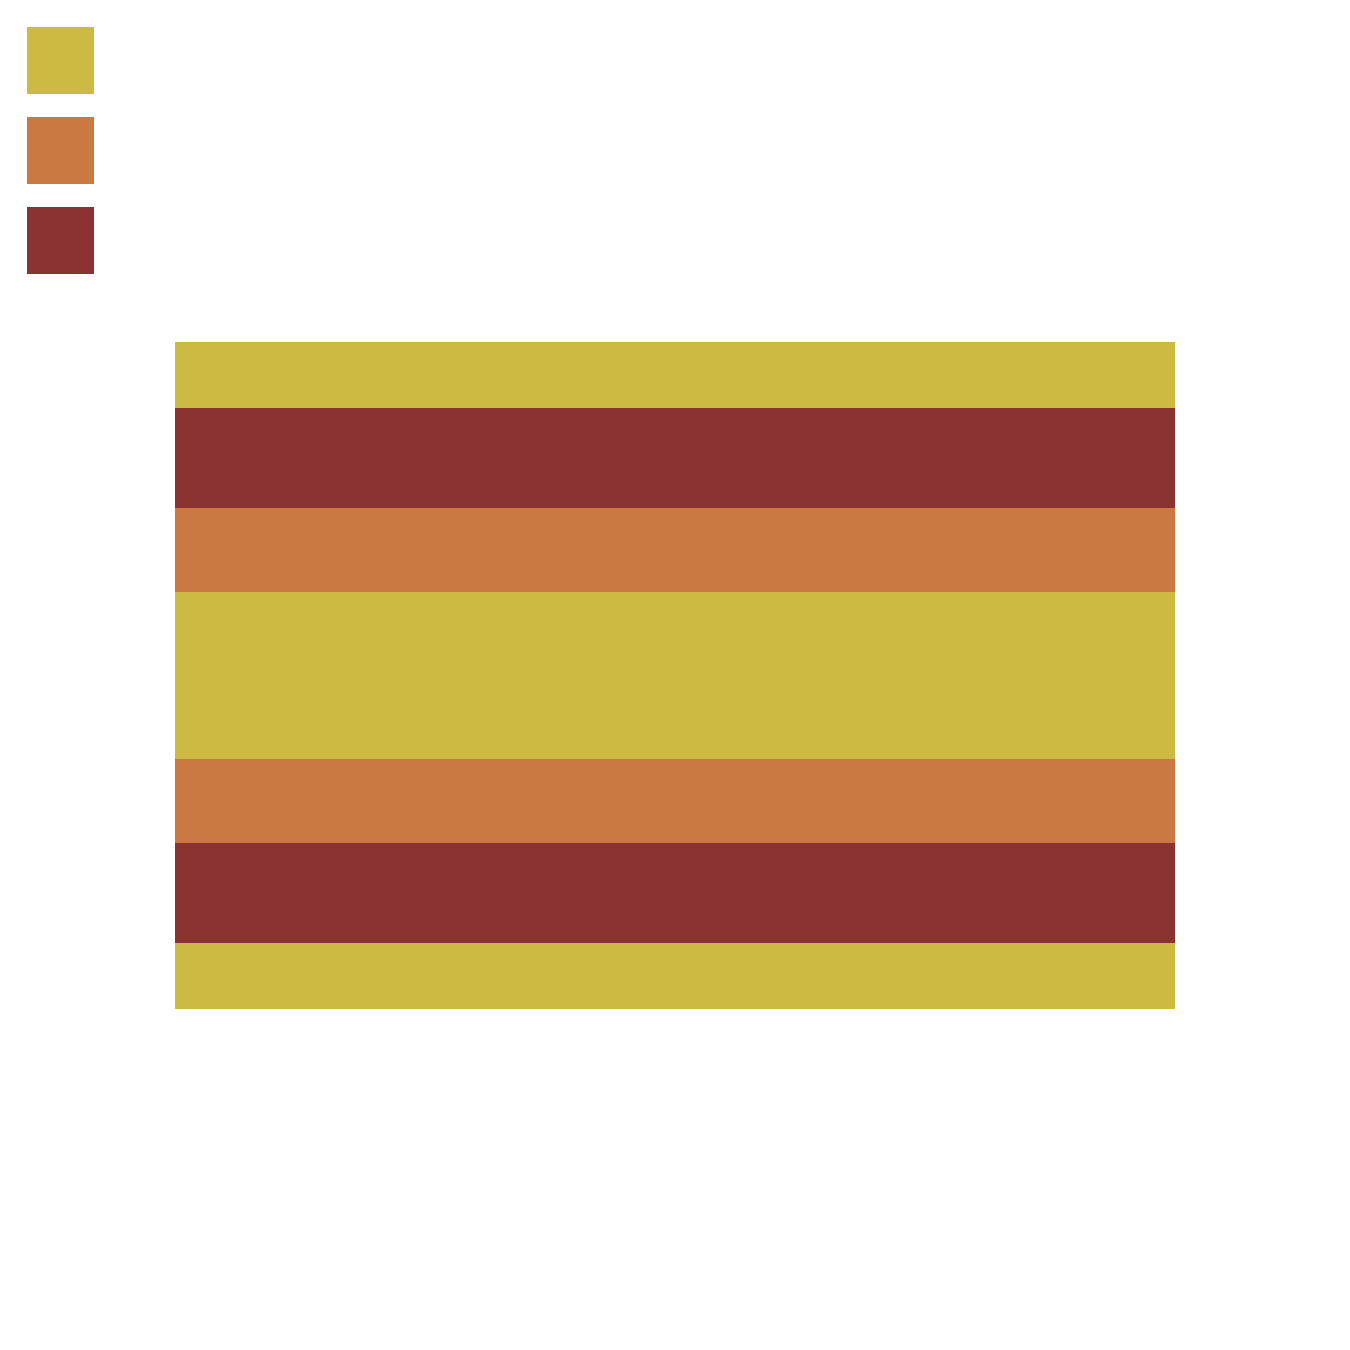
\includegraphics[trim=0 75 0 0,clip,width=0.55\linewidth]{figures/sensestackupxcf.png}};
    \begin{scope}[x={(image.south east)}, y={(image.north west)}]
      \node[anchor=west] at (0.08, 0.93) {Polyimide};
      \node[anchor=west] at (0.08, 0.845) {Copper};
      \node[anchor=west] at (0.08, 0.76) {Adhesive};
      \dimline {(0, 0.02)} {(0, 0.67)} {$100\mu$m};
%      \dimline {(1, 0.2)} {(1, 0.4)} {$d100\mu$m};
      \dimline[extension start length=-.50, extension end length=-.50]
                           {(.95, .28)} {(.95, .43)} {\small $25\mu$m};
      \dimline[extension start length=-1.500, extension end length=-1.500]
                           {(1, .43)} {(1, .51)} {\small $12\mu$m};
      \dimline[extension start length=-1.500, extension end length=-1.500]
                           {(.95, .61)} {(.95, .67)} {\small $12.5\mu$m};
      \dimline[extension start length=-1.500, extension end length=-1.500]
                           {(1, .10)} {(1, .18)} {\small $15\mu$m};
    \end{scope}
\end{tikzpicture}
\caption{The stackup for the FlexPCB sensing membrane. The outer PI layers are 12.5 $\mu$m
tall while the inner layer is 25 $\mu$m. The adhesive layers are 15 $\mu$m and the copper
layers are 12 $\mu$m. The total membrane height is about 100 $\mu$m. Due to the very thin
thickness of the dielectric film, the deformation characteristics will be dominated
by the interaction of the complex molecular chains and are expected to be nonlinear.
}
\label{fig:stackupsense}
\end{figure}

Other items which govern the vibrational forces during cutting include
the material type and the tool wear. 
Different rock types have different fracture mechanics, 
and these differences can be measured and classified.
Different tool wear levels require different amounts of cutting force,
and will result in changing fracture mechanics dependent of the tool's geometry.

All of these changes in vibrational modes and forces can be tracked in the
frequency domain as changes to the emitted spectra. For this research,
it is known that energy is moving from certain vibrational
modes to other vibrational modes across the categories of material type
and tool wear. This shift in energy over the spectra can be measured
by using the magnitude of the Fourier transform coefficients for a 
short duration sample.

As the Fourier spectra magnitude coefficients change, these changes 
can be used to classify the conditions that caused them.
We use data-driven classification techniques to identify these differences and 
predict the cutting conditions.
Doing so with a capacitive sensor and an acoustic sensor
is discussed in \ref{chap:P1} and \ref{chap:P2}, respectively.
Additional transforms and variations of the technique are discussed in \ref{chap:9}.
\ref{chap:P3} discusses the development of the sensor with more linear performance, 
while \ref{chap:8} compares the different capacitive load cell designs for this project.
The last chapter, \ref{chap:10} describes the fit of the linear model and 
further characterization data.



\chapter[
Capacitive Load Cells to 
 Promote Worker Safety
]{
Low-Profile Capacitive Load Cells for 
 Underground Mining Material and Wear Classification
 to Promote Worker Safety
\label{chap:P1}
}

\newcommand{\ora}{\overrightarrow}

\begin{center}
\bfseries{License:} Creative Commons licence CC BY: This licence allows readers to copy, distribute and transmit the Article as
long as it is attributed back to the author. Readers are permitted to alter, transform or build upon the Article,
and to use the Article for commercial purposes. Please read the full licence for further details at -
http://creativecommons.org/licenses/by/4.0/
\end{center}

\subsection{Abstract}

This work proposes a capacitive load cell for conical picks to enable 
 underground continuous mining machine operators to 
 perform their roles away from known hazardous regions near the machine.
The load cell is embedded in commercially available flexible printed circuit board,
 integrates with the target tooling, and demonstrates in-situ force sensing 
 of vibration signatures for continuous mining cutting tools.
Changes in material constitution, tool mass, and tool geometry cause modal variations
 in vibrational response measurable with force sensors at the cutting interface.
Time-series measurements are captured during rock cutting tests using a linear cutting machine.
These measurements are segmented into small windows, less than 0.25 seconds, and are preprocessed 
 using the fast Fourier transform, which highlights the modal variations.
The transformed measurements are then classified into different material and wear categories
 using support-vector machines with the radial basis function kernel.
Different normalization schemes and Fourier transform methods are tested for signal preprocessing.
Results show that the power spectral density measurements with normally distributed coefficients 
 give good results for material classification, while the normalized time-domain measurements
 give better results for wear classification.
Under laboratory conditions, this technique is shown to 
 classify material and wear categories with F1 score above 0.85 out of 1.0 for our experiment.
This technology could be used to assist operators in assessing material and wear conditions from
 a safer distance. 
It has applications in the coal mining industry as well as other applications
which use conical picks such as road milling.

\subsection{Introduction}\label{sec1}

Operators monitoring important process feedback in hazardous regions is dangerous \cite{jobes12}.
Operators are expected to monitor machine alignment, tool wear, machine condition, and the material being cut \cite{sanders81}.
The hazards that the operators are exposed to in underground mining can be difficult to model \cite{JiangYaodong2017Arom}.
To allow operators to perform their role from a greater distance, 
 we propose a sensor suitable for assisting operators in assessing material type and tool wear that integrates
 with conical picks on continuous miners used in underground coal mining.

Underground mining is dangerous and safety has not been improved over the last decade, 
 with fatalities per 100,000 full time equivalent employees averaging 21.4 from 2011-2020 \cite{nioshdata}.
In particular, coal workers are roughly 50\%
 more likely to be injured than workers in other mining sectors and
 account for roughly 50\% of fatalities from 1983 to 2020\cite{nioshdata}.
Existing technologies for mitigating these hazards monitor the environment 
 with micro-seismic sensors, distributed pressure sensors, or electromagnetic analysis \cite{JiangYaodong2017Arom}.
These technologies only identify hazards after they occur. 
Elimination of hazardous conditions is the most effective method for reducing risk to workers in any application \cite{niosh_2015}.
The only way to eliminate these hazardous conditions is to allow the operators to perform their role from a greater distance.

Previous efforts to allow operators to perform their role from a greater distance,
 namely development of remote controls, have allowed operators to 
 collect better visual feedback; however, 
 operators often put themselves in hazardous positions to do so \cite{bartels09}.
Technologies also assist operators by automating some tasks. 
For example, automated hydraulic diagnostic systems can help operators 
 monitor the machine's hydraulic conditions \cite{mitchell91}.
One of the most effective technologies for reducing worker injury is the personnel proximity detector, 
 which disables certain machine operations if designated zones near the machine are entered 
 by persons tracked with the device \cite{bissert16}. 
This device was implemented about a decade ago; however, there have not been 
 any major improvements since.

Direct measurements of rock and pick interaction have previously noted 
 significant differences in forces between tool wear levels \cite{sundae85, donna90}.
Material has been differentiated by vibration signatures using various classification techniques
 as early as 1993 \cite{gary93}.
Previous efforts for smart bit or intelligent pick tooling to perform these tasks in real-time during operation 
 have taken place over the last few decades, examples include:
 using neural networks to classify tool wear in potash \cite{potashMeyersThesis}, 
 using acoustic data to classify both material and tool wear in coal cutting \cite{shen1996acoustic}, 
 using piezo sensors to deduce rock chipping \cite{smartbitMillerThesis},
 and, most recently, using an instrumented block with integrated strain gauges to measure cutting forces \cite{fries21}.
So far, results using capacitive load cells have not been found for 
 material and tool wear classification in underground mining. 
Advances in both capacitive sensing and vibration classification 
 have unearthed a variety of applications in other domains.
Our sensor, shown in \ref{fig:senseonpick}, can assist operators in assessing material type and tool wear
 by measuring differences in vibrational responses between the different conditions.


\begin{figure}[t!]
\centering
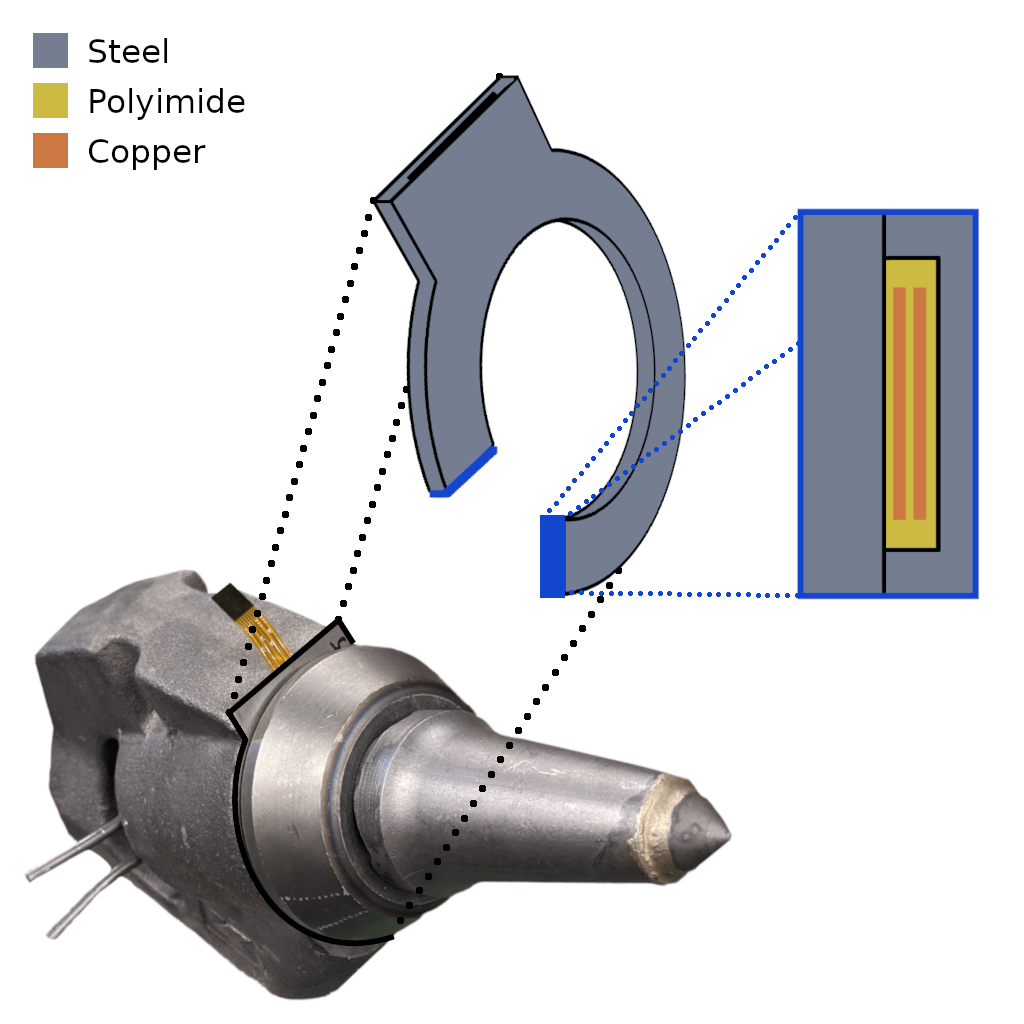
\includegraphics[width=3in]{figures/p1_media/Fig1.png}
\caption{A prototype of the sensor integrated with the U92 4.0 22NB  Conical Pick
 and K35 Block system, from Kennametal. The device is shown without the measurement
 collection system and is situated between the sleeve and the block.
The FlexPCB interface is exposed, which provides access to the capacitive sensors' electrodes.
 A steel case protects the FlexPCB sensor and
provides the necessary stiffness to transfer the input forces to the sensor.
An embedded electronics platform, not shown in this figure, takes measurements
 suitable for dynamic classification of tool-wear and material. 
A cutaway of the sensor shows the thin film design for the force sensor.}
\label{fig:senseonpick}
\end{figure}


To test our sensor for material and wear classification, full-scale rock cutting experiments are 
 performed using the linear cutting machine at Colorado School of Mines,
 a popular type of tool for rock cutting mechanics testing \cite{rostami21}.
A limestone sample cast in concrete is used to test material classification. 
Conical picks of three different wear levels at an attack angle of 45 degrees are used for tool wear classification.
The wear levels are \textit{new}, \textit{moderate}, and \textit{worn}, where \textit{moderate}
 represents a pick halfway through its useful life, and \textit{worn} is a tool at the end of its useful life.
The tool tips are artificially worn to a spherical diameter using a lathe 
 to approximate an even wear pattern and for reproducibility.
A closeup view of the tool tips and the values for their spherical diameters is shown in \ref{fig:tips}.
The low profile sensor sits between the sleeve and block.
The sleeve has been machined down to a slip fit in the block to allow force transfer to the sensor.
The sleeve and block are both retained by a large pin.
Measurements are collected from the sensor using an embedded capacitance to digital converter and sent to a 
 computer over USB.

\begin{figure}[t!]
\centering
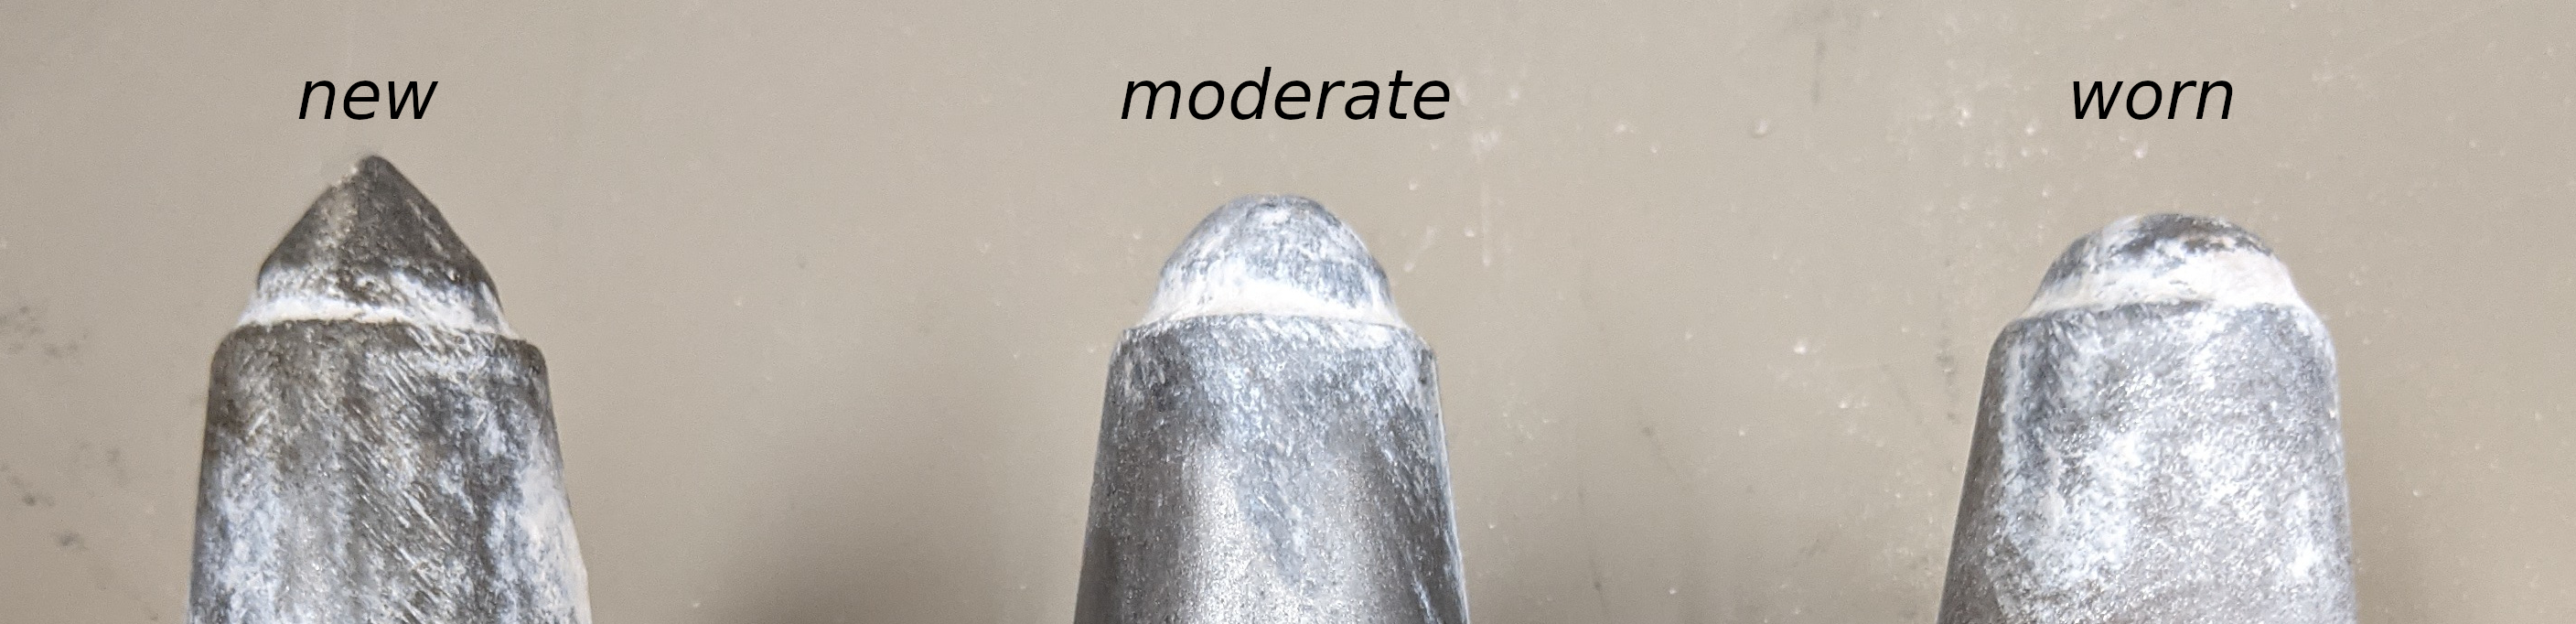
\includegraphics[width=3in]{figures/p1_media/Fig2.png}
\caption{The different pick wear levels. The \textit{new, moderate}, and \textit{worn}  pick tips
  have spherical diameters of 3.71 mm, 17.9 mm, and 27.5 mm respectively. 
 This approximates and even wear pattern. 
 The \textit{moderate} and \textit{worn} tips were artificially worn using a lathe.}
\label{fig:tips}
\end{figure}

To highlight the changes in vibrational modes, the data is transformed using
 short window fast Fourier transform preprocessing before classification.
The resulting vectors are classified into material and wear categories 
 using the support-vector machine technique. 
Data from strain gauges embedded in the linear cutting machine and our custom sensor are 
 both used on their own for classification.
Each classification system in our experiment is scored using 
 the F1 score \cite{sasaki2007truth, powers2020evaluation}.
The best performance for material and wear classification  
 yielded F1 scores around 0.85 out of 1.0 for our experiment.
Performance in tool wear classification is shown to be comparable between the custom sensor and the 
 strain gauges embedded on the linear cutting machine. For material classification, the additional
 sensitivity due to the proximity of the custom sensor to the cutting interface allows it to 
 perform better using the same algorithm.

The rest of this article is organized into sections. 
First, background information regarding material and wear classification algorithms is given along 
 with a description of the algorithm we use.
Then, the sensor design and characterization is described.
After, the procedure for the rock cutting experiment is given,
 followed by the performance results of the classification algorithm.
Finally, some discussion points and conclusions regarding the experiment and results are shared.


\subsection{Material and Wear Classification}
Material identification techniques for rock cutting can use metrics based in
 force and energy measurements, as different rock materials are known to require
 varying energy to break down \cite{teale65,klyuchnikov19}.
For tool wear classification, force or vibration feedback is commonly used in other domains such as 
 metal milling or oil drilling because changes in tool mass and geometry cause 
 the vibrational modes to shift \cite{klaic18, abu03, tao09, tao10}.
Both material and tool wear classification can be framed as a vibration classification problems.
Vibration classification lends itself towards certain standard
 signal processing and classification techniques,
 primarily with frequency domain preprocessing \cite{liu18}.

Preprocessing the input sensor data using different spectral or statistics
 based methods to improve classification results
 is popular \cite{peng11,tao09,qian10,tao10}.
For this research, the fast Fourier transform is chosen as the preprocessing technique
 as it has been shown to give good results in many domains \cite{ram09}.
Depending on the chosen kernel for the support-vector machine, data standardization
 can range from beneficial to necessary, as the kernel may be built with assumptions
 on data mean values and range.
The effects of the chosen normalization and preprocessing methods, 
 or their absence, on the classification results are explored in this work.
%For an overview of well-established spectral techniques and advice for higher
% order techniques, the reader is referred to \cite{niki87}.

The classification technique used after preprocessing is the support-vector machine (SVM)
 using the default `C-Support Vector Classification' implementation in the Python library
Scikit Learn \cite{chang11}, \cite{platt99}.
SVM has long been known to be able to classify model behaviors \cite{mukh97}.
It has also shown useful specifically in tool  monitoring \cite{sun04}.
In general, the SVM works by finding a hyperplane in the data set
 which separates the data into the prescribed categories
 then, this hyperplane can be used as a quick decision rule
 for classification of future inputs \cite{chang11}.
The advantage of the SVM is it first transforms
 the input data to a higher dimension using a kernel function which helps to separate the data.
This method has few hyperparameters and is considered
 generalizable, only needing relatively little training data to achieve good performance.

The SVM technique has few hyperparameters when compared to other 
 machine learning techniques like feed-forward or convolutional neural networks, 
 which allows it to be implemented quickly and be generalizable. 
The SVM is also typically better performing than simple techniques like k-nearest neighbors.
K-nearest neighbors is another popular and low hyperparameter technique
 for vibration classification, and it works by selecting the majority class
 of the `k' samples closest to the input in its memorized training data \cite{hu21}.
The SVM solves the classification problem in a similar way, but reduces the training data
 for computational efficiency and better sensitivity to general trends.
More advanced techniques, such as feed-forward or convolutional neural networks,
 are flexible techniques for vibration classification that work by numerically optimizing
 a series of weighted vector functions to approximate the statistical likelihood
 of a given input being from each output class based on the training data \cite{chen16}.
SVM strikes a balance between these techniques as it generally has better performance than k-nearest neighbors 
 but is not as prone to over-fitting as the feed-forward or convolutional neural network.

\subsubsection{Classification Methods}

Time-series measurements are recorded from the four channels of our custom sensor
 and the four channels of the strain gauges on the linear cutting machine.
For either sensor, we denote these measurements as $CH_x[n]$, where $x$ is the channel index 
 ranging from 1 to 4 and $n$ is the sample index ranging from 1 to $T$, the total number of measurements. 
These time-series measurements from each sensor are then chopped into small segments representing 
 short duration ($\leq 0.25$ s) windows of signal. 
These discrete vectors are preprocessed to form the feature 
 vectors to be classified by the support-vector machine. 
For an individual classification sample, the data from a particular
 channel can be denoted as $\ora{C_{kx}} = [CH_x[k], CH_x[k+1], \ldots, CH_x[k+M-1]]^\top$, where
 $k$ is the index corresponding to the start time of the sample window, $x$ is again the channel index,
 $M$ is the number of samples in the window, 
and $[\> \cdot \>]^\top$ represents the matrix transpose operation.

Both window overlap and window size are varied during our tests to observe their effects on performance. 
Increasing window overlap generates more data vectors for training and testing,
 but the resulting samples are more redundant than those generated with less overlap.
Increasing window size gives data with more features which can improve classification accuracy.
The classification rate is limited to one classification per window, 
 and windows may overlap to increase the rate.
A short window which gives acceptable performance is desired 
 for rapid classification suitable for real-time use. 

Each point in time can be assigned a class label for both material and wear. 
Only windows with contiguous labels are used in the experiment. 
Samples which are near the beginning or end of a material are discarded, 
 as they do not have a clear ground truth label and are not representative of the
 steady state cutting dynamics.
Separate classification systems are trained to identify material and wear.
For an individual classification experiment, the set of paired measurement and class data
 is split randomly into testing and training sets.
The set with the training indices is denoted in this work as $R$, while the set of testing indices is $Q$.
After being windowed and split, the feature vectors for classification via 
 support-vector machine are represented as:
\begin{align}
\ora{X_i} &= \mathcal{P}_{\theta} \Bigg( \begin{bmatrix}  \ora{C_{k1}} \\[1ex]
                              \ora{C_{k2}} \\[1ex]
                              \ora{C_{k3}} \\[1ex]
                              \ora{C_{k4}} \end{bmatrix} \Bigg) ,
\end{align}
were $\mathcal{P}$ is the preprocessing pipeline for the data and $\theta$ are the parameters fit from the
 samples in the training set.
The subscript, $i$, is the sample index and ranges from 1 to $N$, the total number of vectors
 in the data set. The specific mapping between $i$ and $k$ depends on the window parameters.
The Scikit `sklearn' library \cite{chang11, platt99} provides a convenient data structure, the Pipeline object, 
 which encapsulates these steps for consistent application and ensures that data from the 
 testing set is not used during parameter fitting. 

\begin{table}[h]
\centering
\caption{Preprocessing Pipeline Steps, $\|\cdot\|, \cdot^2$, and $\sqrt{\cdot}$ are element-wise
 absolute value, square, and square root respectively.}
\label{tab:preproc}
{\renewcommand{\arraystretch}{1.5}%
\begin{tabular}{l|l|l}
Symbol                  & Values         & Description    \\ \hline 
\multirow{2}{*}{$\mathcal{N}_\theta^1, \mathcal{N}_\theta^2$} & StandardScaler 
   & $\mathcal{N}(\ora{X_i}) = \big(\ora{X_i} - \underset{i \in R}{\mathrm{mean}} (\ora{X_{i}}) \big)/ 
                                  \underset{i \in R}{\mathrm{std}}(\ora{X_{i}})$ \\
   & None/Control   & $\mathcal{N}(\ora{X_i}) = \ora{X_i}$   \\ \hline
\multirow{3}{*}{$\mathcal{F}$}      & FFTMag        
              & $\mathcal{F}(\ora{X_i}) = [\|FFT(\ora{C_{k1}})\|,  ..., \|FFT(\ora{C_{k4}})\|]^\top$     \\
              & FFTSQ        & $\mathcal{F}(\ora{X_i}) = [FFTMag(\ora{X_i})]^2 $         \\
              & FFTSQRT       & $\mathcal{F}(\ora{X_i}) = \sqrt{FFTMag(\ora{X_i})}$      \\
              & None/Control  & $\mathcal{F}(\ora{X_i}) = \ora{X_i}$           
\end{tabular}}
\end{table}

For our experiment, the pipeline consists of the composition of three optional operations, 
 detailed in \ref{tab:preproc}, and discussed here:
\begin{align}
\mathcal{P}_\theta &= \mathcal{N}_\theta^2 \circ \mathcal{F} \circ \mathcal{N}_\theta^1
\end{align}
where $\circ$ represents the function composition operator.
The steps denoted with $\mathcal{N}$ are normalization steps which transform the input
 data to be zero mean and unit variance along each feature using the sample mean and variance
 from the training set. 
The $\mathcal{F}$ operation is the frequency based transform, and different variations of 
 the fast Fourier transform are used. 
Every combination of processing steps is used, 
 and the results are compared to determine the best methods for this application. 
Each step is also substituted with the identity function during this process as a control.

In addition to the preprocessing step, the support-vector machine also can apply a transform to the 
input data during its use. A description of the support-vector machine algorithm, 
 adapted from \cite{smola2004tutorial} is given here.
Intuitively, the support-vector machine finds a hyperplane between two sets of data. This 
is done efficiently by representing the hyperplane as a linear combination of a subset of the 
training data. These vectors from the training data are known as the support vectors.
The binary classification support-vector machine works by solving the primal problem:
\begin{align}
\min_{w, b, \xi} \quad & \frac{1}{2} \|w\| + C \sum_{i\in R} \xi_i, \\
\mathrm{s.t.} \quad & y_i [w^\top \phi(\ora{X_i}) + b] \geq 1 - \xi_i, \quad \forall i \in R.\\
                 & \xi_i \geq 0, \quad \forall i \in R.
\end{align}
where $w$ and $b$ are the vector and offset representing the decision boundary hyperplane,
$\xi_i$ are slack variables which allow for error in classification in case of an infeasible problem.
The $y_i$ are binary class labels with value -1 or 1, $C$ is a regularization parameter, 
and $\phi(\cdot)$ is an implicit function which transforms the feature vectors into a higher dimension
before separation with the hyperplane. The function $\phi(\cdot)$ is implicit because in practice 
the dual of the primal problem is solved and only the inner product of the transformed input vectors 
is computed. This is done with the `kernel trick', whereby a kernel function, $K(x,y)=<\phi(x), \phi(y)>$
is used, which is less costly to compute than the full inner product in the higher dimension. After solving
the dual problem, the decision function for an unseen sample, $\mathbf{x}$ is given by:
\begin{align}
y_{pred}(\mathbf{x}) = \mathrm{sgn} \bigg( \sum_{i \in S} \alpha_i y_i K(\ora{X_i}, \mathbf{x}) + b \bigg),
\end{align}
where the $\alpha_i$ are the new coefficients given from the dual formulation 
 and $S$ is the set of support-vector indices. 
It is noteworthy that the final decision function does not explicitly use the hyperplane
 as represented by $w$, but instead relies the offset variable $b$ 
 and dot products (through the kernel) with the training data.
To use the support-vector machine for multi-class problems, the chosen implementation
 uses a `one-vs-one' voting scheme where a binary classifier is trained for each pair of
 class combinations. The class with the lowest index and most votes is chosen as the output.

The radial basis function is a popular kernel choice, as it was one of the first to be developed.
It is similar in function and performance to using auto-correlation as the 
 implicit function \cite{kong2007autocorrelation}.
Since the radial basis function gave acceptable performance 
 and to limit the number of hyperparameters, only it is used for this study.

To test our classification system, the feature vectors are sorted into testing and training sets
using ratios of 25:75, 50:50, 75:25. Each split is done randomly, 100 times, for each combination of
preprocessing parameters. Hyperparameters for our method are window duration, window overlap ratio, and window shape.
Window duration is set to 0.05, 0.10, 0.15, 0.20 and 0.25 seconds, 
 while overlap ratio is set to 0.25, 0.50, and 0.75. 
The window shape is left as rectangular for the entire study.
Ringing effects from frequency convolution with the $\mathrm{sinc}(\cdot)$ shape of the window in the
 frequency domain will be applied consistency across samples.
Discovery of the optimal window shape would require it's own extensive hyperparameter study
 across the many popular window functions. 
To limit the scope of the study, and since adequate performance was given with the rectangular window,
 focus is given to the other hyperparameters.

The effect of the preprocessing steps or their absence is investigated for this classification system
 across the hyperparameters of window size and overlap.
Each classification setup is scored using the F1 score \cite{sasaki2007truth, powers2020evaluation} 
 which is the harmonic mean of the classifiers precision and recall:
\begin{align}
F_1 &= 2 \frac{\mathrm{precision} \cdot \mathrm{recall}}{\mathrm{precision} + \mathrm{recall}}
\end{align}
Precision is the ratio of positive classifications that are correct while recall is the ratio of 
 positive samples which are correctly identified \cite{powers2020evaluation}.
The F1 score provides a numeric value between zero and one, with one being a perfect score. 
For our multi-class problem, we train the SVM using the `balanced' strategy where classes 
 are given equal weight, regardless of class samples size, by setting regularization term, $C$,
 inversely proportional to the class frequency in the input data.
We score the classifier using `macro' averaging for the F1 score
 where the final score is the unweighted average of the F1 scores for each class.
Using this setup, the classifier is trained to give equal weight to each class type,
  regardless of population size, and classification 
 performance and is scored with a metric which also gives equal weight classifier performance
 for each class. Additionally, confusion matrices and accuracy measurements are 
 used to get a more complete sense of classifier performance.

From this study, the optimal subset of steps may be found in a verifiable way. The training and testing
 computations are performed on the Isengard supercomputer at Colorado School of Mines. Individual classifiers
can be trained on a consumer laptop in less than a minute, but to run the thousands of tests for this study
 in a batch manner, the supercomputer is more appropriate.
For each set of parameters, the mean and standard deviation of the F1 scores
 are recorded for a population of 100 experiments with different random splits of data.
Setups giving scores with large deviations or high dependence
 on the test and train ratio are suspect for overfitting to non-relevant features in the data set,
 while a low deviation with a high mean F1 score that is similar across test and train ratios can be 
 considered generalizable and useful for the target application.
To meaningfully compare distributions of scores generated for each method,
 the Welch-Satterthwaite method (Welch's t-test) is used to determine 
 if differences are significant \cite{tamhane2000statistics}

\subsubsection{Sensor Design Literature Review}
When it comes to designing a sensor for underground mining applications,
 there are several key constraints: the device must be low power, low cost,
 and highly durable. Capacitive sensors generally meet these requirements.
Sensors that are not considered directly for this study are Inertial Measurement Units (IMUs)
 or custom microelectromechanical systems (MEMS) devices due to their power consumption, cost, and fragility.
The most promising fabrication technology found during our literature review was
 capacitive load cells embedded in flexible printed circuit boards.
The sensor dynamics can be non-linear, so the collected measurements 
 are compared to those of a linear force sensor. 

Capacitive pressure sensor designs have used
 steel enclosures \cite{lee16}, film dielectric \cite{bodini18},
 and sensors made directly from flexible circuits \cite{lee08}.
Larger film dielectrics can be modeled with a general system of springs and dampers;
 however, with thin films only a few dozen $\mu$m thick, the molecular dynamics
 contribute greatly to the response \cite{willam02} and make it non-linear.
Encasing the flexible circuit element in an enclosure provides a rigid structure
 with more linear deformation, but the dielectric still affects the relationship
 between the input force and the measured capacitance.
These flexible sensors are low in cost,
 while sensors which provide more linear measurements normally employ careful
 manufacturing processes, air gap designs,
 and different signal processing techniques such as those seen in
\cite{barile19,Lu16,Zaitsev17,Prit19,Liu16}.
Sensors which use thin films with non-linear deformation must use appropriate models
 and algorithms to achieve the desired classification results.

Popular flexible dielectric materials like carbon-doped
 thermoplastic poly-urethane and silicone can exhibit non-linearity
 through hysteresis, viscoelastic effects, or measurement creep
 \cite{Shouten17,Wolter18,Dommelen20,Kisic19}.
The choice of dielectric material for a capacitive sensor will 
 influence much of its performance, so it is important that the material
 have robust properties for the expected range of conditions.
Polyimide %(also known as PI) 
is a notable flexible dielectric material and
 sensor substrate for capacitive sensors due to its high temperature range,
 solvent resistance, and low surface roughness \cite{Khan14}.
It is also easily integrated with electronic circuits boards, known as
 flexible printed circuit boards, where it serves as the substrate for conductive traces.
However, when used in a thin film, polyimide has nonlinear deformation dynamics due to the complex
 molecular interactions of the constituent polymer chains \cite{VALAVALA20071161}. 
This viscoelastic-plastic behavior can be difficult to model for a large range of input,
 with models either incorporating complicated numerical integration techniques
 \cite{dharmadasa20, li21},
 only capturing the linear viscoelastic portion for small ranges \cite{he16},
 or ignoring the unloading phase \cite{wang20}.
Thicker films generally have a greater linear range \cite{chang08} and most models
 incorporate some mix of viscoelastic and viscoplastic elements like the model seen
 in \cite{wei08}.

Other works which have used polyimide as the force or pressure sensor
 dielectric show mixed results for sensor performance.
In one study, electrospun polyimide nanofibers were used as the
 dielectric to achieve measurement repeatability and sensitivity \cite{zhu20}.
When the device was cycled from 0 to 10 \% change in nominal capacitance for 10,000 cycles,
 no noticeable measurement creep was observed.
In another study, spin coated polyimide was used, and the sensor response was much noisier
 and subject to some initial transient effects \cite{dobrzynska12}.
Another group used a FlexPCB force sensor encased in polymeric materials and
 it showed good linearity and low hysteresis for 1\% changes in capacitance \cite{Bodini19}.
These studies indicate that polyimide is a good low-cost material choice that can still give
 good performance.


\subsubsection{Sensor Design}

To design a capacitive force sensor for material and wear classification, suitable choices must be made for
 materials, geometry, and the balance between sensor accuracy and bandwidth. 
Based on the sensor design literature review, 
 a steel case with a load cell embedded in a flexible polyimide circuit board is chosen for the design. 
The steel is 303 series stainless, chosen to reduce potential for corrosion and for its
 resistance to fatigue.
The steel case is made by chemical etching of 0.036 inch steel plates. 
A channel of 0.018 inch depth is formed on one plate and the two are laser welded together after
 a steel shim and the sensing membrane have been put in place.
As noted in the prior section, polyimide is chosen for the sensing membrane for its
 wide range of operating conditions and robust properties.
The sensor case geometry is largely determined by the target tooling, but must still be tuned to the operational
 requirements of the sensor. 
Likewise, the balance between sensor accuracy and bandwidth must be tuned to achieve the desired results.

To tune the case geometry for the desired stiffness, appropriate values must be chosen for the
 thickness and height of the side walls.
These values are shown as $\mathbf{h}, \mathbf{w_1}$ and $ \mathbf{w_2}$ in \ref{fig:sensecut}.
The donut shaped sensor has a center filled with viscous polyimide. 
The thickness and height of the side walls chiefly determines the spring constant of the sensor.
The polyimide is much more compliant than the surrounding steel, so the overall case deformation is not 
 influenced by its deformation in a significant way.
However, the capacitive cells are directly embedded in the polyimide, so the measurement is greatly 
 influenced by its deformation.


\begin{figure}[t!]
\centering
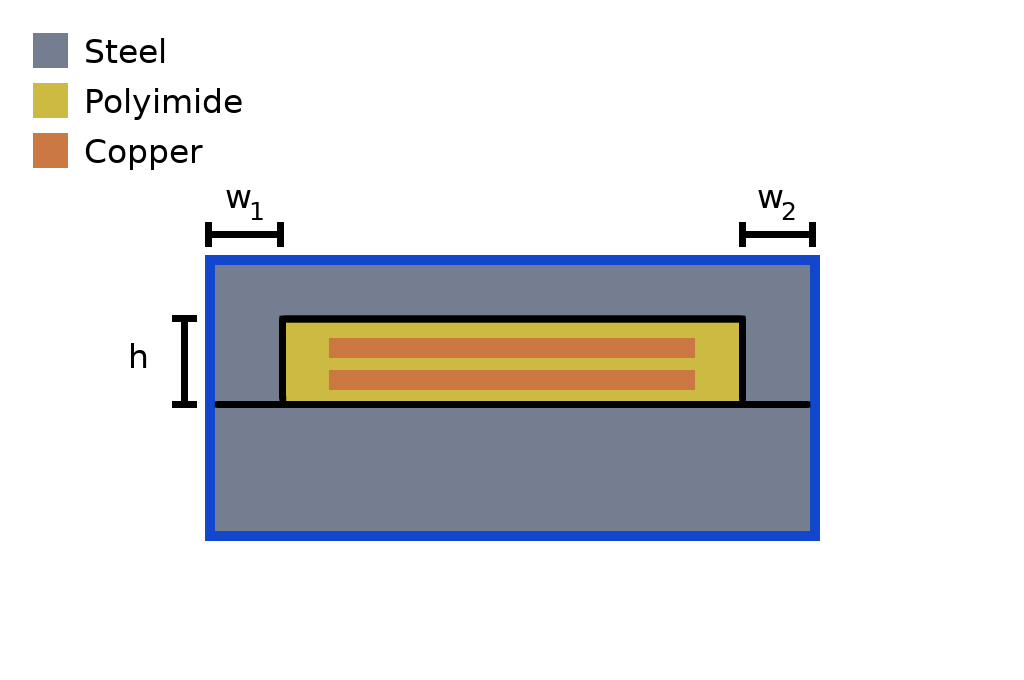
\includegraphics[width=3in]{figures/p1_media/Fig3.png}
% sensor geometry cutaway
\caption{
A cutaway of the sensor with the geometric parameters shown. The dimensions of the walls
 may be tuned to give the sensor the appropriate stiffness. The thickness of the top and bottom plates
 do not significantly influence the overall stiffness of the device.
}
\label{fig:sensecut}
\end{figure}


The sensor is designed for a maximum expected force of 200 kN. 
This provides some margin above the expected forces, which can be in excess of 100 kN for hard rocks.
The sensor case is tuned to have around 10\% strain at maximum load, in this way material fatigue can be 
 mitigated and the measured capacitance should be close to linear with dielectric deformation.
The thickness and height of the side walls, $\mathbf{h}, \mathbf{w_1}$ and $\mathbf{w_2}$
 are set to about two and a half millimeters.
The deformation of the steel case is expected to be mostly linear within this range of deformation.

The balance between sensor accuracy and bandwidth is determined by the range of deformation of the sensor
 as well as the capacitance and resonant frequency of the sensing circuit.
In general, larger capacitance values will provide greater accuracy at the cost of sensor bandwidth.
For the chosen hardware, the effective number of bits for the measurement 
 is proportional to the square of the measurement time. 
Larger capacitances take longer to settle but can make more accurate measurements.

Given the tool geometry, four cells are placed in the donut: two large and two small.
For our parallel plate design, it is important that the electrodes receive even loading,
 otherwise the parallel plate approximation is no longer valid.
The large cells are designed for a nominal capacitance of 541 pF and 
 the small cells are designed for a nominal capacitance of 412 pF.
All four pads occupy about $50^\circ$ and are spaced evenly around the donut.
The larger cells have about 30\% greater area.

Since we are focused on high-frequency vibration classification, 
 sensor bandwidth is maximized while still 
 providing sufficient resolution and accuracy for classification.
At a rate of 400 samples per channel per second, and using a gain of 4, 
 the embedded system is able to provide 128 levels for up to a 25\% change in capacitance.
At 10\% max expected deformation, the max expected change in capacitance is also about 10\%.
The true deformation of the polyimide around the electrodes is nonlinear and must be characterized to 
 make informed decisions with the resulting measurements.
 

\subsubsection{Sensor Characterization}

The sensor was characterized using load frame testing.
Five different load rates were applied to three separate sensors to achieve a max force of 200 kN 
 momentarily before ramping back down at an equal rate. 
Linear sensors show symmetric behavior for such a test, 
 but the sensor measurements for this test, shown in \ref{fig:triangleload}, 
 reveal that our sensor exhibits hysteresis and rate dependence for these loads.
These effects can be expected from the previous literature regarding polyimide deformation
\cite{Khan14, VALAVALA20071161, dharmadasa20, li21, he16, wang20, chang08, wei08, zhu20, dobrzynska12, Bodini19},
 and they obscure the effect of the average force on the measurement.
It can be seen that, as the loading rate increases, the traces converge.
This implies that the sensor can still be used to detect the changes in the high frequency components 
 of the response that are useful for vibration classification.
The overall deformation of the sensor case during these same loads is shown in \ref{fig:casedeformation},
 and the deformation is linear. 
This confirms that the nonlinear deformation is happening in the polyimide
 and suggests that this case could be used to house other sensing technologies
 that can transduce displacement to electrical signals.

\begin{figure}[t!]
\centering
\centerline{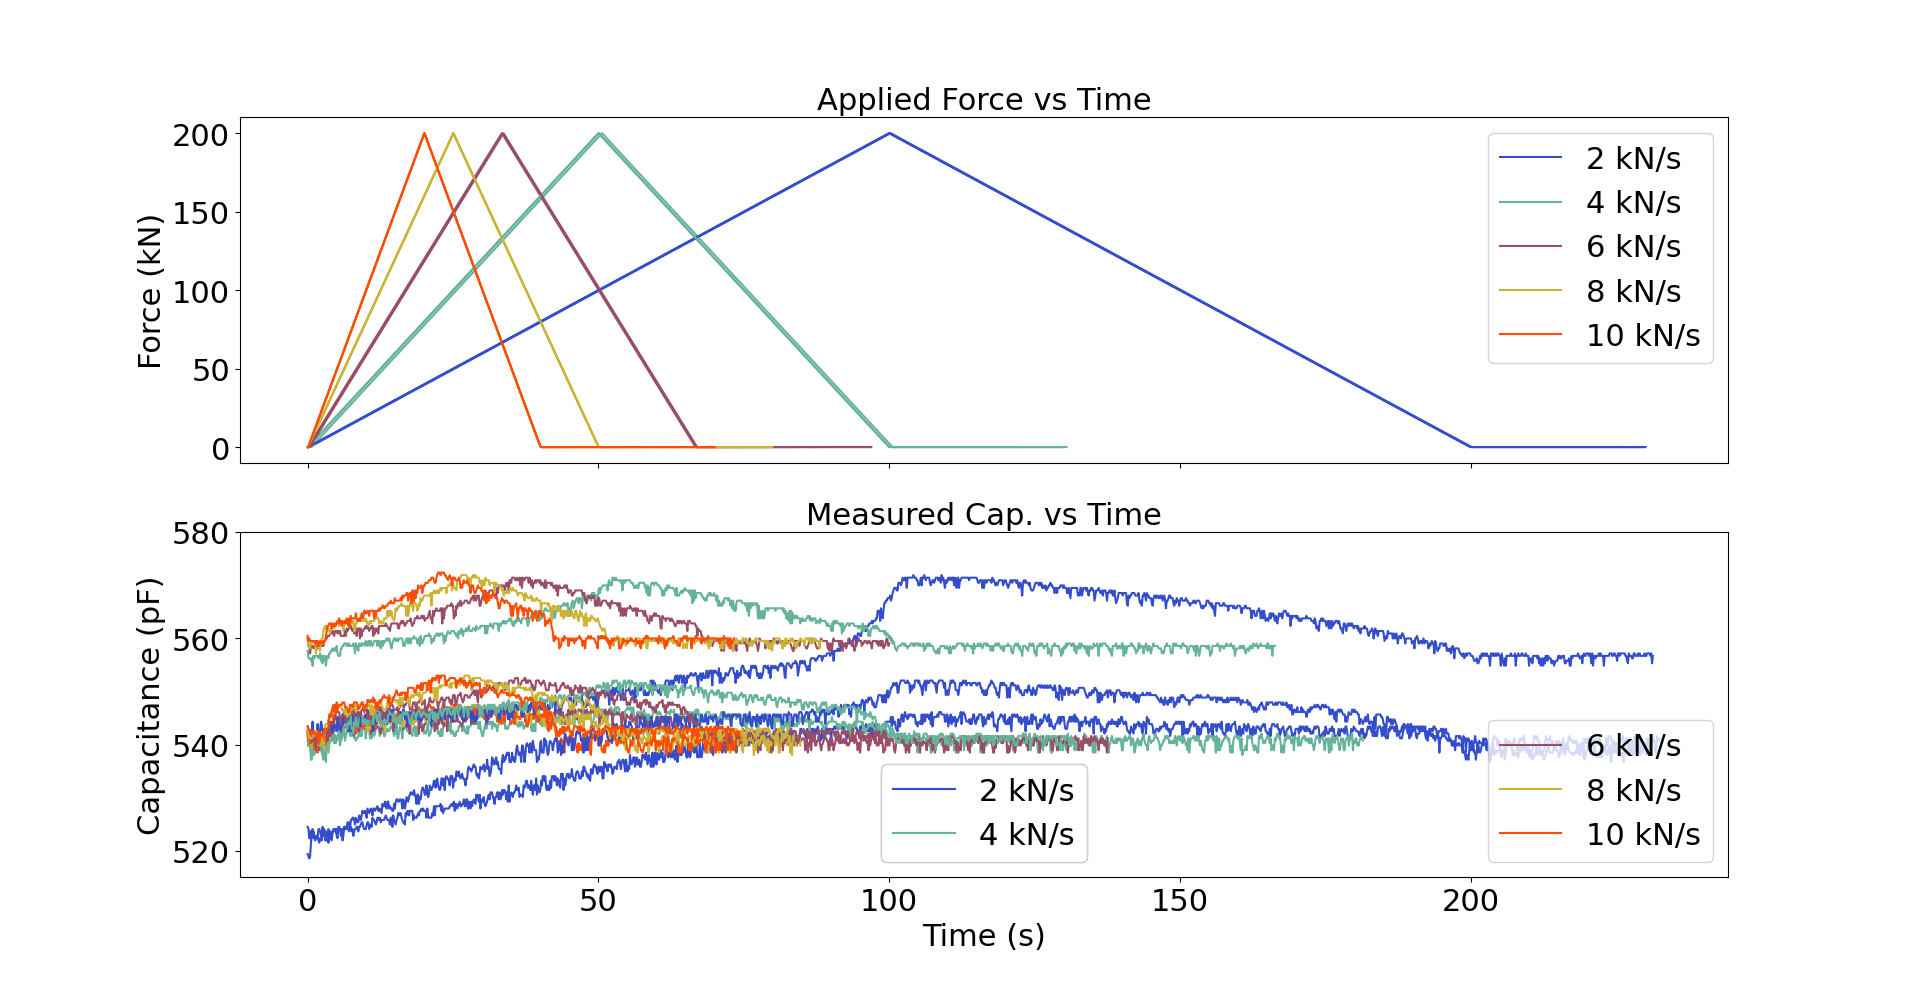
\includegraphics[width=5.5in]{figures/p1_media/Fig4.png}}
% sensor triangular tests
\caption{
The triangular load profiles and the resulting measurements from the sensor. 
The sensor response is not symmetric and therefore non-linear.
Lower load rates cause greater changes in displacement, which is consistent with previous studies for 
 thin film polyimide. 
}
\label{fig:triangleload}
\end{figure}

\begin{figure}[t!]
\centering
\centerline{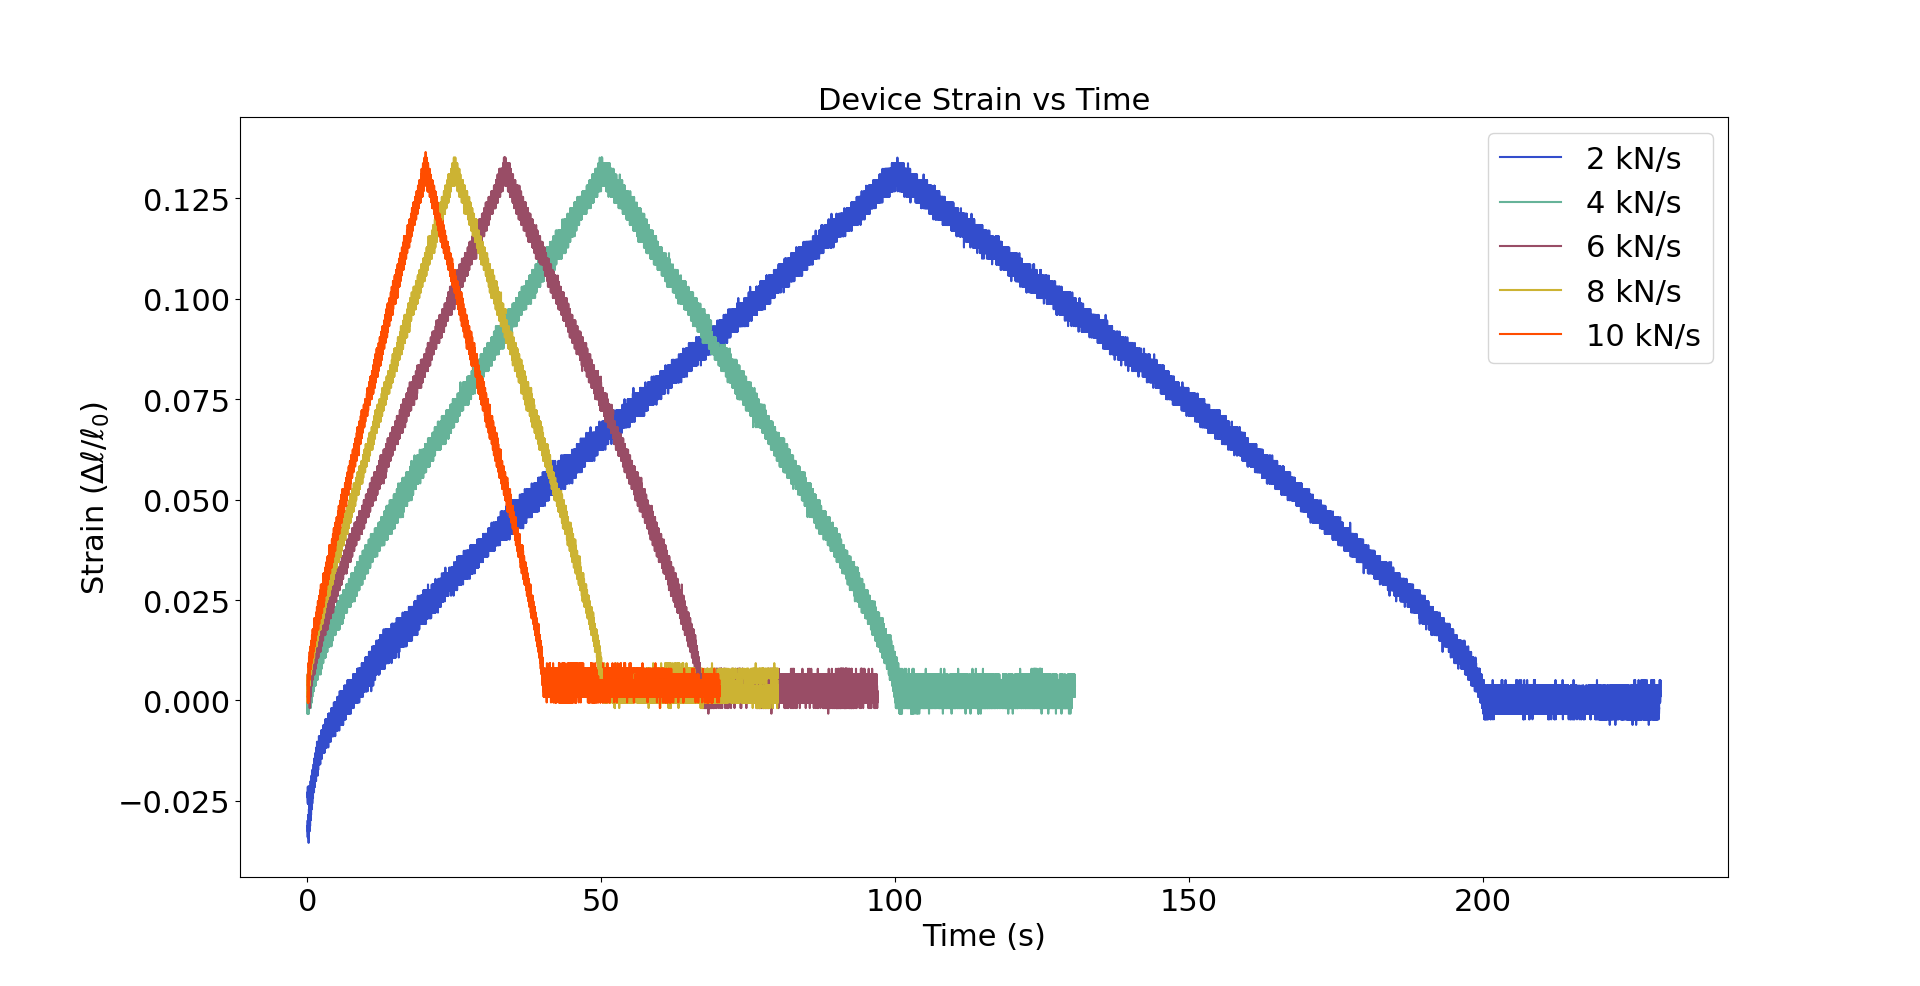
\includegraphics[width=5.5in]{figures/p1_media/Fig5.png}}
% sensor case deformation
\caption{
The case deformation during the load frame tests. The case deformation is symmetric for the 
 loading and unloading phases, it also has a consistent slope for force over displacement.
This means the case has approximately linear deformation for these load profiles.
}
\label{fig:casedeformation}
\end{figure}

\subsection{Rock Cutting Experiment}

To test the sensor for \textit{in-situ} force signature capture, rock cutting experiments
 were performed using the Linear Cutting Machine in the Earth Mechanics Institute at the 
 Colorado School of Mines.
A limestone sample cast in concrete was cut using a conical pick
 on the instrumented block. 
Time series measurements were made with the custom sensor as well as
 strain gauges integrated with the test equipment. 
The measurements were cut into small intervals and used with the classification 
 algorithms to build separate material and wear classifiers


To capture the capacitive measurements, a capacitance to digital converter made by
Texas Instruments is used: the FDC2114. This device interfaces with a generic 
microcontroller over I2C, a popular circuit to circuit interface. The software
used on the microcontroller is available on Github as well as the data-acquisition software
which is ran on the host computer to collect the measurements.
The software that performs the classification experiment described in the previous section is also available.
The microcontroller code is available here:  \url{https://github.com/Fworg64/DAQuery}.
The data-acquisition code is available here: \url{https://github.com/Fworg64/reDAQ}.
The machine learning and classification code is available here: 
\url{https://github.com/Fworg64/limestone_experiment}.


The Linear Cutting Machine, shown in \ref{fig:lcmaction},
 uses hydraulic actuators to drag the sample against the cutting tool.
A cutting speed of 10 inches per second was used, which is relatively slow 
 compared to the cutting speeds used in the field.
The integrated strain gauges measure forces at a rate of 537.6 samples per second. 
The custom load cell makes measurements at a rate of 400 samples per second.
The measurements from each sensor were recorded for use in the classification experiments.
For applications with greater cutting speed and more materials, 
 consider that rock fracture is largely static and machine vibration is dynamic.
The frequency domain features associated with tool wear should scale with cutting speed 
 and depend largely on the machine's natural modes, 
 while those associated with material breakdown occur at much higher frequencies.

\begin{figure}[t!]
\centering
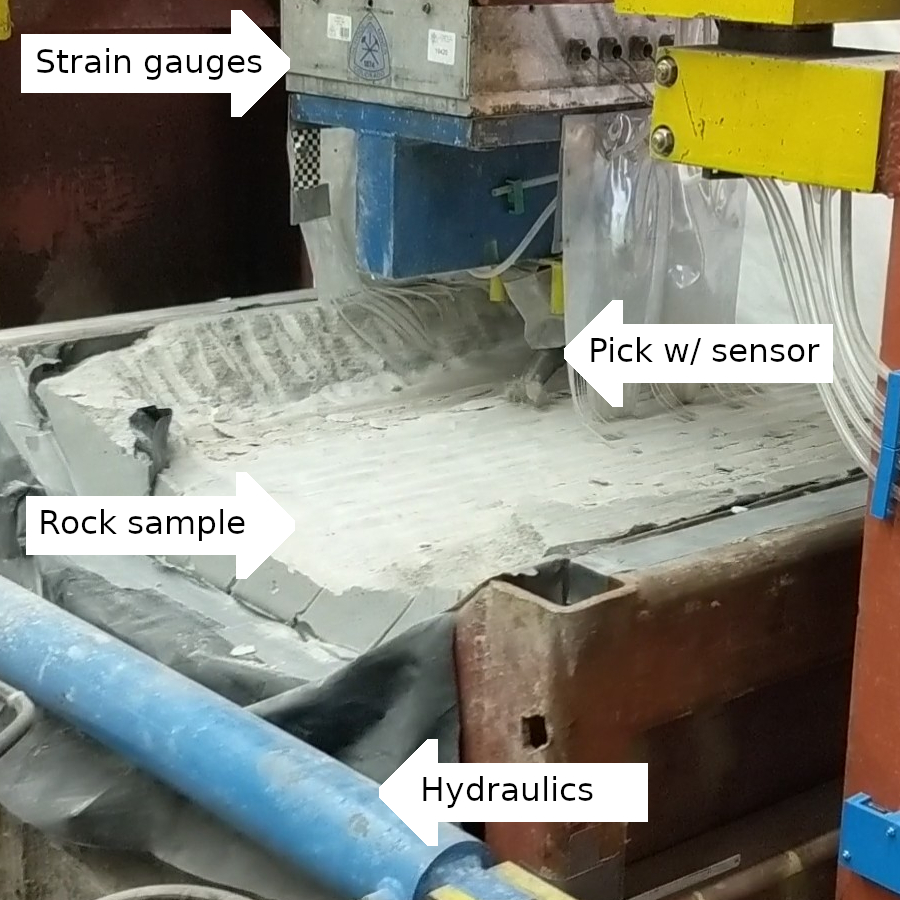
\includegraphics[width=3in]{figures/p1_media/Fig6.jpg}
%LCM figure
\caption{
The Linear Cutting Machine in action. Hydraulic actuators push the sample into the cutting tool
while the custom sensor and the embedded strain gauges record measurements. 
The tool is normally surrounded by the plastic curtain to aid in capturing dust for a 
 simultaneous study of the effect of tool wear on dust generation.
}
\label{fig:lcmaction}
\end{figure}

\subsection{Classification Results}

% Features after pre-processing
Using the method outlined in Section 2, the collected data is used to train and test
 the classification algorithm.
The capacitive sensor data gave results similar to the linear sensor in tool wear classification.
For material classification, the capacitive sensor generally performed better.
The distribution of feature vectors, before being processed with the support-vector machine kernel,
 are shown for both sensors by material in \ref{fig:matsigs} and by tool wear in \ref{fig:wearsigs}. 
From these distributions, it can be seen that the capacitive sensor is much more sensitive to the higher frequency 
 components of the interaction forces. 
This is likely a result of its closer proximity to the cutting interface.
Typical measurements from cutting experiments are shown in \ref{fig:cutforces}. 

% Distributions of scores by window size, significance
For each sensor and application, five window sizes were tested. 
This gives ten pairs for comparison among each group of five, 
 so we choose $p<0.01$ as statistically significant for differences in performance.
The distributions of F1 scores for the classifiers with different window sizes are shown in \ref{fig:windows}.
For tool wear classification, performance was similar for all window sizes for both sensors.
For material classification, the capacitive sensor gave measurements which could be more reliably classified.
The differences in performance across window sizes are significant for material classification with either sensor.

% Results 
Classification scores broken down by technique for the 0.2 second window size are shown in \ref{fig:methods}.
Trends in relative method performance were the same across window sizes.
It was found that normalization after transformation, and not before, gave the best performance for 
 the Fourier based methods.
Also, the normalized time-series data with the SVM gave the best performance for 
 tool wear classification in both the strain gauge and capacitive sensor cases.
For material classification with the strain gauges, most methods gave similar performance.
Normalization improved classification performance in nearly all categories.

Overall, tool wear in our data was classified with greater accuracy than material type. 
For tool wear, the normalized time domain data gave better classification results than
 the frequency data.
For material type, only the capacitive sensor gave results that would be useful. 
The strain gauge data was classified with about 50\% accuracy by the classifier.
With the capacitive sensor classification of material type, 
performance using the frequency based data gave slightly better accuracy than the time
domain data.

When using only 25\% of the data for training, the classifier was still able to perform
reliably using the capacitive sensor data. 
This shows that performance was not very dependent on the test and train ratio.
F1 scores with standard deviations are given for the best setup for each application 
 at different test and train ratios in Table~\ref{tab:fourscores}.
The scores do not change by a large magnitude, which indicates that 
 the classifier is general and should perform well for larger data sets.

Individual confusion matrices are given for the 25:75 test and train ratio for 
 material classification in Table~\ref{tab:mat_conf} 
 and for tool wear classification in Table~\ref{tab:wear_conf}.
For these confusion matrices, rows represent the true class for the samples and columns represent the 
 predicted class. Diagonal entries represent correct classifications, 
 and each column is normalized to the number of predictions made of that class.
The strain gauge material classifier has poor precision for concrete samples, 
 as many of its concrete predictions are actually limestone samples. 
The F1 score is sensitive to this, and it is reflected in the much lower score.
The accuracy of the strain gauge material classifier is around 80\%, which 
 is still useful. 
The accuracy of the capacitive sensor material classifier is higher, above 95\%.
This highlights the importance of using multiple metrics to 
 accurately assess classifier performance.

\begin{figure}[t!]
\centering
\centerline{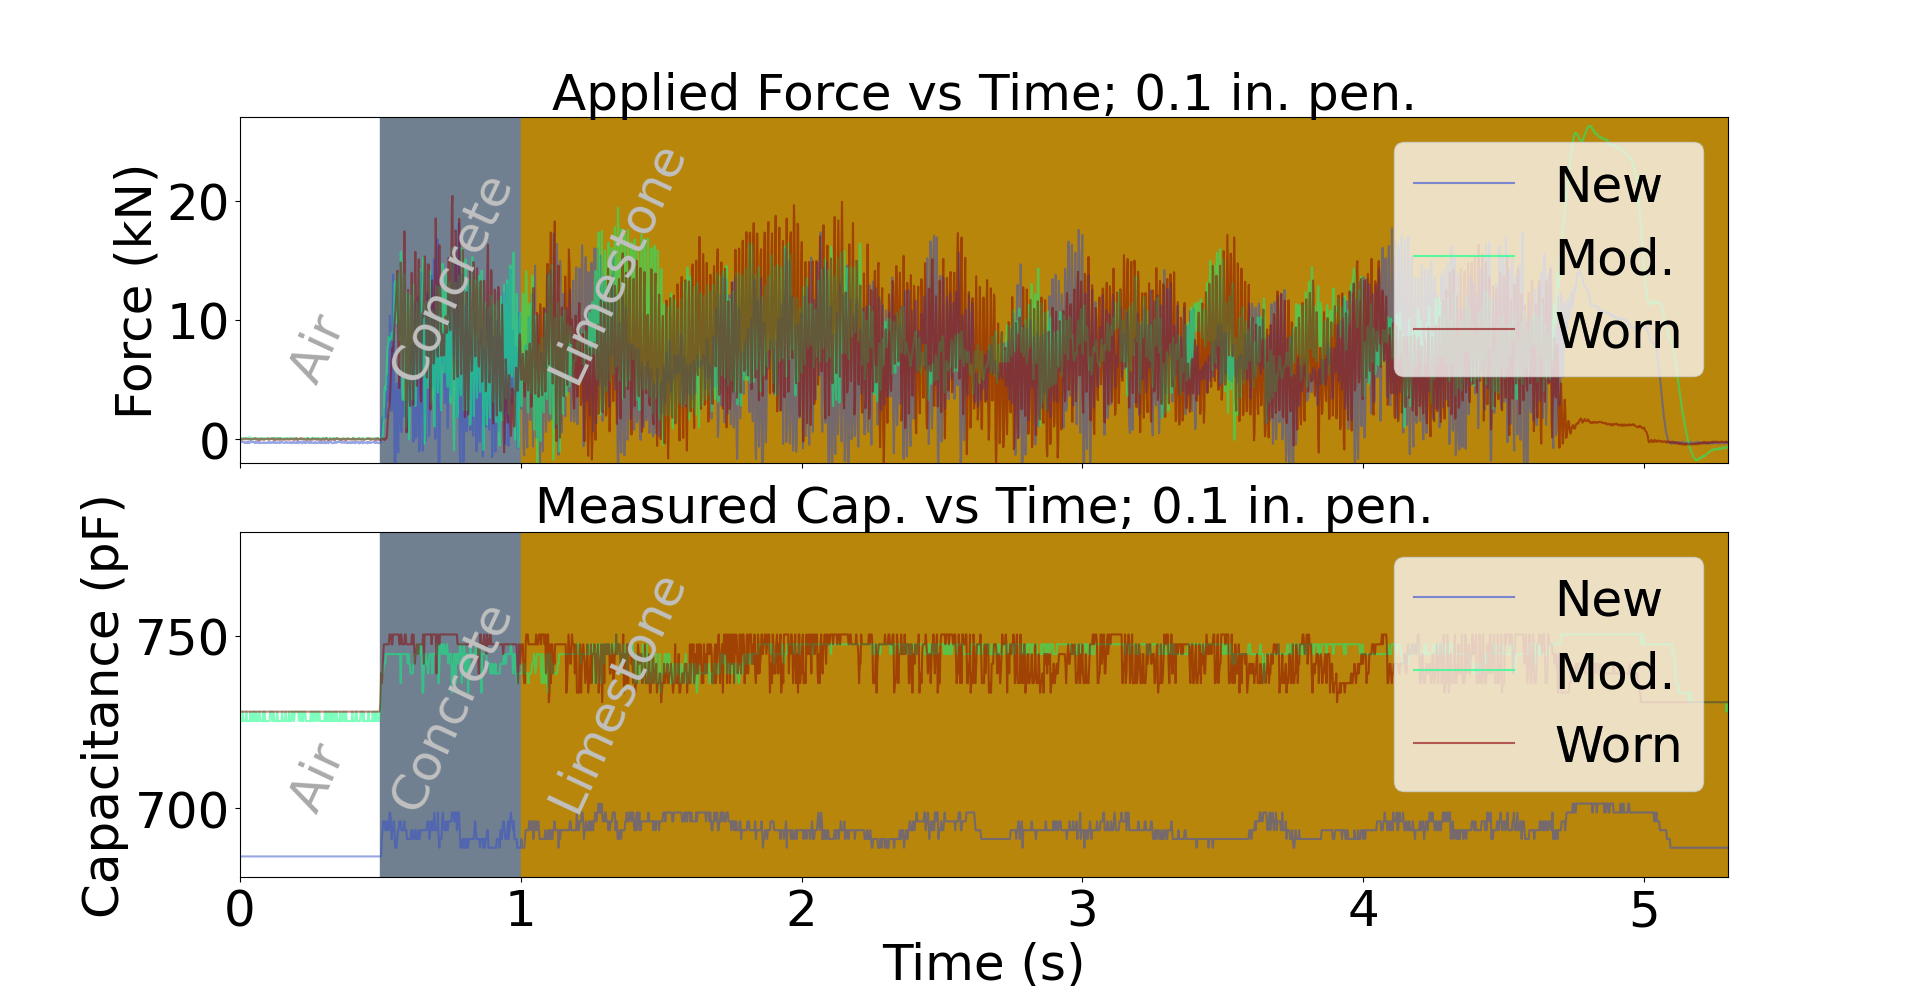
\includegraphics[width=5.5in]{figures/p1_media/Fig7.png}}
%cutting measurements
\caption{
Measurements for typical rock cuts with different tool wear levels. The measurements from the 
linear sensors are shown in the top graph while the measurements from the custom sensor are shown below.
}
\label{fig:cutforces}
\end{figure}

\begin{figure}[t!]
\centering
\centerline{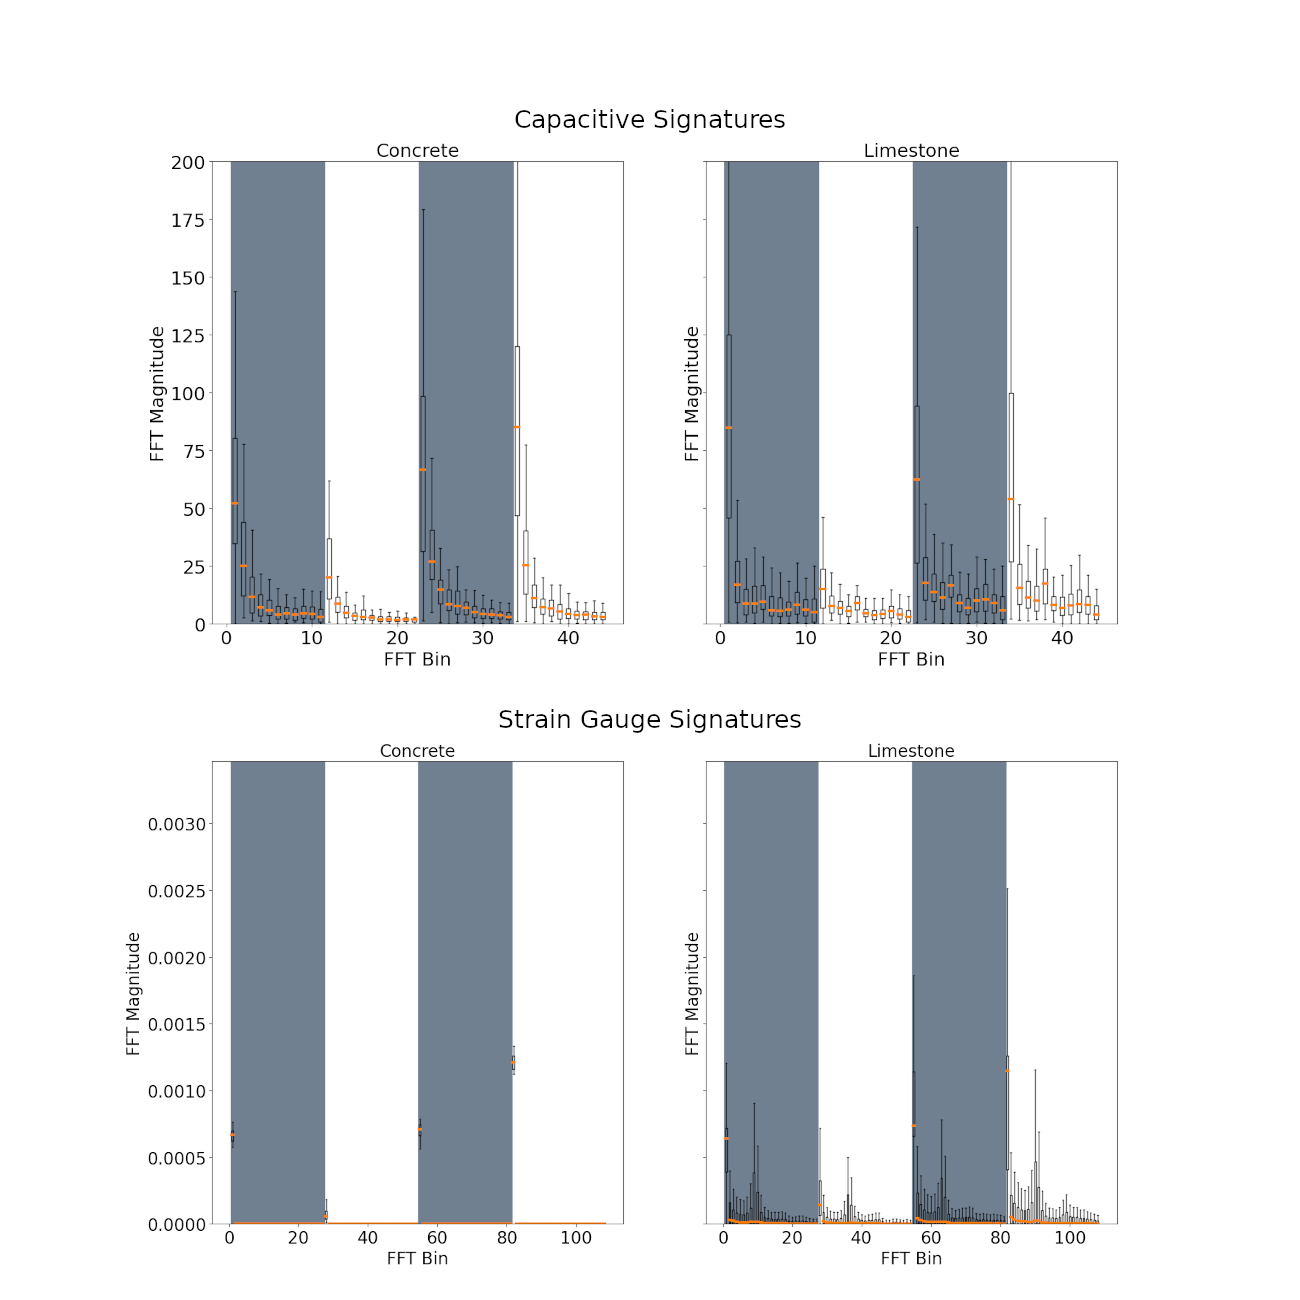
\includegraphics[width=5.5in]{figures/p1_media/Fig8.png}}
%material sigs
\caption{
The frequency signature distributions collected from the custom sensor organized by material.
The concrete material shows exponential decay after each primary mode, while the limestone 
 has a more varied response. These differences can be used for classification of the signals by material.
}
\label{fig:matsigs}
\end{figure}

\begin{figure}[t!]
\centering
\centerline{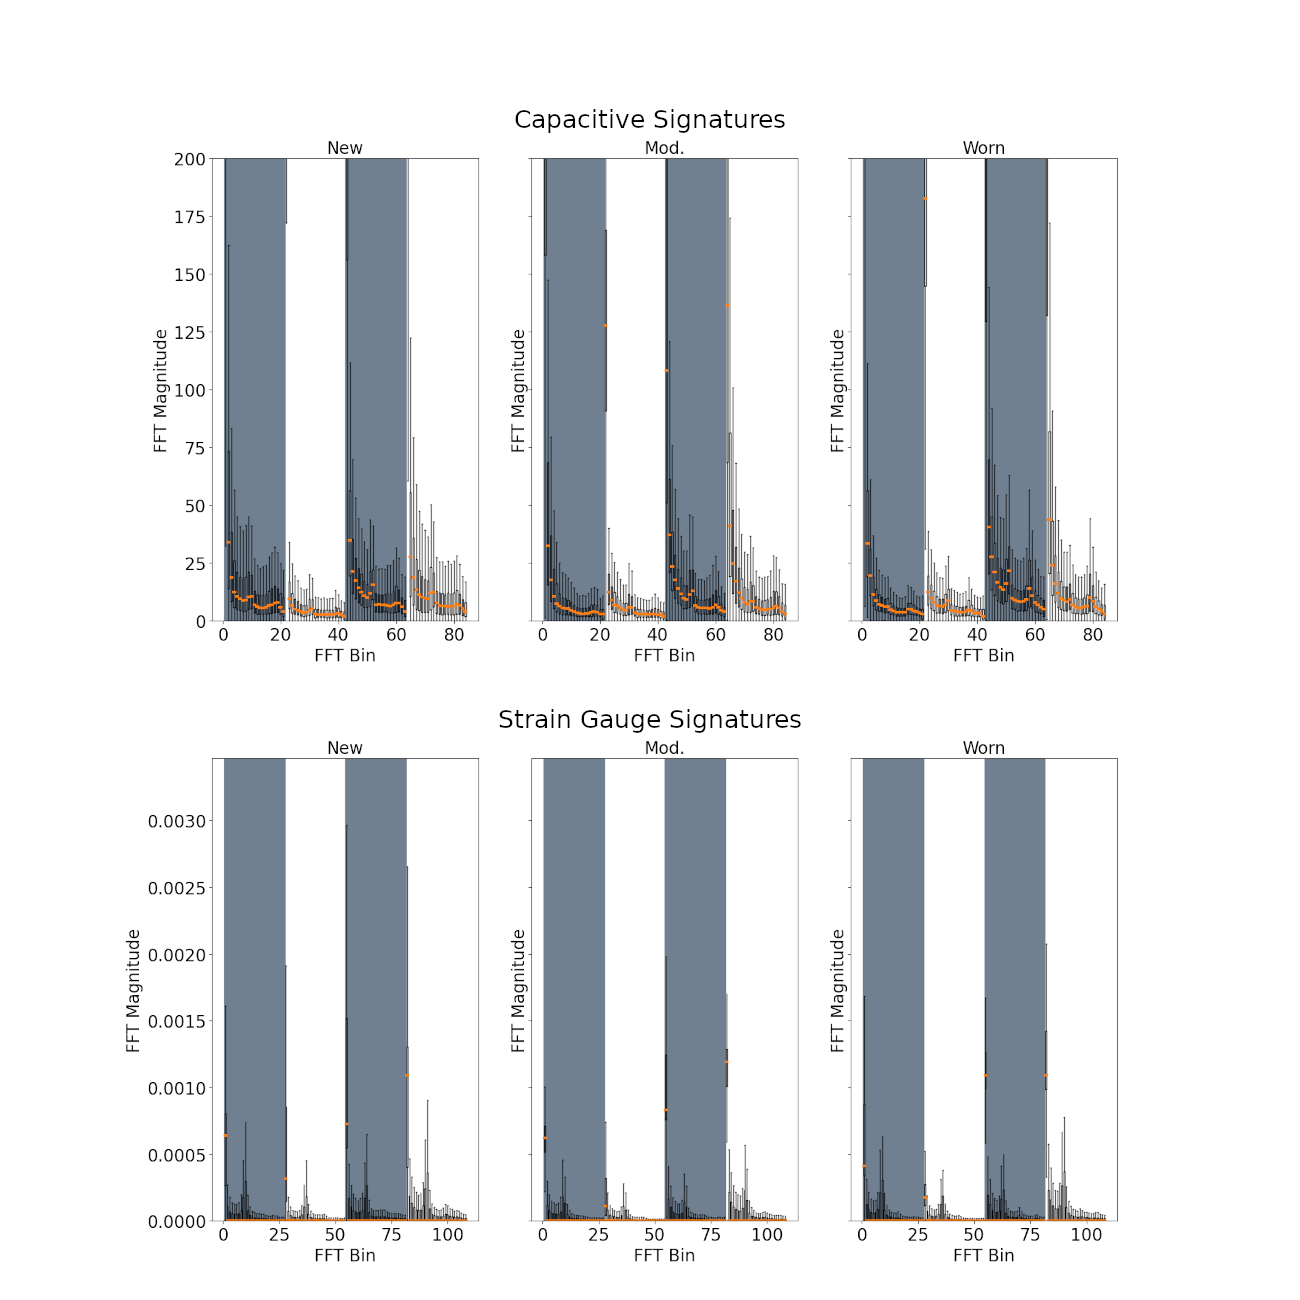
\includegraphics[width=5.5in]{figures/p1_media/Fig9.png}}
%wear sigs
\caption{
The frequency signature distributions collected from the custom sensor organized by tool wear.
The New tool has a distinct response compared to the Moderate and Worn tools, and the 
 energy in the higher modes generally increases with wear.
These differences can be used for classification of the signals by tool wear.
}
\label{fig:wearsigs}
\end{figure}

\begin{figure}[t!]
\centering
\centerline{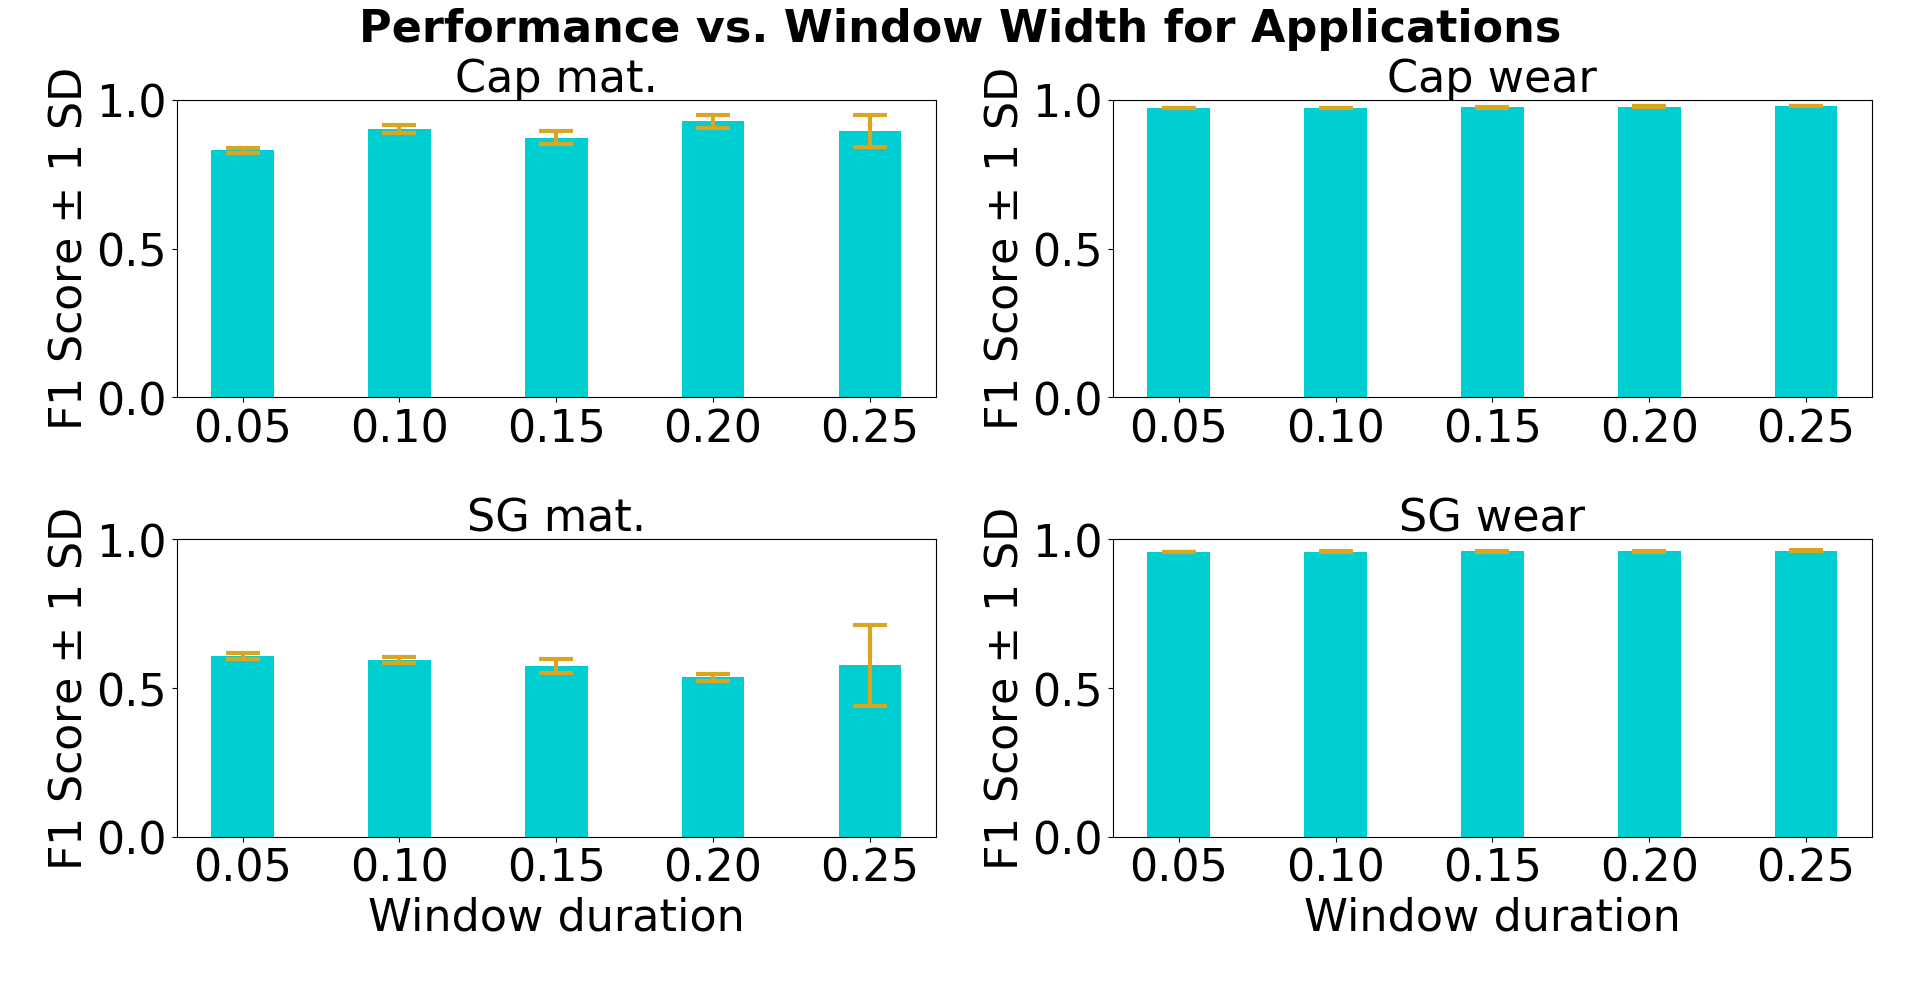
\includegraphics[width=5.5in]{figures/p1_media/Fig10.png}}
%Windows
\caption{
Bar chart with error bars for F1 score distributions by window size. For tool wear, both
 sensors were able to provide sufficient data for very accurate classification.
For material classification, the capacitive sensor generally performed better than the
 strain gauge sensor. Some of the differences in performance are significant within the 
 application and sensor combinations, but in general performance was similar across window sizes.
}
\label{fig:windows}
\end{figure}

\begin{figure}[t!]
\centering
\centerline{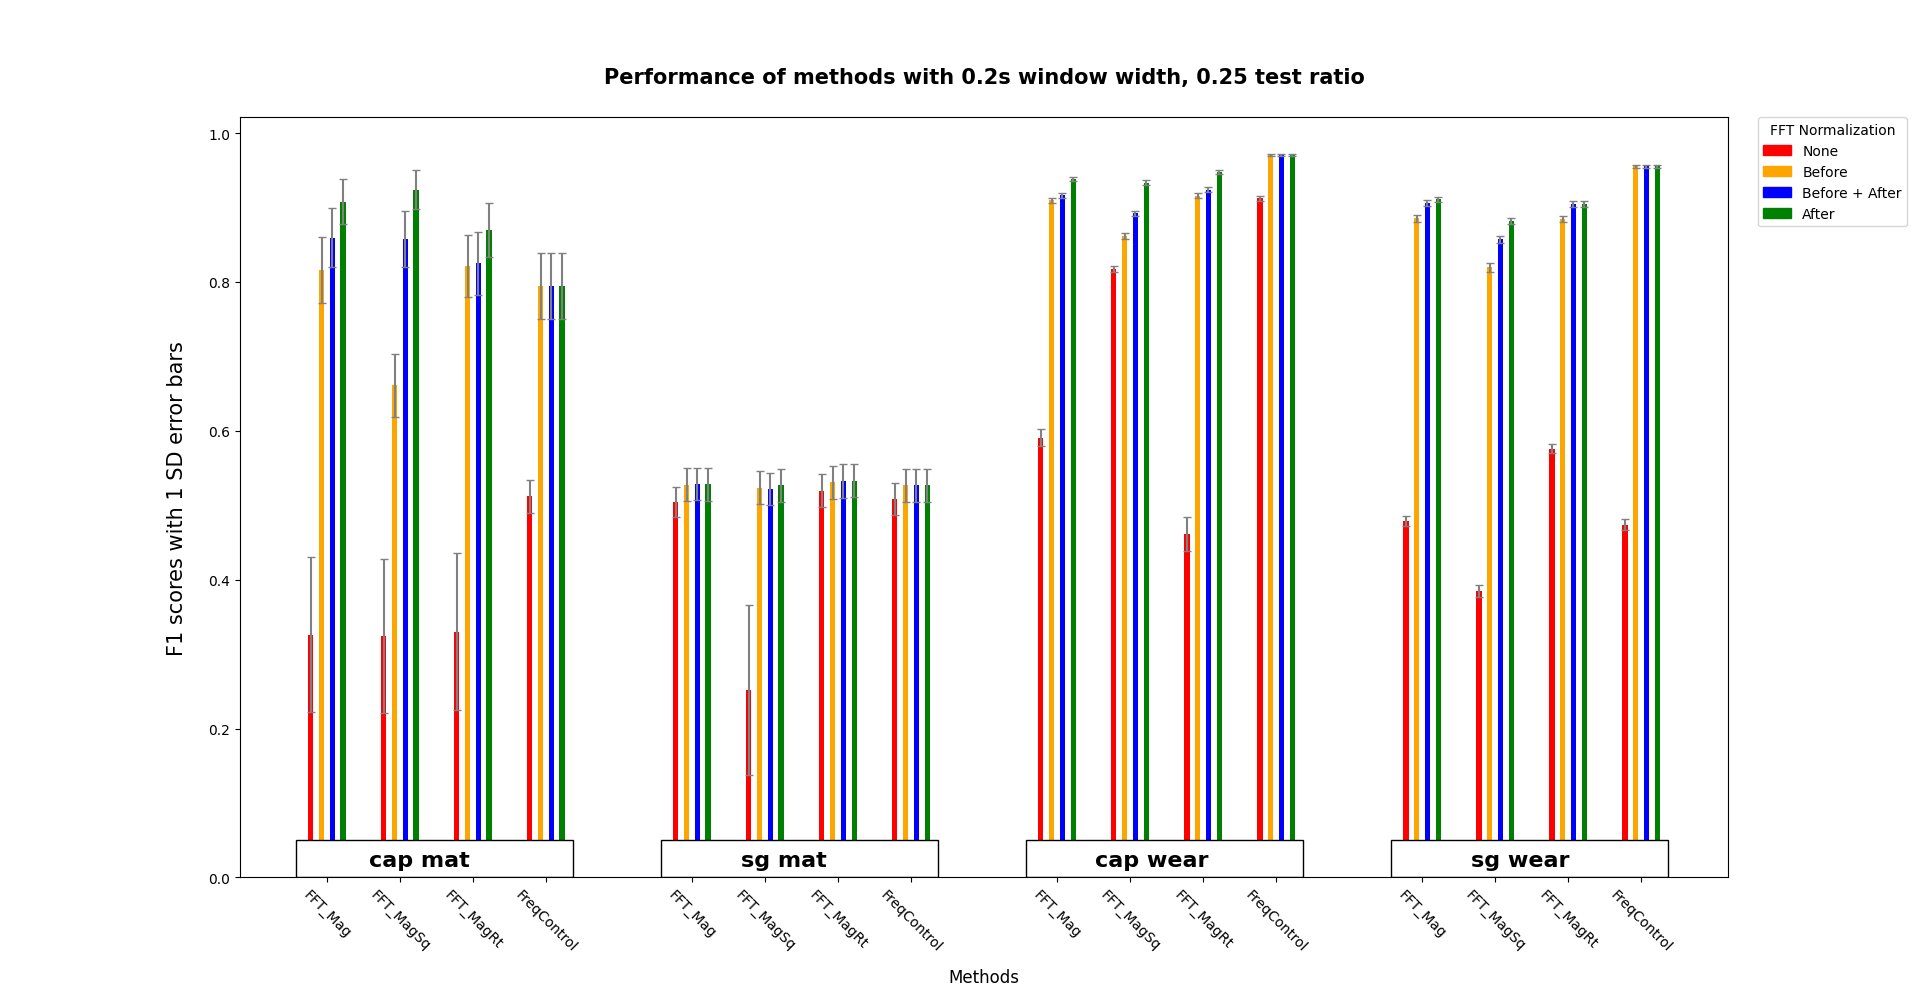
\includegraphics[width=5.5in]{figures/p1_media/Fig11.png}}
%Methods
\caption{
Performance of different preprocessing methods for each application. In general, normalization
 after transformation proved most effective for the frequency based techniques. 
 Using the normalized time domain data was most effective for tool wear classification.
}
\label{fig:methods}
\end{figure}

% Please add the following required packages to your document preamble:
% \usepackage{multirow}
\begin{table}[]
\caption{Scoring metric and test/train ratios for each application}
\begin{tabular}{lll|lll}
\multicolumn{3}{l|}{F1 Scores (mean $\pm$ std. dev., 100 trials)}                                                        & \multicolumn{3}{l}{Test and Train Ratio} \\ \hline
Application                                     & Sensor                    & Best Config.                
   & 25:75      & 50:50      & 75:25      \\ \hline
\multicolumn{1}{l|}{\multirow{2}{*}{Tool Wear}} & \multicolumn{1}{l|}{Cap.} & Time Domain 
   & $0.971 \pm  0.003$   & $0.965 \pm 0.003$ & $0.950 \pm 0.004$  \\ \cline{2-6} 
\multicolumn{1}{l|}{}                           & \multicolumn{1}{l|}{SG}   & Time Domain 
   & $0.955 \pm 0.005$    & $0.947 \pm 0.004$ & $0.934 \pm 0.004$  \\ \hline
\multicolumn{1}{l|}{\multirow{2}{*}{Material}}  & \multicolumn{1}{l|}{Cap.} & FFTMagSq 
   & $0.924 \pm 0.053$    & $0.902 \pm 0.044$ & $0.831 \pm 0.085$  \\ \cline{2-6} 
\multicolumn{1}{l|}{}                           & \multicolumn{1}{l|}{SG}   & FFTMagRt 
   & $0.533 \pm 0.045$    & $0.536 \pm 0.026$ & $0.534 \pm 0.016$  
\end{tabular}
\label{tab:fourscores}
\end{table}

\begin{table}[h]
\centering
\caption{Confusion Matrix for Material Classifier; Normalized by prediction \newline
         New Picks, 0.3 in Penetration, 0.2s Window, 50:50 test and train, PSD w/ post norm.}
\begin{tabular}{l|ll|ll}
\% Pred.   & \multicolumn{2}{l|}{Strain Gauge Prediction}                & \multicolumn{2}{l}{Cap. Prediction}                          \\ \hline
True Class & \multicolumn{1}{l|}{Concrete} & \multicolumn{1}{l|}{Limestone} & \multicolumn{1}{l|}{Concrete} & \multicolumn{1}{l|}{Limestone} \\ \hline
Concrete   & 0.117& 0.000                     &  0.923                    & 0.013\\
Limestone  & 0.883& 1.000                     &  0.077                    & 0.987
\end{tabular}
\label{tab:mat_conf}
\end{table}

\begin{table}[h]
\centering
\caption{Confusion Matrix for Tool Wear Classifier; Normalized by prediction \newline
         All Materials, All Penetrations, 0.2s Window, 50:50 test and train, Normalized Time Domain Data}
\begin{tabular}{l|lll|lll}
\% Pred.   & \multicolumn{3}{l|}{Strain Gauge Prediction}                & \multicolumn{3}{l}{Cap. Prediction}                          \\ \hline
True Class & \multicolumn{1}{l|}{New} & \multicolumn{1}{l|}{Mod.} & Worn & \multicolumn{1}{l|}{New.} & \multicolumn{1}{l|}{Mod.} & Worn \\ \hline
New         & 0.983   & 0.105  & 0.000      & 1.000     & 0.000     & 0.000 \\
Mod.        & 0.016   & 0.893  & 0.015      & 0.000     & 0.980     & 0.082 \\
Worn        & 0.001   & 0.002  & 0.985      & 0.000     & 0.020     & 0.918
\end{tabular}
\label{tab:wear_conf}
\end{table}

\subsection{Discussion}

Our sensor, as used in our experiment, shows promise as a method to objectively assess material type and tool wear.
Under laboratory conditions, the sensor and classification scheme was able to detect differences in 
mode excitation caused by different materials and tool wears. For our experiment, the materials chosen were
limestone and concrete. These materials are both much stronger than coal, but our experiment shows that they
excite distinct modes in our cutting equipment. For tool wear, it is known that more worn tools can
require several times the force to cut when compared to a new tool. The modes that are excited in the
machine also change based on the changing tool geometry. For the target application of coal mining,
coal is known to be much weaker than the material in which it is embedded, e.g. limestone. 
So, if our sensor is able to differentiate between concrete and limestone,
 it is postulated that it could differentiate between limestone and coal, which is much softer.

Using the Support-Vector Machine, the hyperplane between the measured datasets is found. 
This means that for a given input of discrete frequency or time samples, each value is 
 multiplied by a coefficient and then combined to a single value, similar to a digital filter. 
The Support-Vector Machine has few hyperparameters, and the chosen measurements 
 are shown to contain modal shifts that correspond with the categories of interest. 
The fundamental change in signal occurs as a mode distribution shift.
This is readily detected by the Support-Vector machine.

To adapt our sensor to the target application, 
the target machine would need to be characterized in terms of dynamic modes.
The sampling rate of the sensor system will need to be sufficiently higher than
the primary modes of the target tooling, otherwise the measurements could be subject to aliasing.
So long as the sampling rate at least satisfies the Nyquist criterion for the tool primary modes,
aliasing should be minimized due to the high frequency attenuation caused by massive mechanical systems.
Further, the viscous nature of the polyimide sensor provides even more damping, reducing the possibility
for aliasing at the physical level.

Additional sensor designs such as an air-gap capacitive displacement sensor should also be investigated,
 as they could likely achieve more linear measurements at the cost of sensitivity.
Development of a suitable power source and communication system must still be considered for this
application.
Other technologies such as acoustic sensors also show promise for material and wear classification,
 as they have been used with success in other domains and acoustic information is one of the primary 
 feedback mechanisms currently employed by operators. A load cell based technology would likely
be less susceptible to outside interference by unrelated signal when compared to an acoustic sensor,
as it is closer to the mining interface and collects signal from a more narrow bandwidth.

\subsection{Conclusion}

A sensor suitable for \textit{in-situ} sensing of vibration signatures for material and wear classification
 was developed and tested for underground mining using conical picks. 
The classification accuracy achieved in the laboratory tests indicates that this is a promising 
 technology for this application.
The capacitive sensing design is low cost and low power due to its flexible circuit design.
This technology could assist operators in material and wear classification by providing an objective
 measurement without requiring the operators to enter known hazardous regions near the machine and mining interface.

The capacitive load cell, to the authors knowledge, has not been used publicly for conical picks in 
rock cutting applications. This is a relatively new sensor technology that has been enabled by the 
steady advancement of capacitive sensor research over the last few decades.
Existing solutions for hazard monitoring in underground coal mining primarily identify problems
after they begin. 
Existing research in improving operator performance
and safety has included acoustic classification systems and algorithms, strain-gauge based solutions, 
and piezo-electric sensors.
By shifting the paradigm to predictive maintenance and more responsive control,
 operators are enabled to be safer and more efficient. 

\subsection{Disclosures}

\subsubsection{Conflicts of interests}
On behalf of all authors, the corresponding author states that there is no conflict of interest. 
This work was funded by NIOSH Contract 75D30119C05413, ``IMPROVING HEALTH AND SAFETY OF MINING OPERATIONS
THROUGH DEVELOPMENT OF THE SMART BIT CONCEPT FOR AUTOMATION OF MECHANICAL ROCK EXCAVATION
 UNITS AND DUST MITIGATION''.

%\subsection{References}
%\bibliography{supporting-files/sources_flexpcb}% common bib file


% \addtocontents{toc}{\vspace{31\baselineskip}} % This line moved the Chapter 5 TOC entry to the next page to be with it's subheadings.

\chapter{Tool Wear Classification for Conical Picks
using Acoustic Fourier Spectra Magnitude \label{chap:P2}}

\begin{center}
This article has been published open access and is part of the public domain.
The copyright remains property of the author.
\end{center}

\subsection{Abstract}

Underground coal mine workers who operate continuous mining machines 
rely on many cues to determine tool wear. 
This skill is difficult to train and proximity to the
mining interface is a hazard to the machine operators. 
To create safer conditions for machine operators, we propose an acoustic classification method for determining tool wear.
To demonstrate this technique, we cut a concrete sample with conical picks of different wear levels
 using a linear cutting machine and record the acoustic data for classification experiments.
We highlight the differences in acoustic frequency spectra and
 demonstrate classification of short segments of the recorded acoustic data, less than 100 milliseconds in duration,
using three popular classification techniques: the K-nearest neighbors classifier, 
 the support-vector machine classifier, and the multi-layer perceptron classifier. 
We compare the performance of the techniques and also examine the effects of segment size and downsampling.
Of our tested methods, the support-vector machine gives good performance with little complexity.
This technology could aid operators in performing their roles from a safer distance, 
alerting them to worn tool conditions in real time.


\subsection{Introduction}\label{sec1}

Underground mining safety has not improved over the last decade, with the rate of fatalities
per 100,000 Full Time Equivalent (FTE) workers remaining around 21.4 from 2011 to 2020 \cite{nioshdata}. 
In the literature review conducted by Sari et. al., it is noted that younger, less experienced
miners are at greater risk of suffering a disabling injury \cite{Sari2004}.
On the other hand, for older and more experienced miners, 
the high levels and long duration of exposure to the hazards inevitably leads to problems
like hearing loss \cite{Erol2022}, or other diseases such as black lung, 
a serious lung disease caused by exposure to coal dust, which can be fatal \cite{Colinent2020}.

Some examples of dangers in the underground mine environment include: 
tunnel collapse, explosive gasses \cite{Juganda2022},
high temperatures \cite{cinar2020}, exposure to diesel particulate \cite{Bugarski2022},
and the crush hazards caused by machines used for the operation \cite{Swanson2019}.
Machine operators in underground coal mines are particularly at risk,
as they must remain near the cutting interface to pick up cues from machine and the environment
to monitor cutting conditions \cite{Bartels2009}.
Workplace accidents caused by these hazards is problematic and they lead to 
loss of productivity, worker injury, and loss of life \cite{sensogut2021}.
The National Institute for Occupational Safety and Health (NIOSH), 
recommends removing workers from hazardous locations as the best form
of risk reduction in general \cite{niosh_2015}.

Aiding operators with improved sensors for tool wear detection can help them 
perform their role from a greater distance to the cutting interface and 
reduce their risk from dust exposure as well as the from the immediate dangers at the cutting interface.
Experienced operators are an invaluable resource, 
 as they hold the experience gained after years of dealing with hazardous conditions \cite{Bartels2009}.
Operators are known to rely on many cues, including visual, acoustic, and vibrational.
This suggests a sensor can measure these cues.

Acoustic sensors can operate with a quick, less than one second, response time and detect changes in 
material type and tool wear in many domains \cite{Zakeri2017, Zhong2013, Rad2014, Zakeri2015}.
When comparing acoustic, visual, and vibrational cues for tool wear,
acoustic detection of tool wear has the advantage over visual detection in that it
does not require a clear line of sight to the cutting interface, 
which is often in a hazardous location near the machine \cite{Bartels2009}.
Alternatively, vibrational cues require direct contact with the cutting process, 
which requires a more robust sensor design compared to an acoustic sensor which is placed further away.
We choose to investigate using acoustic data for objective tool wear classification from a distance.

Any technology that is employed in this domain must be well suited for the task it is
designed to perform, or else its adoption is unlikely \cite{Swanson2019}.
By providing objective, real time data to human operators, 
our proposed technology can help operators make objective decisions 
regarding shutting down operations for cost-saving maintenance or continuing work.
Automating tool wear detection can also allow machine operators to focus on other aspects of machine operation, 
increasing their productivity.
Automation also enables collection of data that could be analyzed for trends in tool wear during operation.

The rest of this article is outlined as follows. 
In the Background subsection, the application background
 and previous work used to guide this study are discussed.
The Methods subsection follows, and it gives detailed description of the 
 experimental equipment, classification methods, and metrics for comparing classification performance.
After that, the Results subsection lists the notable results.
Then, a Discussion subsection is given, which states the merits of the tested methods 
 and provides recommendations for implementation.
Finally, a Conclusions subsection summarizes the work and its relevance considering the target application.

\subsection{Background}\label{sec1a}

In the black lung study by Colinent, the author notes that much effort has been given to dust mitigation.
Strategies include: minimizing dust generation, preventing dust from circulating, removing
dust from circulation, diluting dust concentration, use of barriers and ventilation direction
to reduce worker exposure, and maintenance of these systems \cite{Colinent2020}. 
The idea of removing workers from hazardous zones is supported 
 by the general advice given by NIOSH in their hierarchy of controls \cite{niosh_2015}.
In order to remove workers from the hazardous zones, they must be enabled to perform their roles from 
more remote locations. 

Considering that experienced human operators are able to detect tool wear using acoustic cues
suggests that enough relevant information can be captured within the typical human hearing range.
A study on occupational hearing loss in underground mines reported that the type of hearing loss experienced 
by underground coal miners indicates a noise frequency below 6 kHz and a noise intensity 
around 90 dBA \cite{Erol2022}. 
We aim to capture these low frequency and high intensity acoustic emissions for classification.

As early as the 1990's, methods which consider the total volume of the acoustic emissions,
the count of peaks and valleys in the signal, and the changes in signal spectra 
have been researched \cite{Tan1992,Kakade1995}.
Proper preprocessing is important. 
In underground mining, the rock cutting system can lose mass as tools are worn,
resulting in a non-stationary dynamic system.
Fast Fourier transform based preprocessing of a small window of signal
 and subsequent classification with a support-vector machine has shown 
 to be an effective method for robust classification of non-stationary dynamic systems \cite{xu2016fftsvm}.

Other preprocessing techniques for similar problems include wavelet and Empirical Mode Decomposition.
Wavelet preprocessing combined with machine learning
has been used with success in recent years 
 \cite{he2013vibration, sadegh2016classification, skariah2021health}.
Empirical Mode Decomposition has demonstrated vibration classification for tool wear
 in other domains \cite{Xu2009, Nie2011, Zhan2014}.
We choose fast Fourier spectra magnitude based preprocessing and normalization for its time-invariant properties,
small number of hyperparameters, and known effectiveness across domains \cite{Xu2016, Harlianto2022}.

Both wavelets and Empirical Mode Decomposition are time-variant.
The wavelet transform is known to be very sensitive to small time translations \cite{Yen1999}.
With wavelets, this can be mitigated by measuring the average energy for 
a continuum of offsets and using those values 
as the feature vector for classification \cite{Baccar2015}.
Similar processing would be needed for Empirical Mode Decomposition. 
Another option is to register the signal in the time domain to an event, such as contact with the material.

We motivate our choice of preprocessing methods with the idea that different tool wear levels in a conical pick
will produce different acoustic emissions with different Fourier frequency spectra magnitude for a given material. 
We verify this by analyzing objective differences in statistical distributions 
of the frequency spectra magnitudes for the tested categories.
To leverage these differences, we employ and compare different classification techniques.
These methods and how they are compared are described in the next subsection.

\subsection{Materials and Methods}\label{sec2}

A homogeneous concrete sample is cut using the Linear Cutting Machine
at the Earth Mechanics Institute at the Colorado School of Mines, shown in \ref{fig:setup},
and capable of testing with many cutting tools \cite{THYAGARAJAN2024105675}. 
Acoustic data is recorded at a sample rate of 44.1 kHz using a digital camcorder,
and then the data is categorized by tool wear condition.
The different tool wear levels are shown in \ref{fig:levels}.
The tool tips have been artificially worn with a lathe to a spherical shape to approximate even wear.
They vary in diameter and have been chosen to represent a new, a moderately used, and a worn tool.

\begin{figure}[t!]
\centering
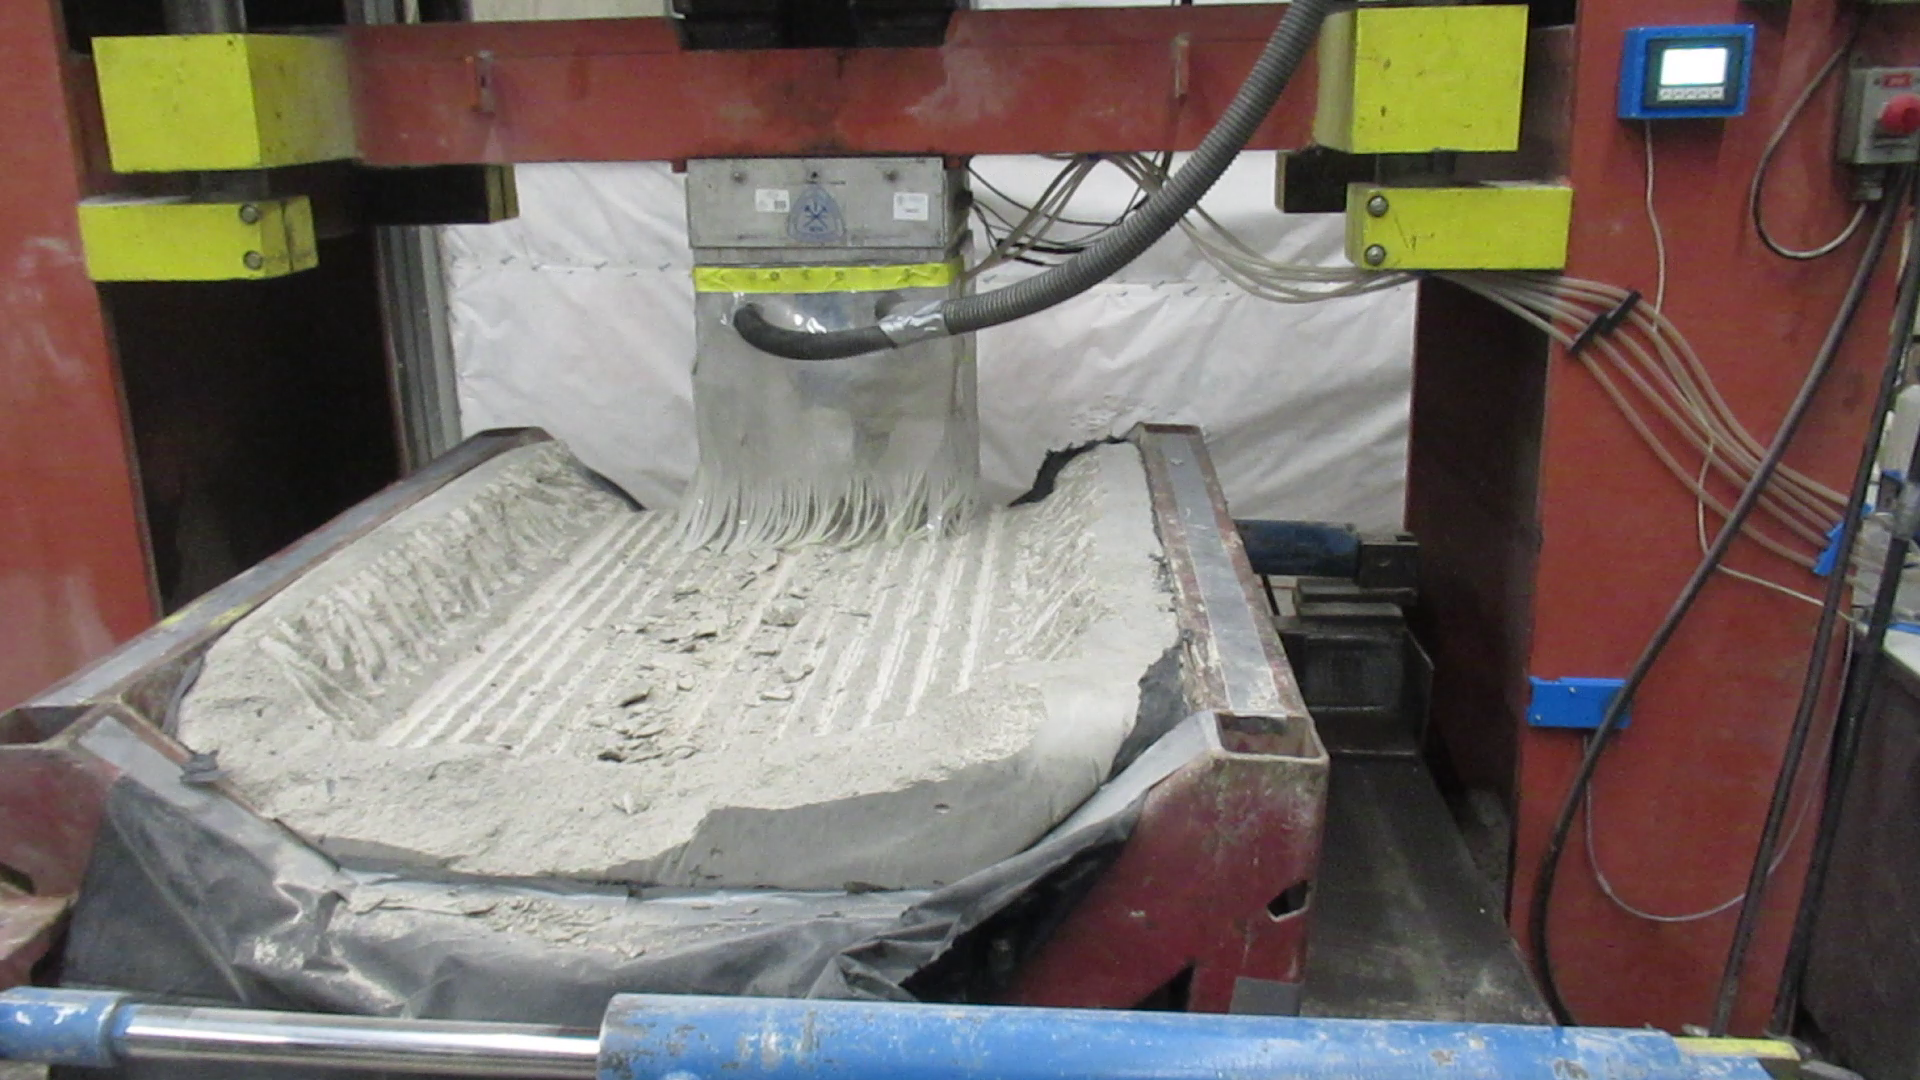
\includegraphics[width=5.5in]{p2_media/figures/raw/setup.png}
\caption{The Linear Cutting Machine at the Earth Mechanics Institute of Colorado School of Mines.
Hydraulic actuators move the rock box for positioning and cutting. The rock sample in this experiment
is a solid block of concrete. This is a homogeneous material that will isolate the changes in tool wear.
Additional equipment consisting of a dust shroud and vacuum sample collection system was used for a
 simultaneous study on dust generation, but not for this study.
Forces are recorded using integrated load cells in the coupling between the tool and the frame.
The acoustic signals for this experiment were recorded from the camcorder used to take this image.
}
\label{fig:setup}
\end{figure}

\begin{figure}[t!]
\centering
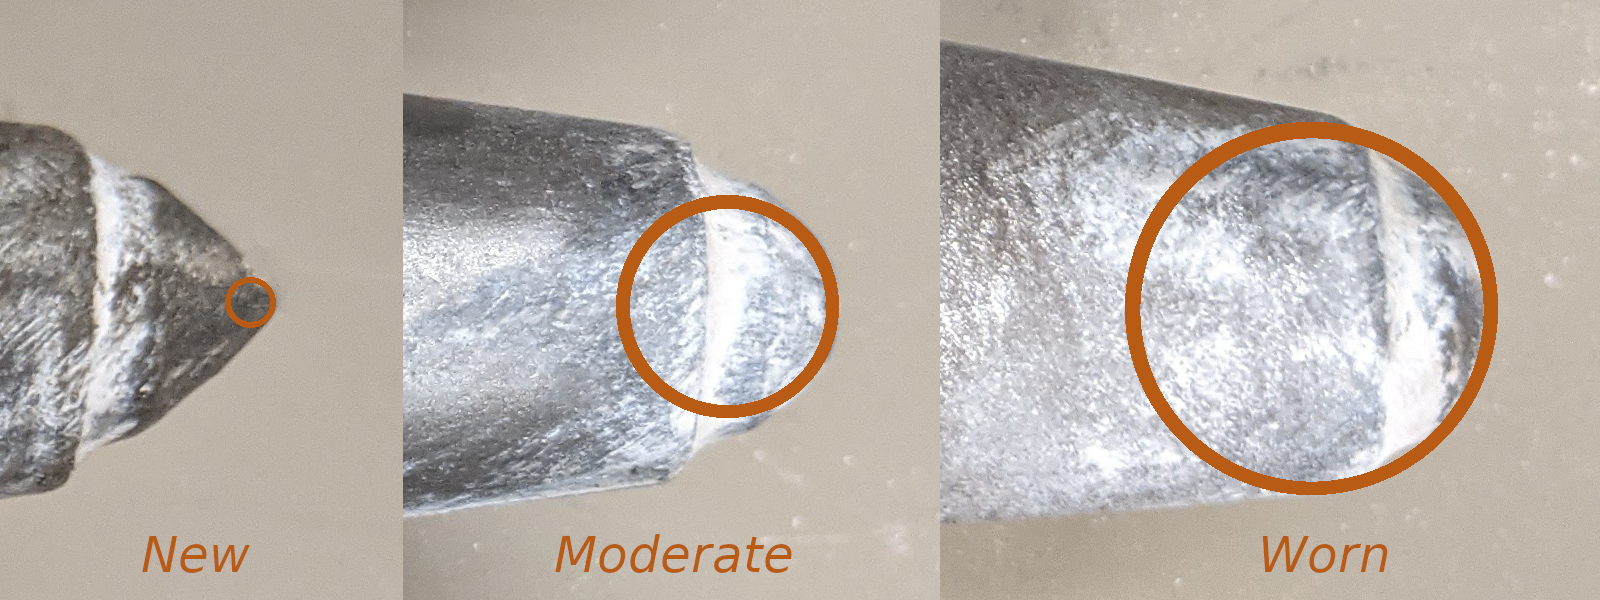
\includegraphics[width=5.5in]{p2_media/figures/tips.png}
\caption{The tips of the conical picks with different wear levels used for the experiment.
The tips are worn to a spherical shape to approximate even wear. The \textit{new} tool is unmodified
and has a diameter of 3.71mm, the \textit{moderately} worn tool has a diameter of 17.9mm,
 and the \textit{worn} tool has a diameter of 27.5mm. The tool tips were artificially worn down using a lathe.}
\label{fig:levels}
\end{figure}

The sample is cut by layers, with each layer consisting of several lines spaced roughly three centimeters apart.
The cutting speed is set to 10 inches per second and penetrations of 1.5 and 2.0 inches are used.
For each wear category, we collected four lines for both penetrations. 
To reduce edge effects of our experiment, 
like the differences in impulse response
between the linear cutting machine and our sensor,
we trim the recording of each line to 6 seconds,
starting shortly after the bit hits the material. 
We chop the data into small segments of 20, 40, 60, 80, 100, and 200 milliseconds in duration.
The segments are allowed to overlap by 50\%, and
this yields roughly 480 samples for the 100 millisecond case and 
4800 samples for the 20 millisecond case for each wear category.

The fast sampling rate of our microphone, 44.1 kHz, means that even short segments,
dozens of milliseconds in duration, will have thousands of data points.
Reducing input dimension via downsampling after low pass filtering will preserve 
low frequency data while leading to faster processing for the classification algorithms and 
eliminate additional aliasing.
These segments also have a Hamming window applied to enforce periodic assumptions of the Fourier based preprocessing.
Longer signal windows will yield more resolution in the frequency domain up to the sampling frequency
while higher sampling rates offer slightly increased resolution but over a wider frequency range.
Our study compares the effect on classification performance from both downsampling and window length.

We score the methods using the F1 score, which penalizes false positives and false negatives,
by generating a distribution of scores and comparing the distributions \cite{Goutte2005}.
We also examine the confusion matrices of the classifiers to understand 
how the classifier is performing \cite{Bramer2007}.
Each window size data set is divided randomly in a 70:30 test train split 40 times 
to collect statistical distributions of the scores for each classification method 
when using a small sample for training data.
The preprocessing and classification methods are described in more detail below.

\subsubsection{Preprocessing}

After filtering, downsampling, and splitting the data into small segments,
the input to each of the classification algorithms is a vector of floating point numbers 
which represents a small segment of the audio recording from the cutting experiment. 
We denote a segment of the data, starting at time $t$, as $\ora{x_t}$.
This vector has consecutive samples of the time domain signal starting at time $t$ and 
ending at the end of the window duration offset by the start time.
The first preprocessing step is to multiply this vector element-wise with a Hamming window, $\ora{h}$, and
the new vector is given as: $\ora{y_t} = \ora{h} \circ \ora{x_t}$.
The exact choice of window function has subtle effects on the algorithm performance, 
but in general the window function serves to enforce the periodic signal assumption of the 
discrete Fourier transform \cite{Harris1978}. 

After the window is applied, the Fourier based preprocessing begins.
The datasets are split 70:30 into the test and train sets. 
We denote the normalized data as $\ora{z_t}$, and it is calculated as:
\begin{align}
\ora{z_t} = (\ora{y_t} - \ora{u}) / \ora{s},
\end{align}
where both subtraction and division are performed element-wise, $\ora{u}$ represents the vector
of mean values for each dimension in the training set, 
and $\ora{s}$ represents the vector of standard deviations for each
dimension in the training set. 
The distributions of frequency spectra magnitudes and time domain waveforms
for each wear category are shown in \ref{fig:natural}.
During each experiment, the test data is normalized according to the distribution of the training set.

\begin{figure}[t!]
\centering
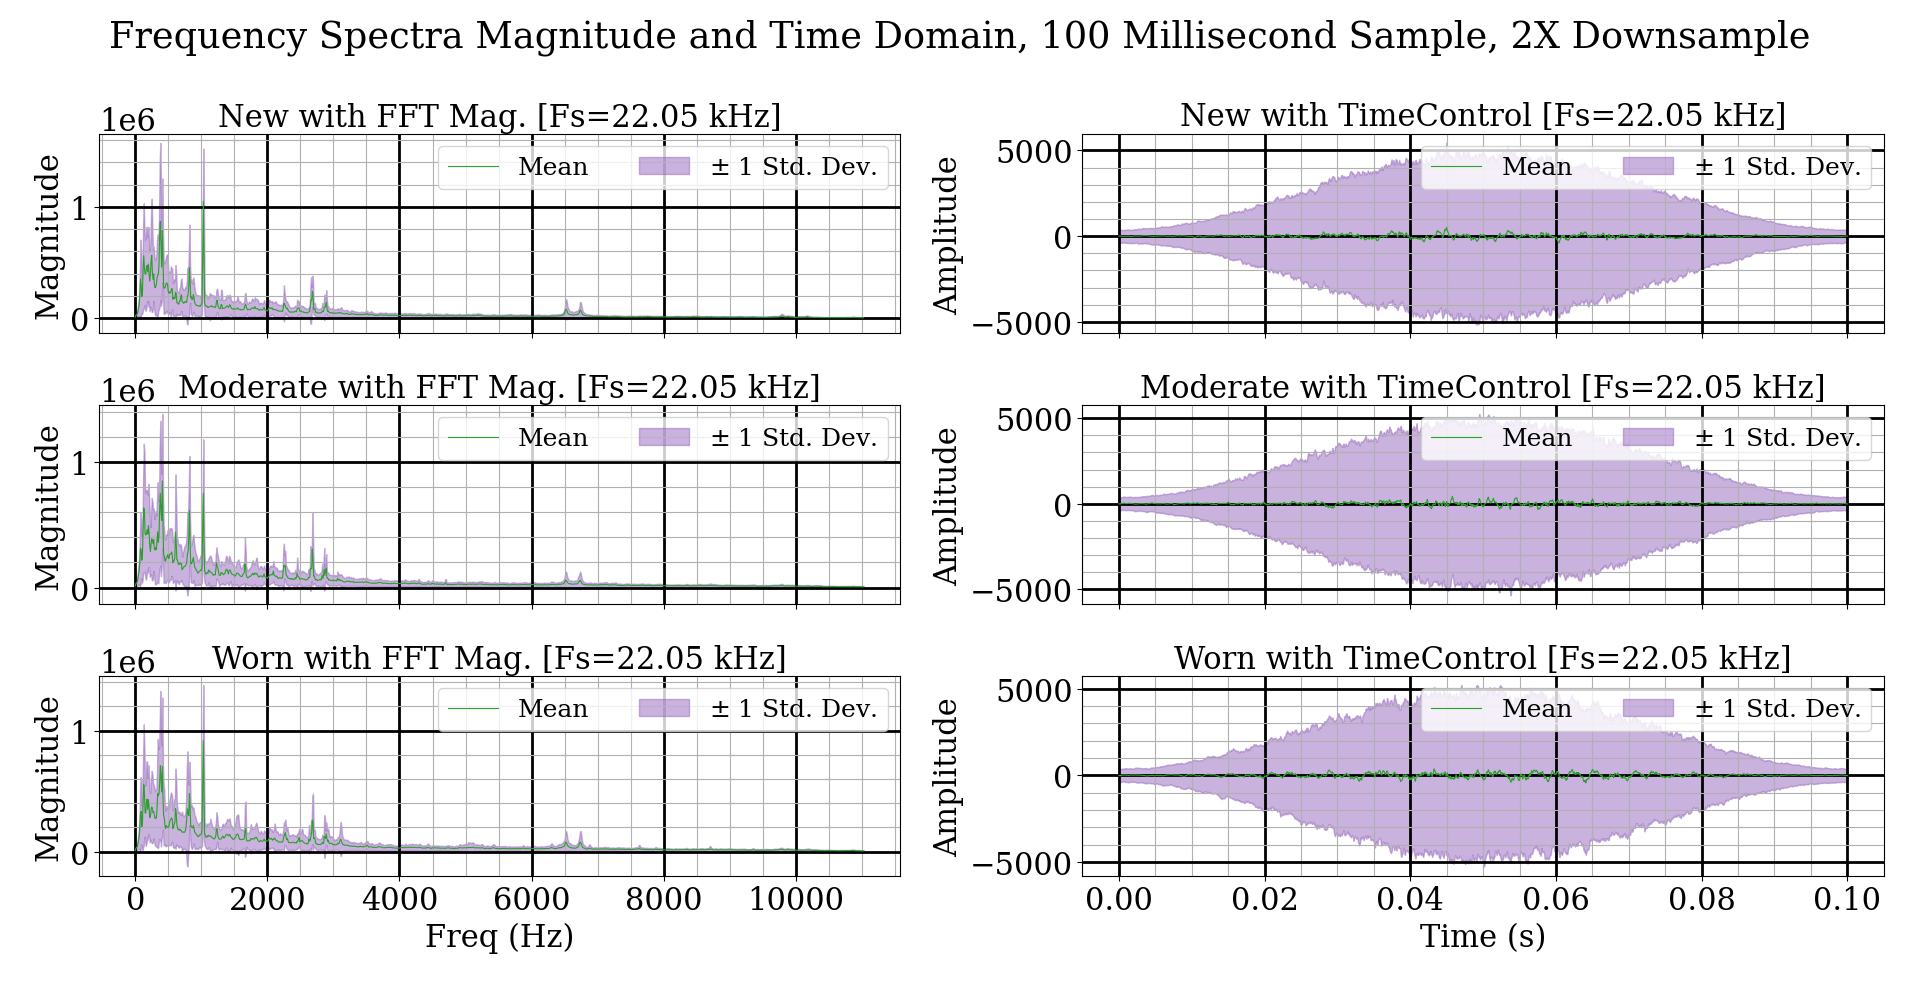
\includegraphics[width=5.5in]{p2_media/figures/raw/fig3_5_natural.png}
\caption{
The natural distribution of frequency spectra magnitude 
and time domain data of each wear category for our collected data.
The Fourier transform data has most of its energy below 4 kHz.
The higher frequency data has smaller variance compared to the
lower frequency data.
The time domain data is roughly shaped like the window function.
Transforming the time domain data into the frequency domain highlights
the changing modes between the categories.
These differences in resonant frequencies are made more apparent after normalization.
}
\label{fig:natural}
\end{figure}

Before invoking any classifiers, we can show here that there are 
objective differences in acoustic spectra across wear categories 
by performing a classic two-sided Welch-Satterthwaite t-test on each frequency bin \cite{Tamhane2000}.
The results of this test and the normalized frequency spectra magnitude distributions
for each wear category are shown in \ref{fig:sigs}.
The classification techniques discussed in the next subsection use these differences to 
determine the wear category of a given sample based on the training data.

\begin{figure}[t!]
\centering
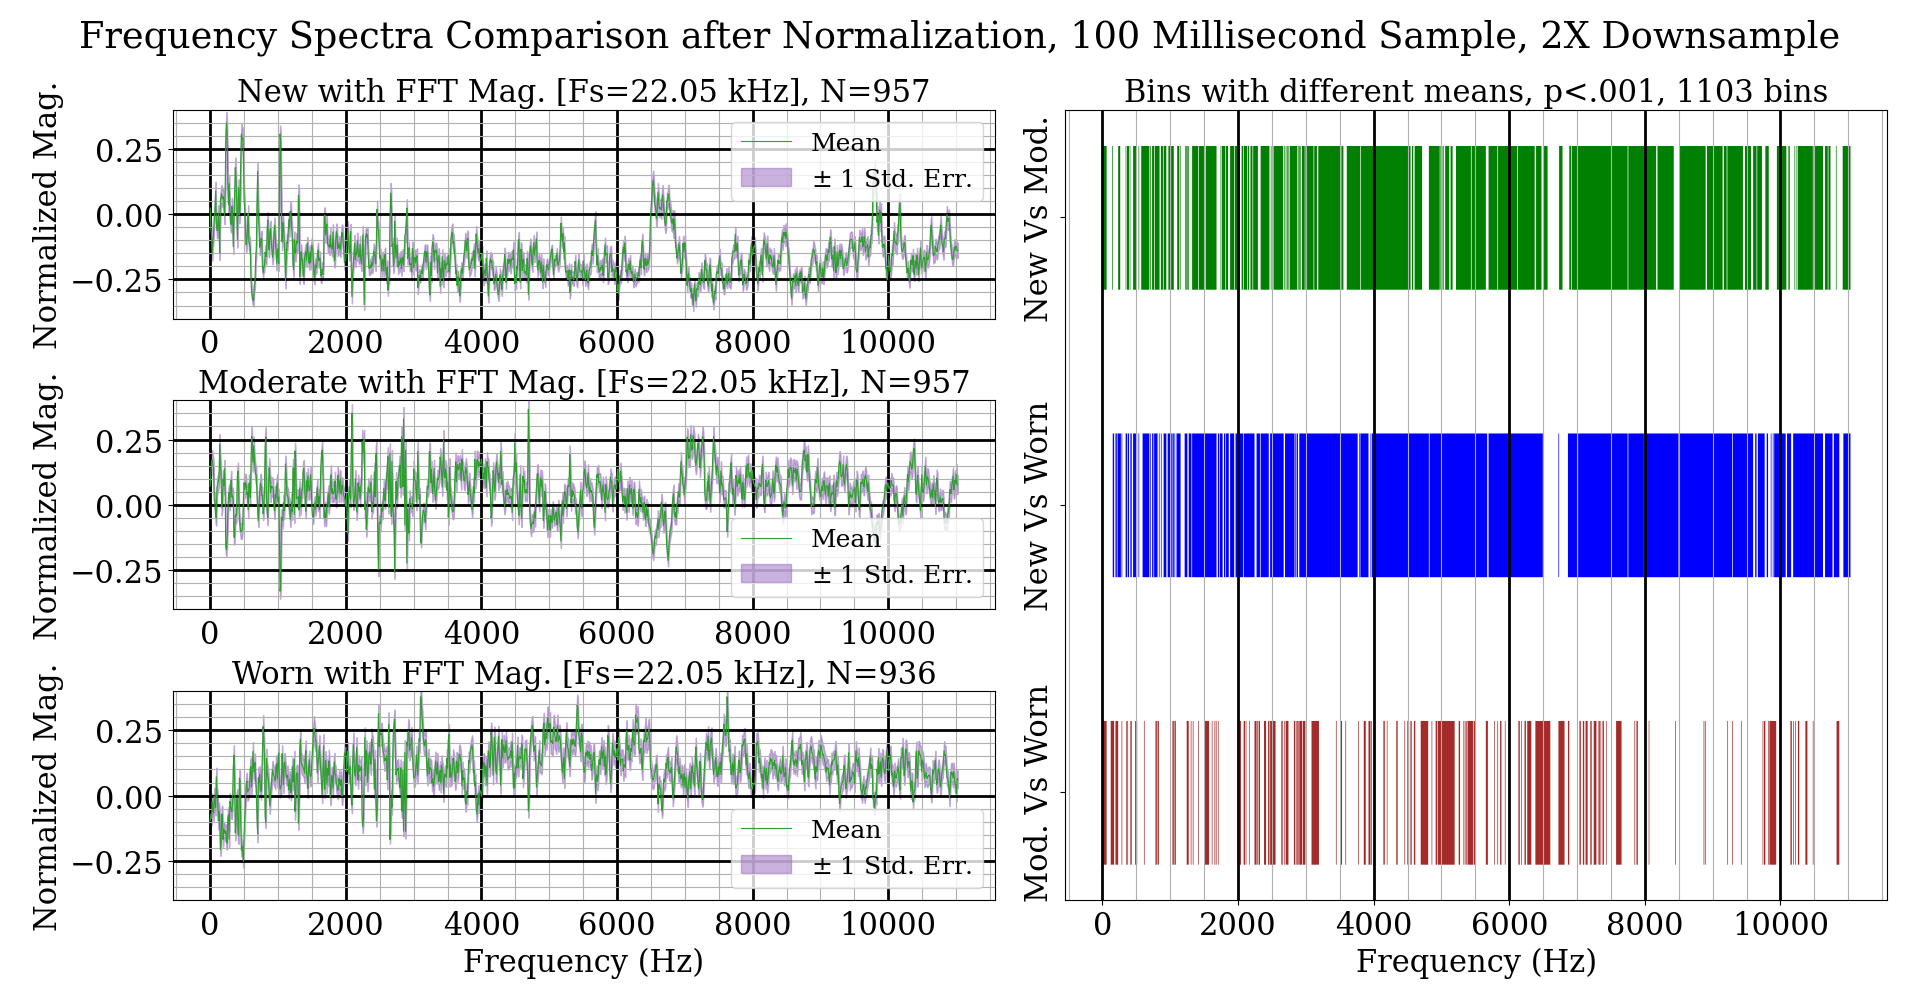
\includegraphics[width=5.5in]{p2_media/figures/raw/fig4_normalized.png}
\caption{
The mean frequency spectra magnitude after normalization for each wear category and a 
comparison between the categories for significant differences.
In the left column, the mean value and the standard error of the mean are shown for our collected data.
In the right column, the results of a t-test for each bin for each pair of categories is shown.
It is known that operators use acoustic signals to determine cutting conditions,
and this figure demonstrates significant, $p < 0.001$, differences across tool wear categories
for most frequency bins. Even though the higher frequencies have less energy, their differences
are still significant due to their low variance.
The exact changes will depend on the machine and the entire set of cutting conditions, but 
for a given environment, these differences can be observed and detected.
}
\label{fig:sigs}
\end{figure}

\subsubsection{Classification}

These data splitting, preprocessing calculations, and classification techniques are 
computed using the scikit-learn, a.k.a. sklearn, library \cite{JMLR:v12:pedregosa11a}.
The library supports many classification and regression methods and facilitates rigorous comparison.
For this study, we choose to compare the support-vector machine technique with a more simple method
and a more sophisticated method to investigate classifier efficiency. 
The more simple method is the k-nearest neighbors classifier.
The k-nearest neighbor technique works by comparing the input sample to its memory of the $k$ closest training samples, 
 and the most popular class is elected as the output.
The more sophisticated method, the multi-layer perceptron classifier, works by training a 
 network of artificial neurons to develop a series of vector transformations which results
 in accurate classification. Meanwhile, the support-vector machine aims to find a separating
 hyperplane in a transformed version of the data. 

To measure the performance of our chosen algorithms, the F1 score is 
used to evaluate the classification results. 
There is an inherent trade-off between precision and recall in practical classifiers \cite{buckland94}.
The F1 score is the geometric average of
precision and recall, and serves to evaluate overall performance. 
More detailed descriptions of the individual classification algorithms follow below.

\subsubsection{K-Nearest Neighbors}

The non-parametric k-nearest neighbors approach is used in classification 
and regression \cite{Vaishnnave12019}.
The K-nearest neighbors classifier aims to predict the class label, $g_t$ of 
future data point $x_0$ on the predetermined $q$ classes given a set 
of $p$ labeled classes $\{(x_t, g_t), t \in 1 \ldots p\}$ \cite{Song2007}. 
In order to obtain the class label for $x_0$, the K-nearest neighbor (KNN)
 classification algorithm searches for the sample's K closest neighbors 
 and then assigns the class of the majority.
The selection of K and the distance measure used are the two factors 
that have the biggest impact on a KNN classifier's performance \cite{Alf2019}. 
Without prior knowledge, Euclidean distances are typically used by the KNN classifier 
as the distance measure. These distances are simple to compute and if the data
categories are distinct, than this method will work well.
We use the Euclidean distance and $K=5$ for this study, with larger values of $K$ giving similar results.

\subsubsection{Support-Vector Machine}

The fundamental goal of the support-vector machine (SVM) is to build a separation hyperplane that best divides
 data examples into two classes while maximizing the minimum distance between points
 and the separation hyperplane \cite{lazarevic2009support}. 
Support-vector machines employ the structural risk minimization \cite{sewell2008structural}
 concept and seek to achieve zero misclassification error while reducing the 
 model's complexity. 
The problem statement and solution of its dual via Karush-Kuhn-Tucker conditions \cite{gordon2012karush}
is omitted here for brevity. 
For discussion, the decision function of the two class support-vector machine is listed here:
\begin{align}
h(x) = \mathrm{sign} \bigg( \sum_{s=1}^p \beta_s g_s k(x_s, x) + r \bigg),
\end{align}
where sign returns 1 if the input is greater than zero, $p$ is the number of support-vectors, 
$\beta_s$ and $g_s$ are weights, and $k(x_s, x)$ is the kernel mapping of the support-vector $x_s$ and the input, $x$, and $r$ is a bias term.
The kernel function is able to compare the input to the chosen support vectors in a space that highlights their differences.

The SVM is a binary classifier by nature, however many of the problems 
we are interested in tackling are multi-class (q-class) \cite{Oskoei08}.
 Hence a multi-class SVM approach must be adopted in that regard. 
In this study, a “one-against-one” approach \cite{Debnath2004} was employed. 
This approach trains q(q-1) binary classifiers to distinguish between two classes. 
The final output is the class that receives the most votes from 
the binary classifiers. 
The coefficients calculated during training are considered optimal for the given data. 
The SVM requires a roughly similar number of computations as the KNN, but takes extra steps to 
make the data more separable through the kernel function.
We use the Radial-Basis function for our kernel, as it is able to make nonlinear separations.

\subsubsection{Multi-layer Perceptron Classifier}
A specific type of feed-forward artificial neural network is the multi-layer perceptron (MLP)
and it is well-known for its stability, usability, and a relatively modest structure 
in tackling some tasks when compared to other structures \cite{yulita2018multi}. 
An MLP classifier analyzes the relationship between input and output 
in a set of p labeled classes. An input layer, a number of hidden layers, and an output layer 
make up the network topology of MLP \cite{molina2021classification}. 
Processing nodes known as neurons make up each layer, 
with each neuron connected to all neurons in the previous layer. 

Each neuron receives weighted inputs with a bias value, which are then 
transformed and processed by a nonlinear activation function \cite{montesinos2022fundamentals}. 
The hidden layer's output is shown in the following:
\begin{align}
s_r = t \bigg( \sum_{q=1}^p \omega_{qr} x_q + c_r \bigg), \quad \forall r \in \{1, \ldots, k\},
\label{eq:layer}
\end{align}
where the activation function is represented by $t(\cdot)$; 
the bias of the $r$th hidden units is represented by $c_r$; 
the inputs and weights between the input and hidden layer are represented 
by $x_q$ and $w_{qr}$, while $s_r$ is the hidden layer's output. 
Activation functions come in a variety of forms, including logistic sigmoid, softmax, 
hyperbolic tangent, and rectified linear unit functions \cite{sharma2017activation}. 
The output layer consists of one neuron for each class, and the output is the
probability that the input belongs to that neurons respective class.

The coefficients for the network are trained in an iterative fashion by examining 
the gradient of performance with respect to each one.
This forward pass and back-propagation process is repeated until the network finds 
a solution or the necessary number of iterations have been completed \cite{maxwell2017deep}.
This type of training requires a balance of many factors to be successful; but once trained,
the network can classify samples with a roughly similar number of computations as the other
techniques depending on the network size.
We use the rectified linear unit activation function and a network of two hidden layers 
equal in size to the input dimension, with more hidden layers giving similar results.

\subsection{Results}

The mean F1 scores are plotted against the window lengths for each of the tested methods 
at each of the tested downsampling factors.
The K-nearest neighbors classifier performance is shown in \ref{fig:perf_KNN}.
The support-vector machine classifier performance is shown in \ref{fig:perf_SVM}.
The multi-layer perceptron classifier performance is shown in \ref{fig:perf_MLP}.
In the above figures, the F1 score of a method is significantly greater than another method
if the median score is above the max score of the other method.
This comparison method is slightly more conservative but more visually straightforward
than comparing each score in the collected distribution,
as recommended in \cite{Goutte2005}.
Classifier performance was greater with longer window lengths and 
increased sampling rates, or lower downsampling factors.

Looking at the confusion matrices for the different types of classifiers generally showed
that most of the confusion was between the \textit{moderate} and \textit{worn} categories of bits, suggesting that
these two categories have responses that are more similar to each other than to the \textit{new} category.
A sample confusion matrix for a SVM classifier experiment is shown in \ref{tab:conf}, 
it is representative of most of the other classifiers too. 
It shows that there is about twice at much confusion between \textit{moderate} and \textit{worn} categories as there is 
between \textit{new} and the other two wear categories.
This indicates that determining wear to a fine degree may be difficult with acoustic emissions alone.

\begin{table}[h]
\centering
\caption{Confusion Matrix for Acoustic Wear Classifier; Normalized by true class size. \newline
         Concrete sample, 100 millisecond window, 70:30 test train split, \newline
         support-vector machine with fast Fourier transform preprocessing.}
\label{tab:conf}
\begin{tabular}{|l|lll|}
\hline
Test Result \% & \multicolumn{3}{l|}{Prediction}                            \\ \hline
True Class    & \multicolumn{1}{l|}{\textit{new}} & \multicolumn{1}{l|}{\textit{mod}} & \textit{worn} \\ \hline
\textit{new}           & \multicolumn{1}{l|}{90.15 }    & \multicolumn{1}{l|}{ 4.77}    &  5.08    \\ \hline
\textit{mod.}           & \multicolumn{1}{l|}{3.85}    & \multicolumn{1}{l|}{87.26}    &   8.89    \\ \hline
\textit{worn}          & \multicolumn{1}{l|}{5.67}    & \multicolumn{1}{l|}{9.25}    &  85.07     \\ \hline
\end{tabular}
\end{table}

%array([[0.90153846, 0.04769231, 0.05076923],
%       [0.03851852, 0.87259259, 0.08888889],
%       [0.05671642, 0.09253731, 0.85074627]]), 

%\caption{Confusion Matrix for Acoustic Wear Classifier; Normalized by prediction \newline
%         Concrete Sample, 100 millisecond Window, 70:30 test and train, SVM with FFT_Mag.}
%\begin{tabular}{l|c[table-format=2.2]c[table-format=2.2]c[table-format=2.2]|}
%{Test result \%}   & \multicolumn{3}{l|}{Prediction}                 \\ \hline
%{True Class} & \multicolumn{1}{l|}{\textit{new}} & \multicolumn{1}{l|}{\textit{mod.}} & {\textit{worn}}  \\ \hline
%{\textit{new}}        & 90.15                   & 4.77                     & 5.08 \\
%{\textit{mod.}}       & 3.85                    & 87.26                    & 8.89 \\
%{\textit{worn}}       & 5.67                    & 9.25                     & 85.07
%\end{tabular}
%\end{table}

\begin{figure}[t!]
\centering
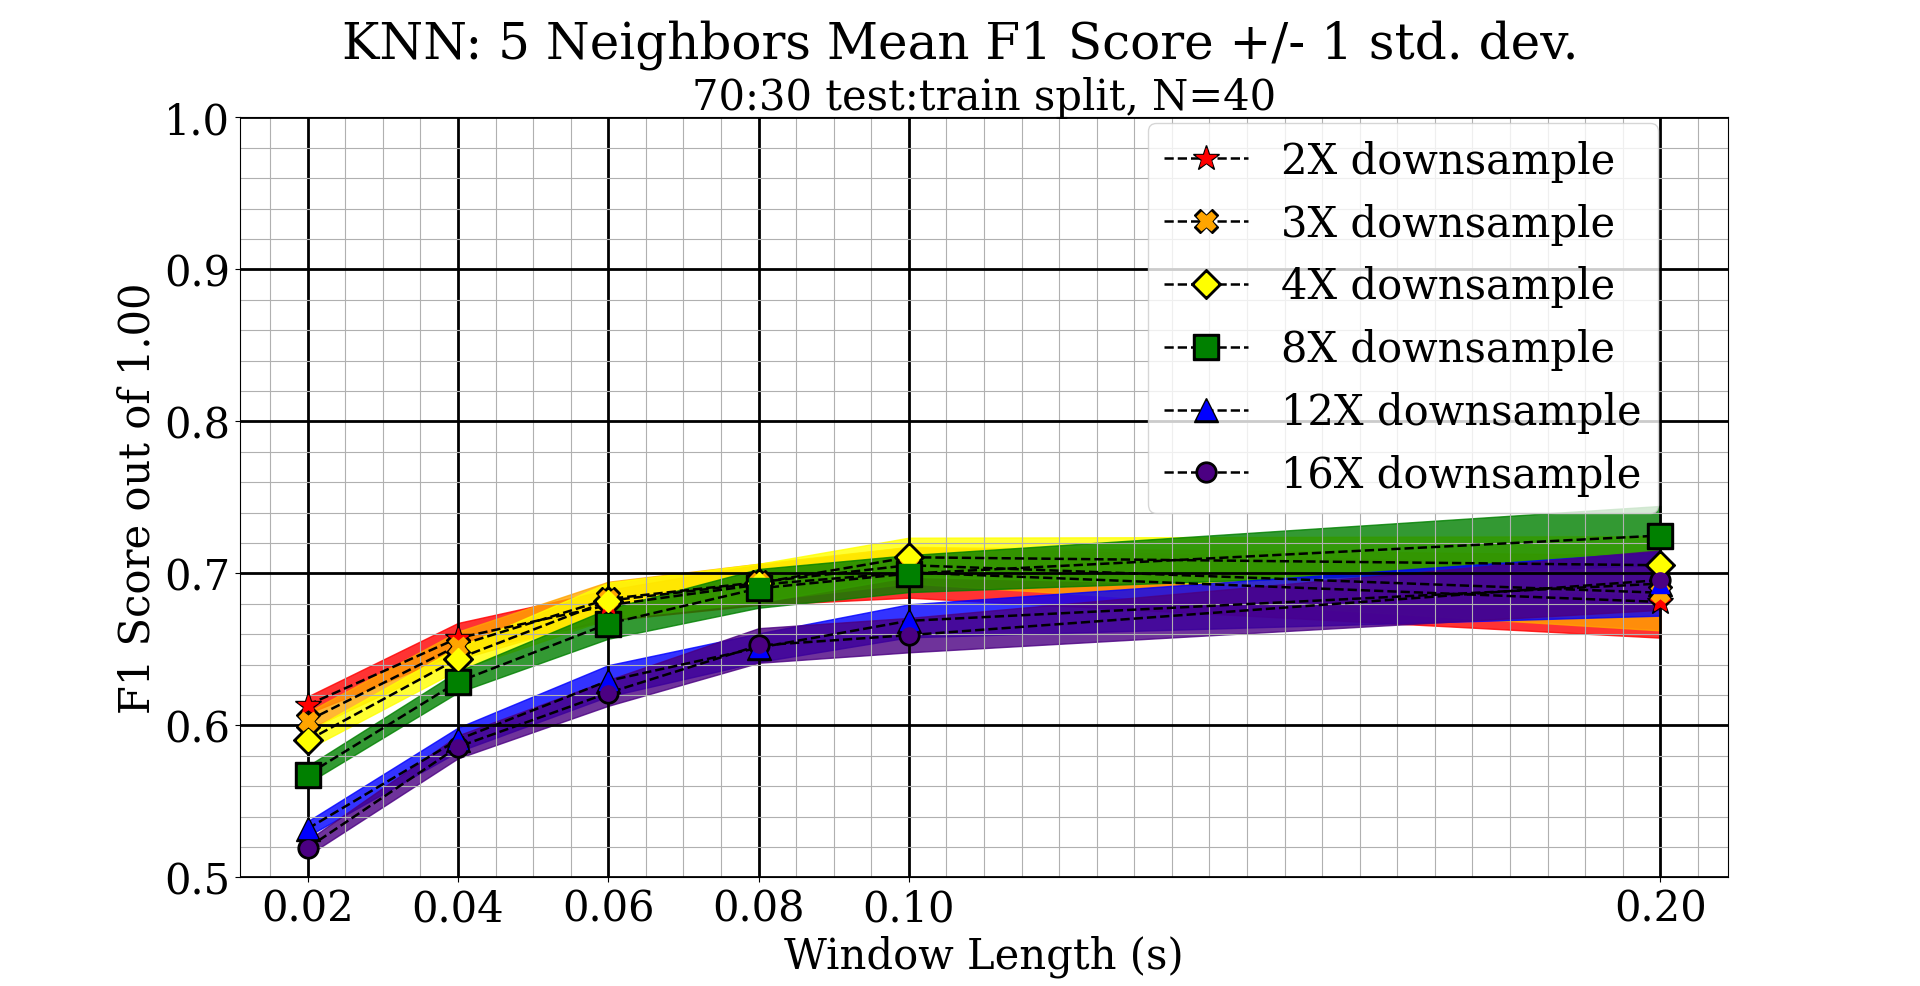
\includegraphics[width=5.5in]{p2_media/figures/raw/KNN_F1_scores.png}
\caption{The mean F1 score and standard deviation for K-nearest neighbors method. 
Using K=5 gave slightly better performance than other values, 
but this method performed the worst overall.
Increasing window length gave better performance for this method, and downsampling had little effect
for larger window lengths. 
The F1 score only increased a small amount when using the 0.2 second window compared to the 0.1 second window.
}
\label{fig:perf_KNN}
\end{figure}

\begin{figure}[t!]
\centering
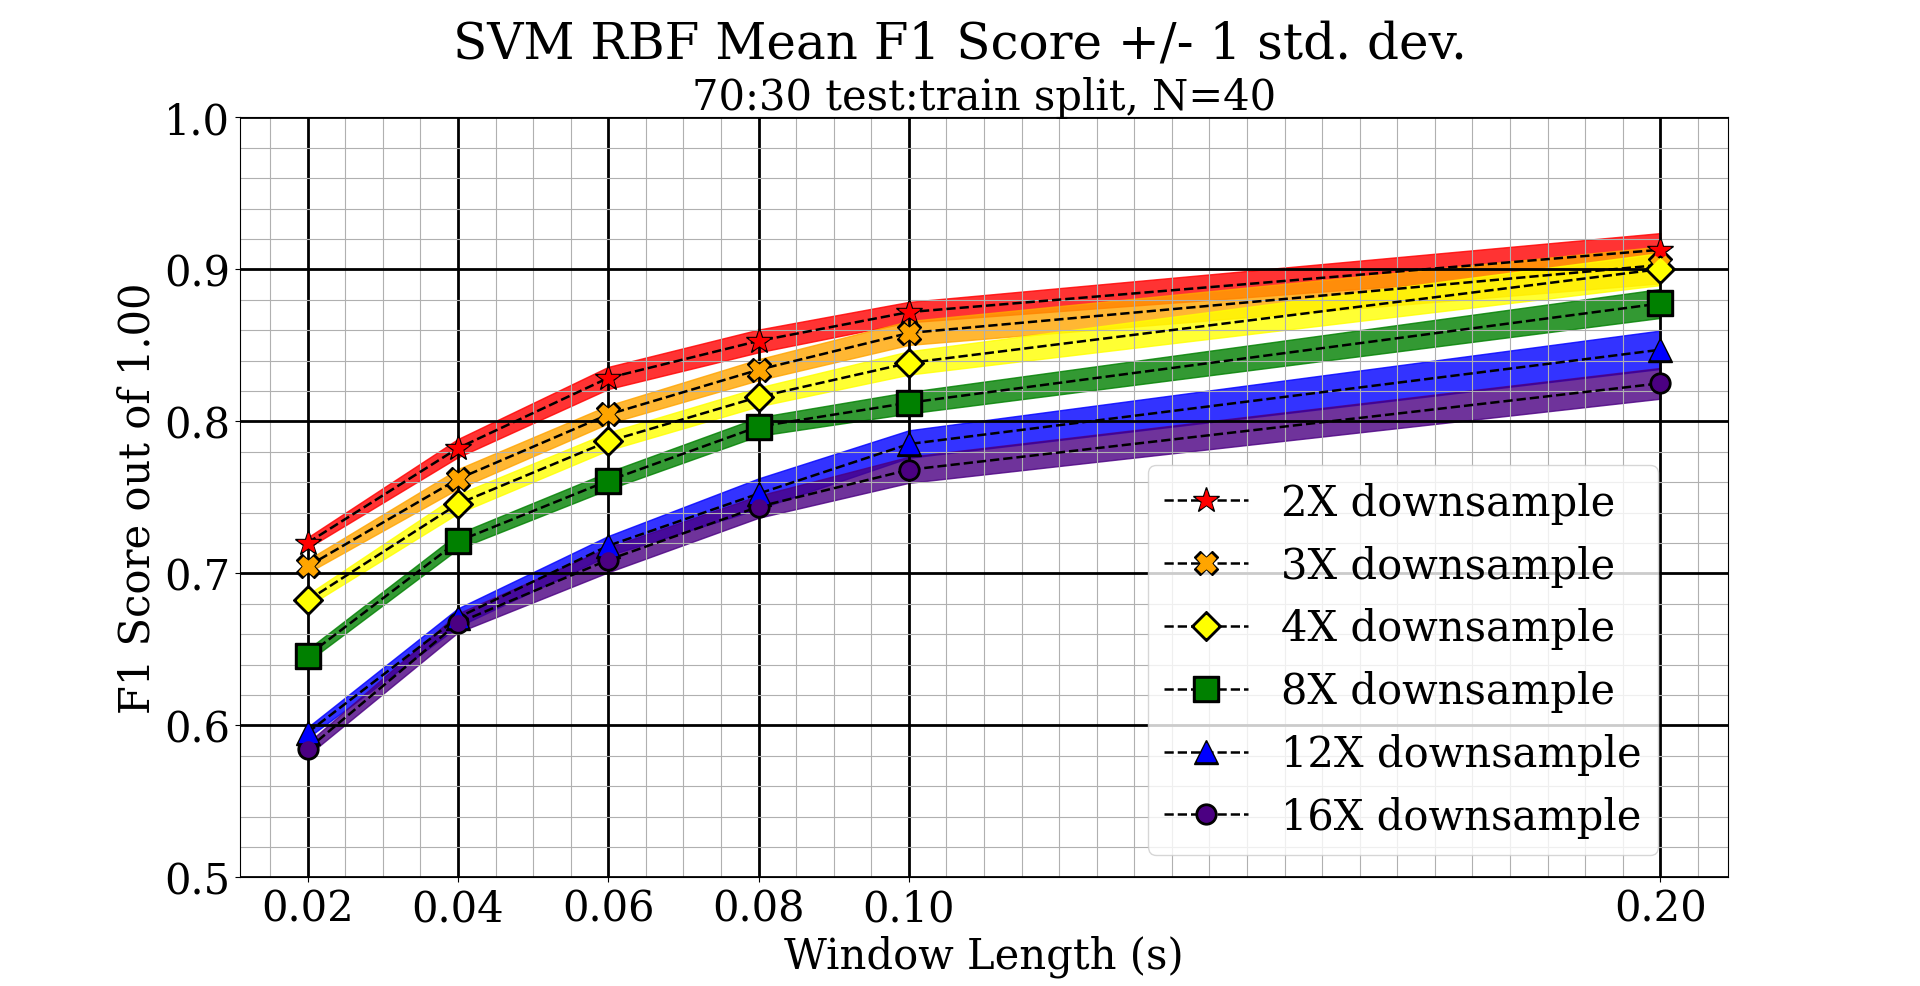
\includegraphics[width=5.5in]{p2_media/figures/raw/SVM_F1_scores.png}
\caption{The mean F1 score and standard deviation for the tested support-vector machine method.
This is a low hyperparameter method that performs very well and does so efficiently.
With this method, performance trends better with longer window length 
and higher sampling rates, or less downsampling, for our experiment.
Increasing window length gave better performance for the number of variables introduced
compared to increasing sampling rates.
Using a window length of 0.2 seconds gave the best performance of for all downsampling levels,
and the performance was similar for samples with less downsampling.
}
\label{fig:perf_SVM}
\end{figure}

\begin{figure}[t!]
\centering
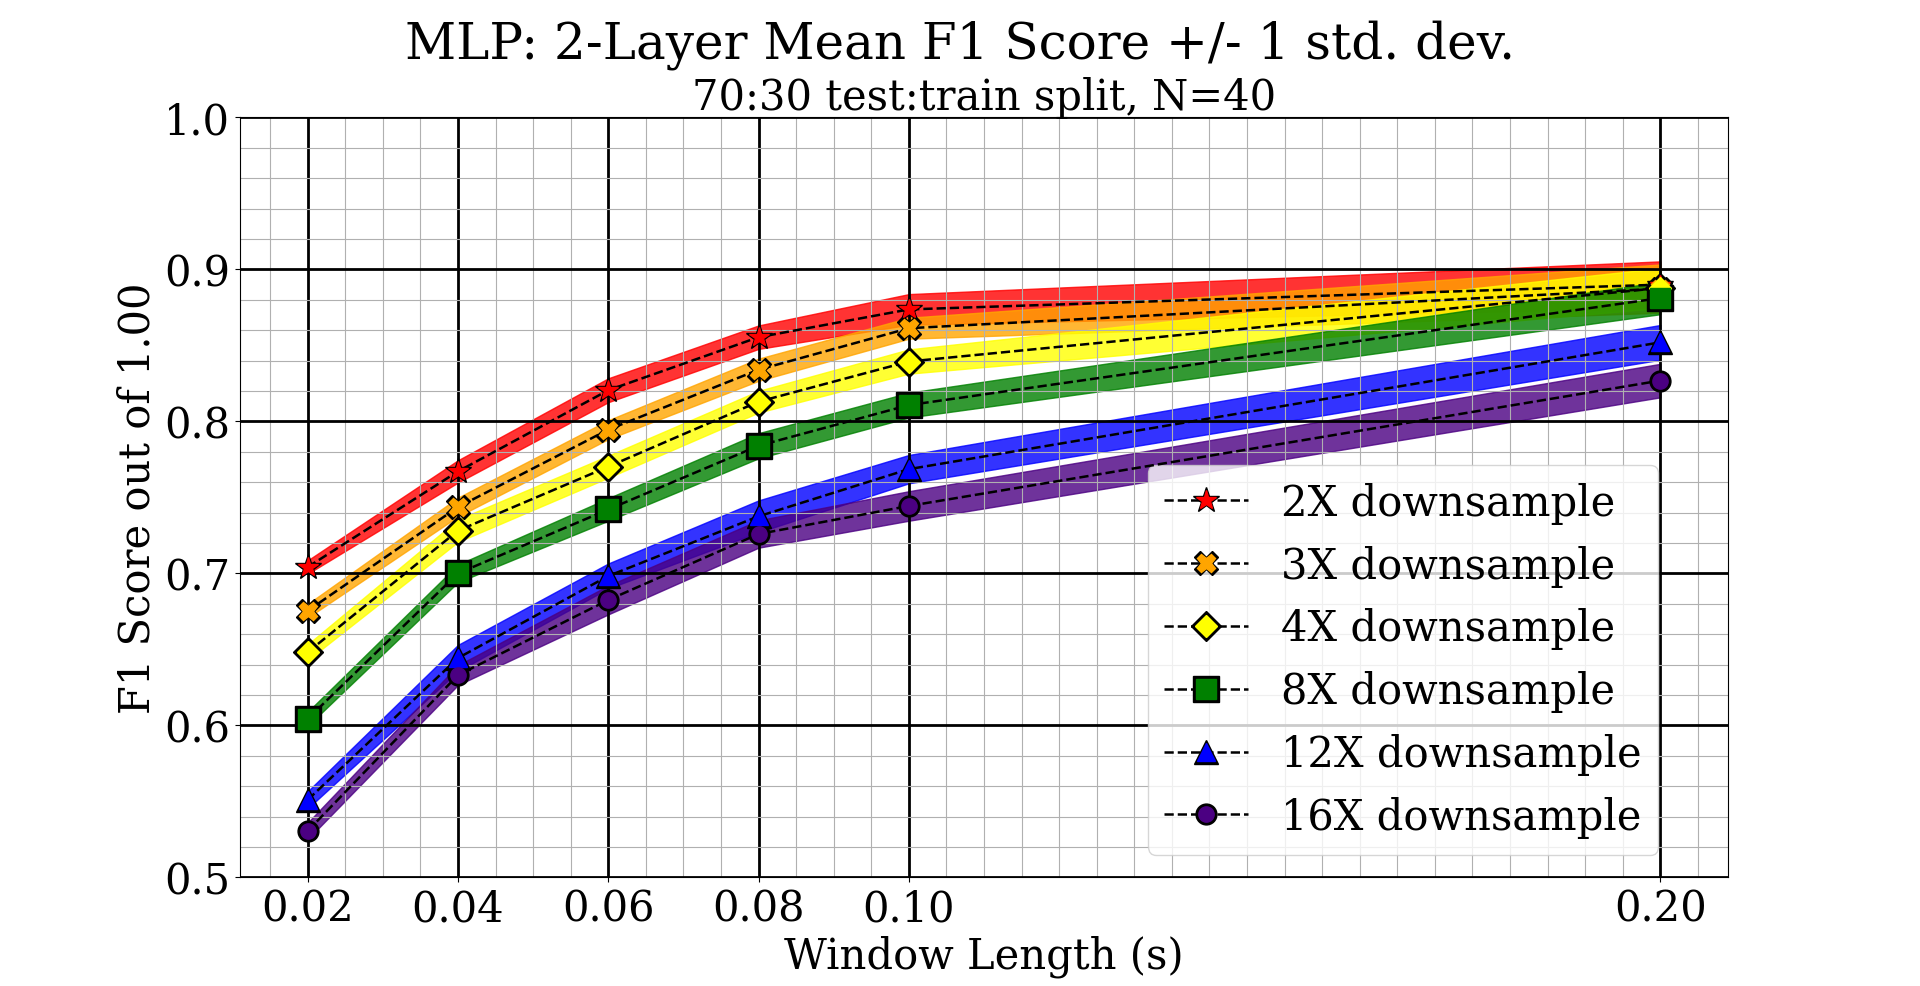
\includegraphics[width=5.5in]{p2_media/figures/raw/MLP_F1_scores.png}
\caption{
The mean F1 score and standard deviation for the tested multi-layer perceptron methods.
This method has the power to classify data very accurately for samples similar to its training data.
Different network sizes are tested to achieve maximum performance.
This method scores similarly to the support-vector machine, but uses more resources.
Both longer window lengths and higher sampling rates, or less downsampling, increased performance.
Increasing window length gave better performance for the number of variables introduced
compared to increasing sampling rates.
Using a window length of 0.2 seconds gave the best performance of for all downsampling levels,
and the score tapered to about 0.90.
}
\label{fig:perf_MLP}
\end{figure}


\subsection{Discussion}

It is well known that changes in tool wear produce changes in vibrational response
across many domains. This fact is also true in the case of underground mining. 
Human operators use sound cues as one of the means of assessing tool wear during operation.
The operators have many duties, and this skill can be difficult to train, 
since the process is subjective. By providing operators a means to perform some of these
duties from a safer position, their exposure to risks at the mining interface can be reduced
\cite{Bartels2009}. 
We propose the addition of objective acoustic data collection and analysis to aid in tool wear classification.

When using methods like the ones described in this work, the cutting conditions must be taken into account.
For example, cutting different materials can also produce different modal responses as well as cutting
at different speeds, penetrations, and with different tool geometries. The operators ability to deduce
changes in wear in different materials comes from experience in cutting those materials with tools at 
different wear levels. Likewise, to successfully apply this technique, data would need to be captured
and analyzed for different cutting conditions.

When comparing the methods for implementation in the application, the support-vector machine
would be an efficient classifier to use, as it scores as well as the multi-layer perceptron classifier,
but has reduced computational complexity. Our results also indicate that longer sample times, which 
give increased resolution for the sampled frequencies, provides better classification performance than
using an increased sampling rate for a shorter duration considering the number of variables introduced.
%This effect continued even with longer sample duration and greater downsampling rates than presented here.

With a window of 0.2 seconds, the tested sampling rates had similar performance.
At this sample length, the input dimension is large, especially when little downsampling is used.
Use of larger samples was computationally infeasible for our equipment and 
also would also have reduced the number of samples available in our data set.
The good performance of signals with long duration and downsampling
implies that lower frequencies are of particular interest for tool wear classification in rock cutting.
The code and data used for this work are available at:
\url{https://github.com/Fworg64/concrete_tool_wear}.

After classification, human operators could be alerted to the anomalous conditions 
to allow them to make a decision to either stop the operation
for further diagnostics or continue cutting if they know from experience 
what could be causing a false positive or how long to extend the current operation.
Also, this technology that can monitor tool wear in an objective manner
would provide a mechanism to monitor the performance of human operators. 
This can help operators and other stakeholders identify areas where they can improve.
It can also be used to assist in training and help to identify risky operation.
Either way, the feedback could be collected from a greater distance, 
reducing the operators exposure to dust and other hazards.

To implement this technology, only a simple and low-cost microphone would need to be placed near
the cutting interface to detect the mode shifts associated with changing tool wear. These devices
are low power, low cost, and very portable, making them well suited for the mining environment.
However, since the signal is only collected from one or maybe several points, it is unlikely that
this technology could predict which tools are worn on the drum head. Also, interference from nearby
operations which are producing noise could also affect the accuracy of this method were it to be
deployed to an active mine. Ultimately, this technology could assist operators in performing their
role from a greater distance and provide a level of objective feedback that is not currently present.


\subsection{Conclusion}\label{sec13}

In this paper, we showed a method for classifying the different acoustic signals
generated by conical picks of different wear levels cutting into a controlled concrete sample. 
The changes in tool mass and geometry lead to excitation of different modes,
which can be detected and classified by the tested methods after 
appropriate preprocessing. Of the tested methods,
the support-vector machine using long duration samples that are downsampled to an appropriate dimension, 
like 200 milliseconds and 4 times downsampling,
performs well and is computationally efficient.

Acoustic emissions are currently processed by human operators with many duties. 
By automatically classifying the acoustic emissions, operators
can be enabled to perform their role from a greater distance.
This way they can avoid hearing damage, harmful dust, and machine proximity
while being able to focus on their many other duties.
With sufficient data collection, 
this classification can be performed with a microphone and an embedded processor.


%\backmatter

\subsection{Acknowledgments}

Special thanks to AliseH and Tivali24 for contributions to the python code for running the experiments
and displaying the data. Special thanks to Syd Slouka for helping run the experiments 
and to Carson Malpass for helping design mounts for acoustic sensors. 

\subsection*{Declarations}

\subsubsection*{Funding}
This work was funded by NIOSH Contract
75D30119C05413, “IMPROVING HEALTH AND SAFETY OF
MINING OPERATIONS THROUGH DEVELOPMENT OF THE
SMART BIT CONCEPT FOR AUTOMATION OF MECHANICAL
ROCK EXCAVATION UNITS AND DUST MITIGATION.”

\subsubsection*{Conflict of interest}
The authors declare that there is no conflict of interest.

\subsubsection*{Availability of data and materials}
The data used for this research is available publicly at: \\
\url{https://github.com/Fworg64/concrete_tool_wear}

\subsubsection*{Code availability }
The code used for this research is available publicly at: \\
\url{https://github.com/Fworg64/concrete_tool_wear}

%%===========================================================================================%%
%% If you are submitting to one of the Nature Portfolio journals, using the eJP submission   %%
%% system, please include the references within the manuscript file itself. You may do this  %%
%% by copying the reference list from your .bbl file, paste it into the main manuscript .tex %%
%% file, and delete the associated \verb+\bibliography+ commands.                            %%
%%===========================================================================================%%

%\bibliography{sn-bibliography}% common bib file

\chapter{This is the title of a paper included in a thesis
\label{chap:P3}}

\begin{center}
    Reproduced with the permission for The Journal of ABC. \thefootnote[1]{text}
    
    Jane Jones, Sam Smith, Ann Adams
\end{center}

\subsection{Abstract}

This is the abstract that is part of the paper. If the abstract does not completely fill the page, the introduction also starts on this page. There are no page breaks between the different sections within the paper.

\subsection{Introduction}

The text of the introduction starts on the same page as the abstract, as long as there is room for at least two lines of text beneath the heading (This \LaTeX{} template should look for this automatically.) The headings within this chapter will match the style used in the rest of the thesis. All pages of text within the paper are completely filled in.

The next chapter shows another example with some foot notes for the authors, and the permission form the journal. Here is another quick sentence to make this paragraph look longer than it actually is, and not adding any new information for you to use.

% Extra Example Chapters If you want to See Special Cases with Table, Figure, or Equation formatting
\chapter{Load cell design comparison
\label{chap:8}}

Over the course of this program, two primary load cell designs were tested.
The first design had two electrodes separated by a thin, 25 $\mu$m, layer of polyimide.
The second design had a single electrode coated in soldermask 
and attached to a thicker, 100 $\mu$m, layer of polyimide.
Both designs were tested in a load frame prior to rock cutting use,
and comparable XY plots are shown for both the first and second design
in \ref{fig:xycompare}. The first design is the ``Dynamic Flex Configuration'' 
and the second is the ``Air Gap Configuration''.

The first design was already very thin when it when into the rock cutting test.
The nonlinear deformation characteristics of the thin film made it difficult to determine
cutting forces, but still allowed frequency analysis for determining material type and tool wear.
The second design ultimately altered to the ``Crushed Gap Configuration'' when used for rock cutting.
This final form had even greater sensitivity and linearity, which allowed estimation of cutting forces.

Measurements for individual sensor channels and the measured 
and estimated forces are shown in \ref{fig:sense_chans}.
When attempting to estimate the rock cutting forces to determine material type and tool wear, 
the problem can be relaxed to estimating average cutting force, as the differences in 
cutting force between the conditions are great.
The cutting force bandwidth was limited to 10 Hz for the study, as this is believed to still
provide an adequate response time while providing good averaging.

Force on the cutting tool is determined by the tool geometry and the material.
The force is also influenced by the dynamics of the machine.
The physical sensor system also has dynamics, and depending on the model, 
these dynamics can be non-stationary.
The first design that was tested had non-linear, non-stationary dynamics.
The second design was more linear and the bias could be tracked and compensated.

The air gap design could work for applications with more gentle load profiles,
but considering that the gap will be crushed when exposed to rock cutting forces 
means that this aspect of the design is unnecessary. The first sensor design
has a high bandwidth due to its thin film. 
High bandwidth sensing is good for frequency analysis methods.
More linear and robust sensors are generally bulkier, but at the cost of sensitivity.
By starting with a thick polyimide film and allowing it to be compressed during the application,
we get a robust sensor that is stiffer and more sensitive than the original design.


\begin{figure}[ht]
\centering
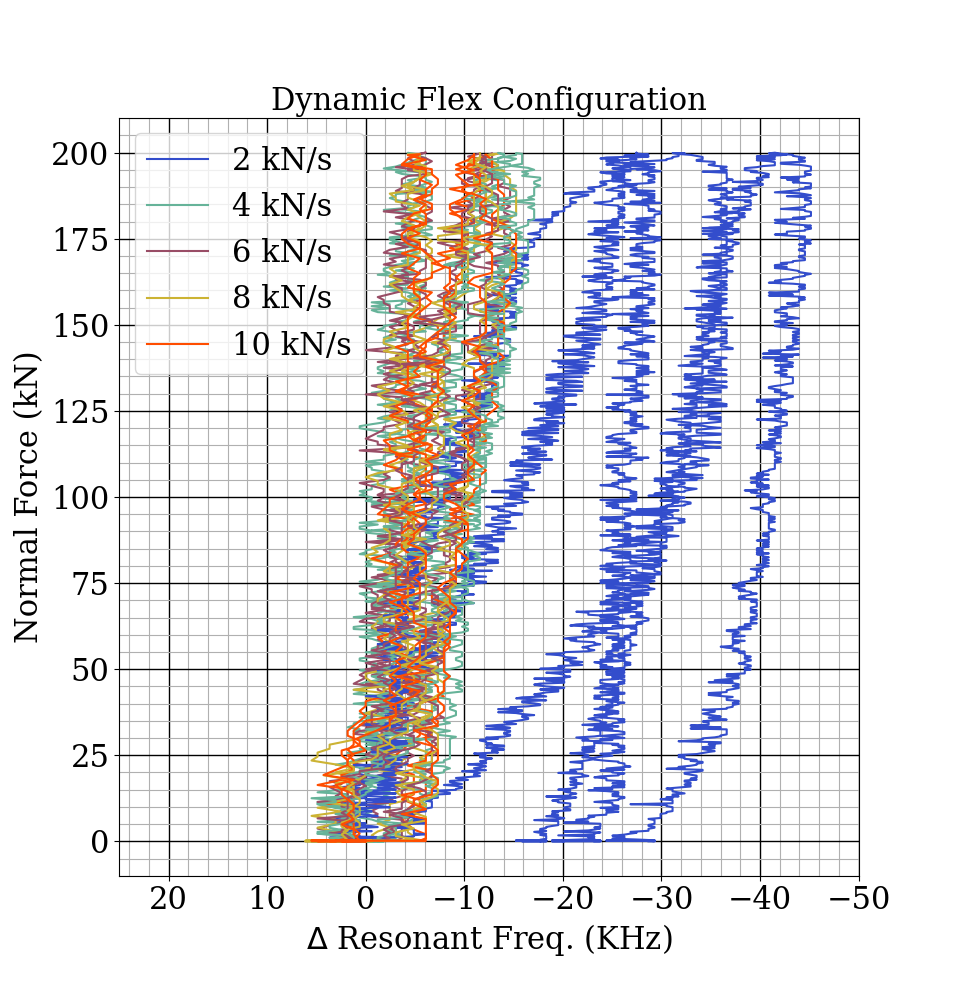
\includegraphics[width=3.0in]{ch8_flexcell.png}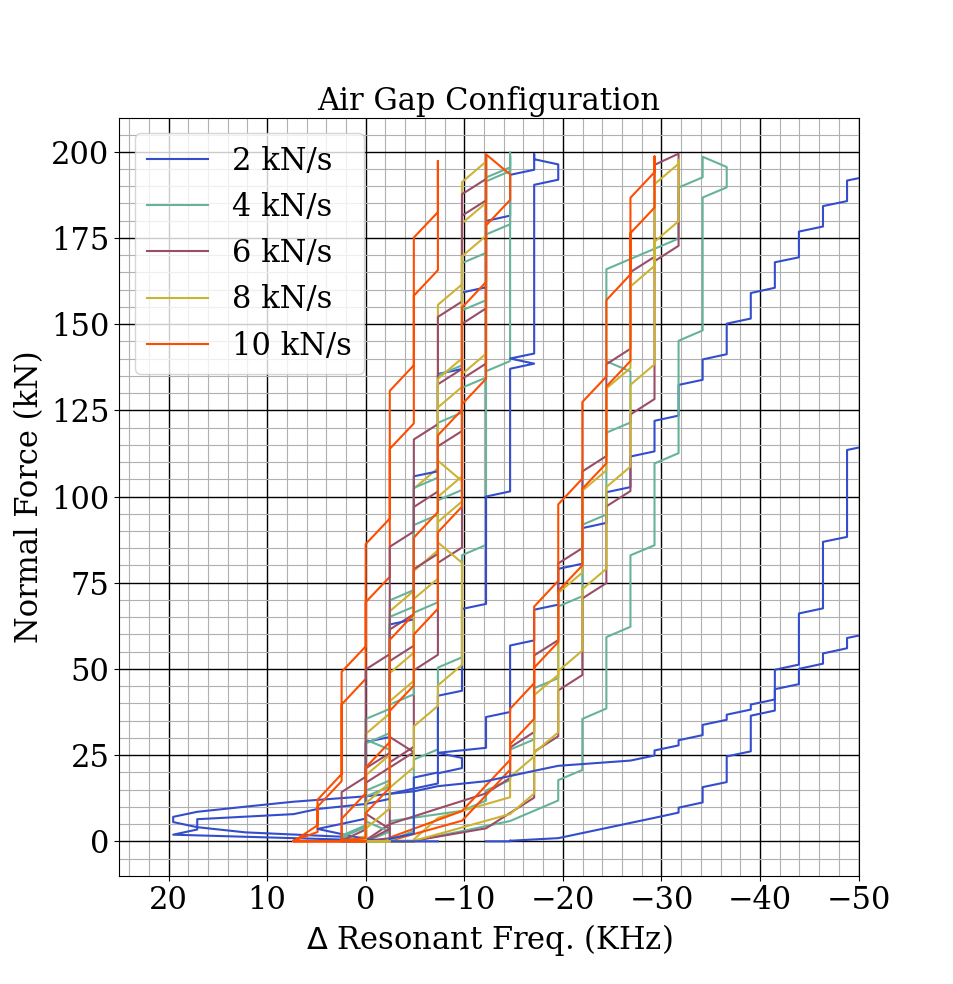
\includegraphics[width=3.0in]{ch8_airgap.png}
\caption{
Comparison of original design, left, and improved design, right.
The original design was noisy, had slightly less initial plastic deformation,
and similar sensitivity when compared to the improved ``Air Gap Configuration''.
The air gap design had much better repeatability and less hysteresis in comparison 
to the original.
The air gap design ultimately became more sensitive when used in the rock cutting tests.
}
\label{fig:xycompare}
\end{figure}



\begin{figure}[h]
\centering
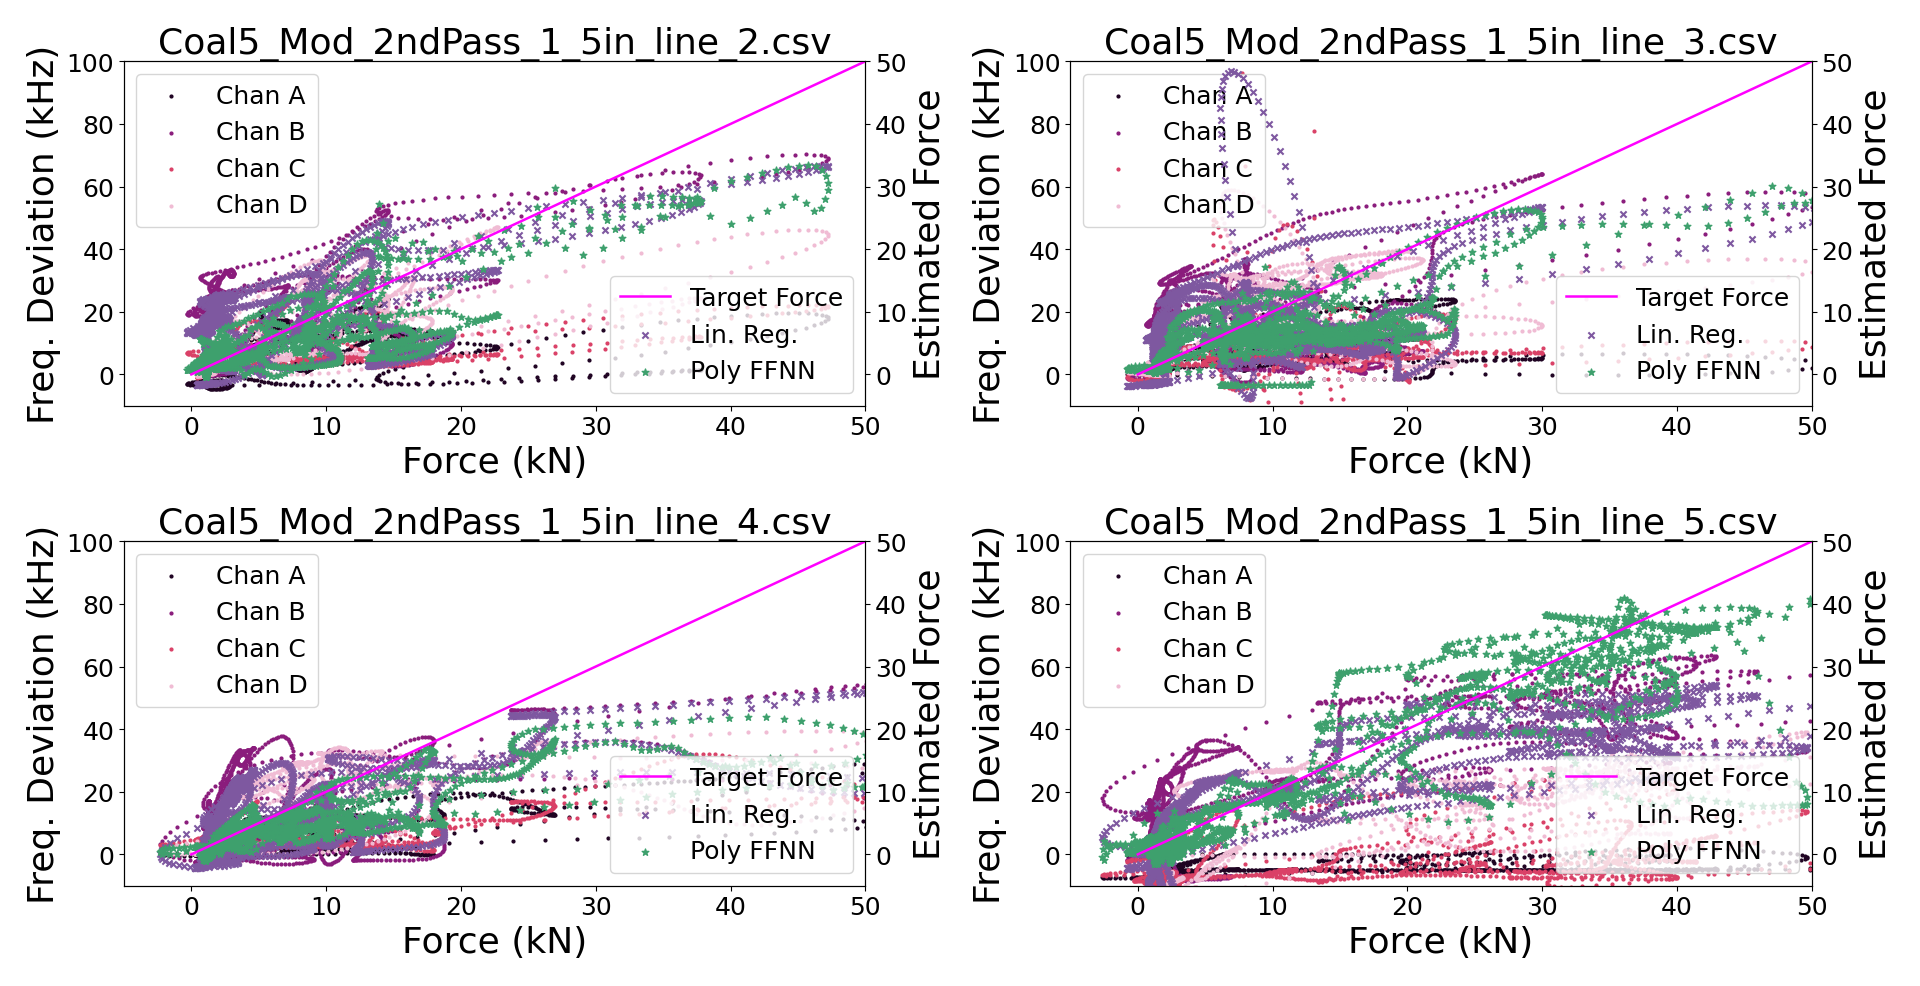
\includegraphics[width=5.5in]{ch8_sense_vals.png}
\caption{
The individual channel measurements and the resulting force predictions for a few choice cuts,
using the ``Crushed Gap Configuration'' of the second sensor design.
The change in resonant frequency from the initial value is plotted versus the target force
for each sensing channel in the sensor. The resulting force estimate provided by both the 
linear regression and the neural network using the 2nd order polynomial expansion are shown.
Ideal performance is shown along the magenta line. 
The neural network method is able to untangle some of the non-linearity in the response.
The performance of the neural network is comparable to the strictly linear model.
The sensor is not completely linear, but can still provide useful measurements using a linear model.
}
\label{fig:sense_chans}
\end{figure}

 % comparison of p1 and p3
\chapter{Longer downsampling rates for acoustic classification
\label{chap:acoustic_extension}}

The effect of increased sample length and downsampling

The effect of different frequency preprocessing methods

The effect of different window shapes

 % further results from p2
\chapter{Sensor Linearity
\label{chap:10}}

To map the crushed gap sensor measurements to estimated forces, 
a regression to the forces as measured by the 
Linear Cutting Machine's strain gauges was used.
This method has a few limitations, the most significant
being the distance between the tested sensor and the strain gauges.
Because of the distance, the higher frequency force components will
be out of phase when compared. 
In addition to the distance, the viscous nature of the polyimide dielectric distorts the 
frequency response when the two measurements are compared.
The electronics for the sensor also contribute high frequency noise to the measurement.
For these reasons, the higher frequency components of the force are not directly correlated 
between the two systems. 
A plot of the transfer function between the measurements is shown in \ref{fig:sense_tf}.

The final sensor prototypes are shown in \ref{fig:airgap}.
When it comes to integrating this sensor with the target application,
construction of the sensor contributes to overall linear performance.
The steel case is assembled using the laser weld procedure described in \ref{app:laser}.
Simulation for the capacitance of the air gap is described in \ref{app:sim}.

The capacitive steel donut with viscous polyimide filling is a useful base design
for many robotic applications. Robustness, linearity, and sensitivity are important 
parameters for any sensor design. Ways to improve each of these categories is listed in \ref{tab:improve}.
To overcome the conflicting directions between sensitivity and the other design goals,
 use a thicker film and compress it down so that it becomes more thin and stiff.
Based on the other results in this work, high frequency classification 
should also be considered a valid method for
 determining material type and tool wear. 
Directly embedding a piezo element within the tool could
also serve to measure higher frequency vibrations which vary with cutting parameters.
Future works may be able to integrate the sensing membrane with the cutting tool,
using the tool to protect the sensor while it measures vibrations or cutting forces.


\begin{table}[]
\centering
\caption{Changes to design parameters that would improve certain categories}
\label{tab:improve}
\begin{tabular}{|r|c|c|c|}
\hline
Parameter               & Robustness   & Linearity    & Sensitivity               \\ \hline
Dielectric Thickness    & +            & +            & -   \\ \hline
Dielectric Stiffness    & +            & +            & -   \\ \hline
Dielectric Permittivity & No effect    & +            & +   \\ \hline
Case Walls Thickness    & +            & +            & -   \\ \hline
Sensing Electrode Area  & +            & +            & -   \\ \hline
\end{tabular}
\end{table}

\begin{figure}[ht]
\centering
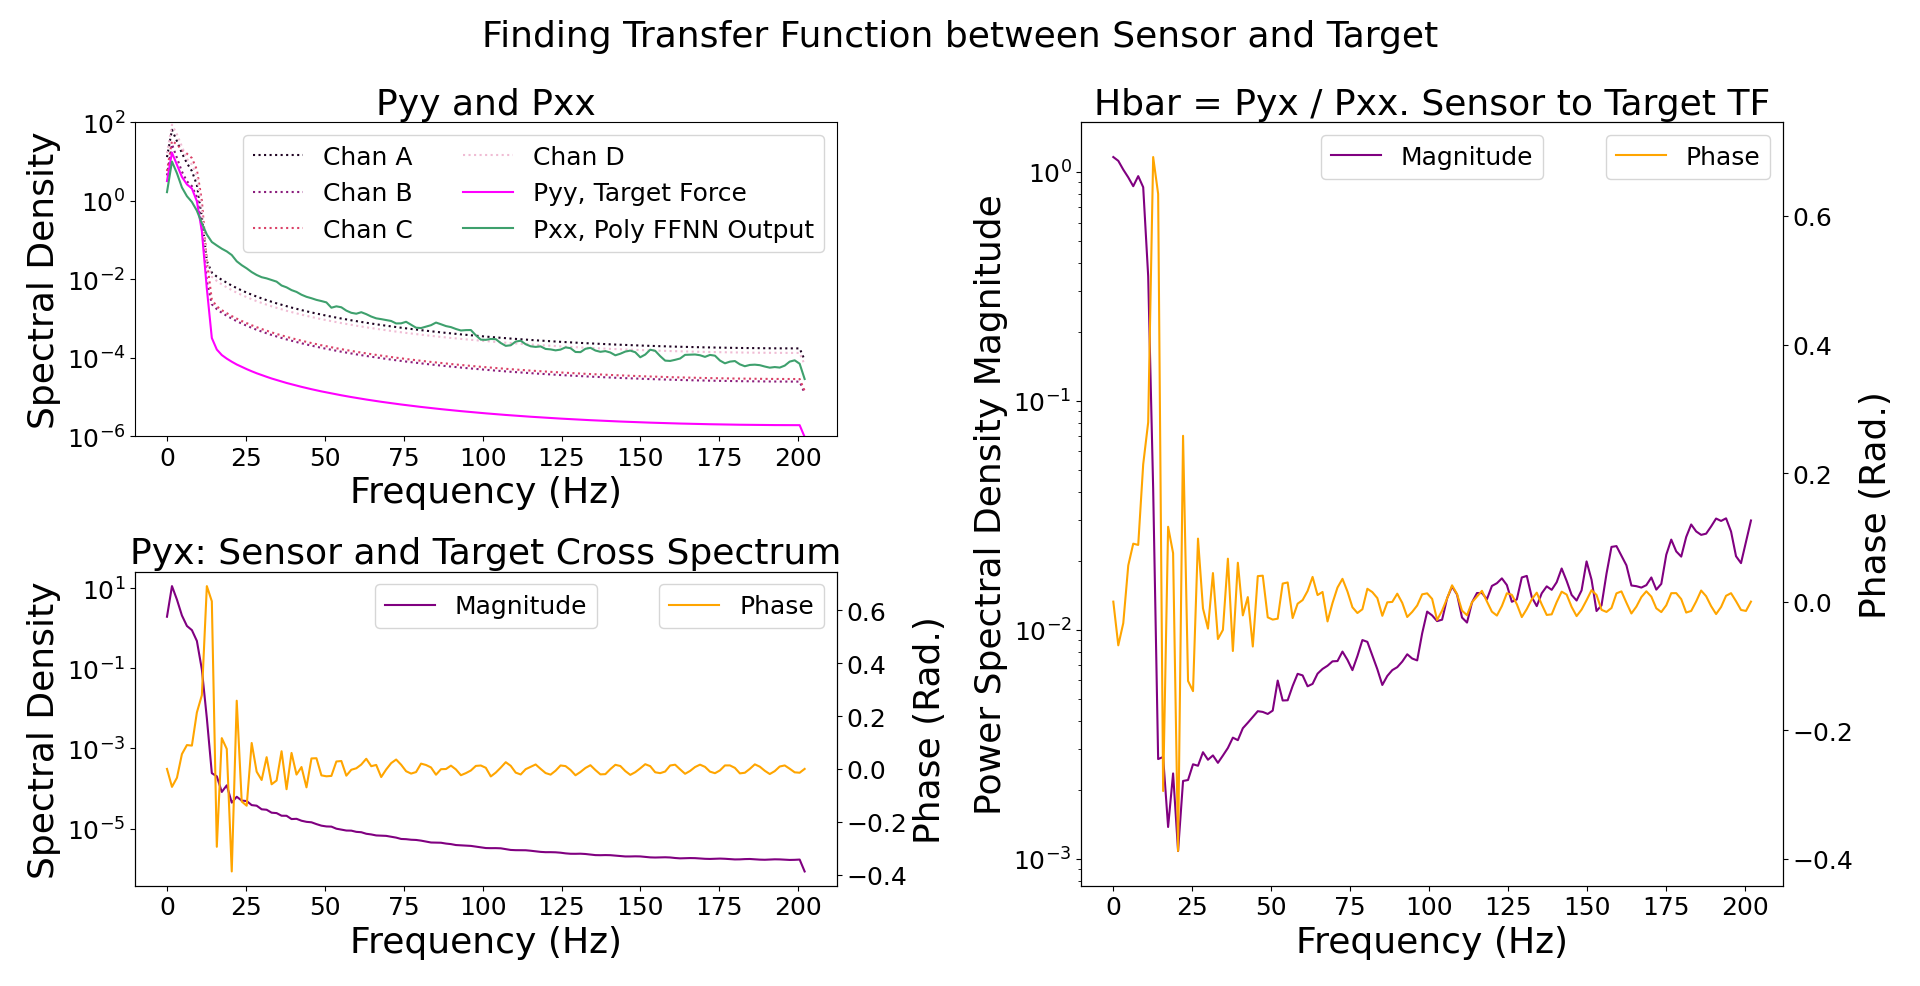
\includegraphics[width=5.5in]{ch10_tf.png}
\caption{
Power spectral density of sensor, target, and transfer function between them.
The regression target has been low pass filtered with a cutoff frequency of 10 Hz,
which can be seen by the steep drop in magnitude at this point.
The individual sensor channels have the same filter applied to limit high frequency input.
The cross spectrum, $P_{yx}$, shows that there is good correlation between the low frequency
components of the estimate and the target.
The transfer function between the estimate and the target suggests that additional 
filtering after the regression method could improve results.
Post-processing requirements depend on the application, and 
additional filtering after regression could be a useful technique for tuning performance.
}
\label{fig:sense_tf}
\end{figure}

\begin{figure}[ht]
\centering
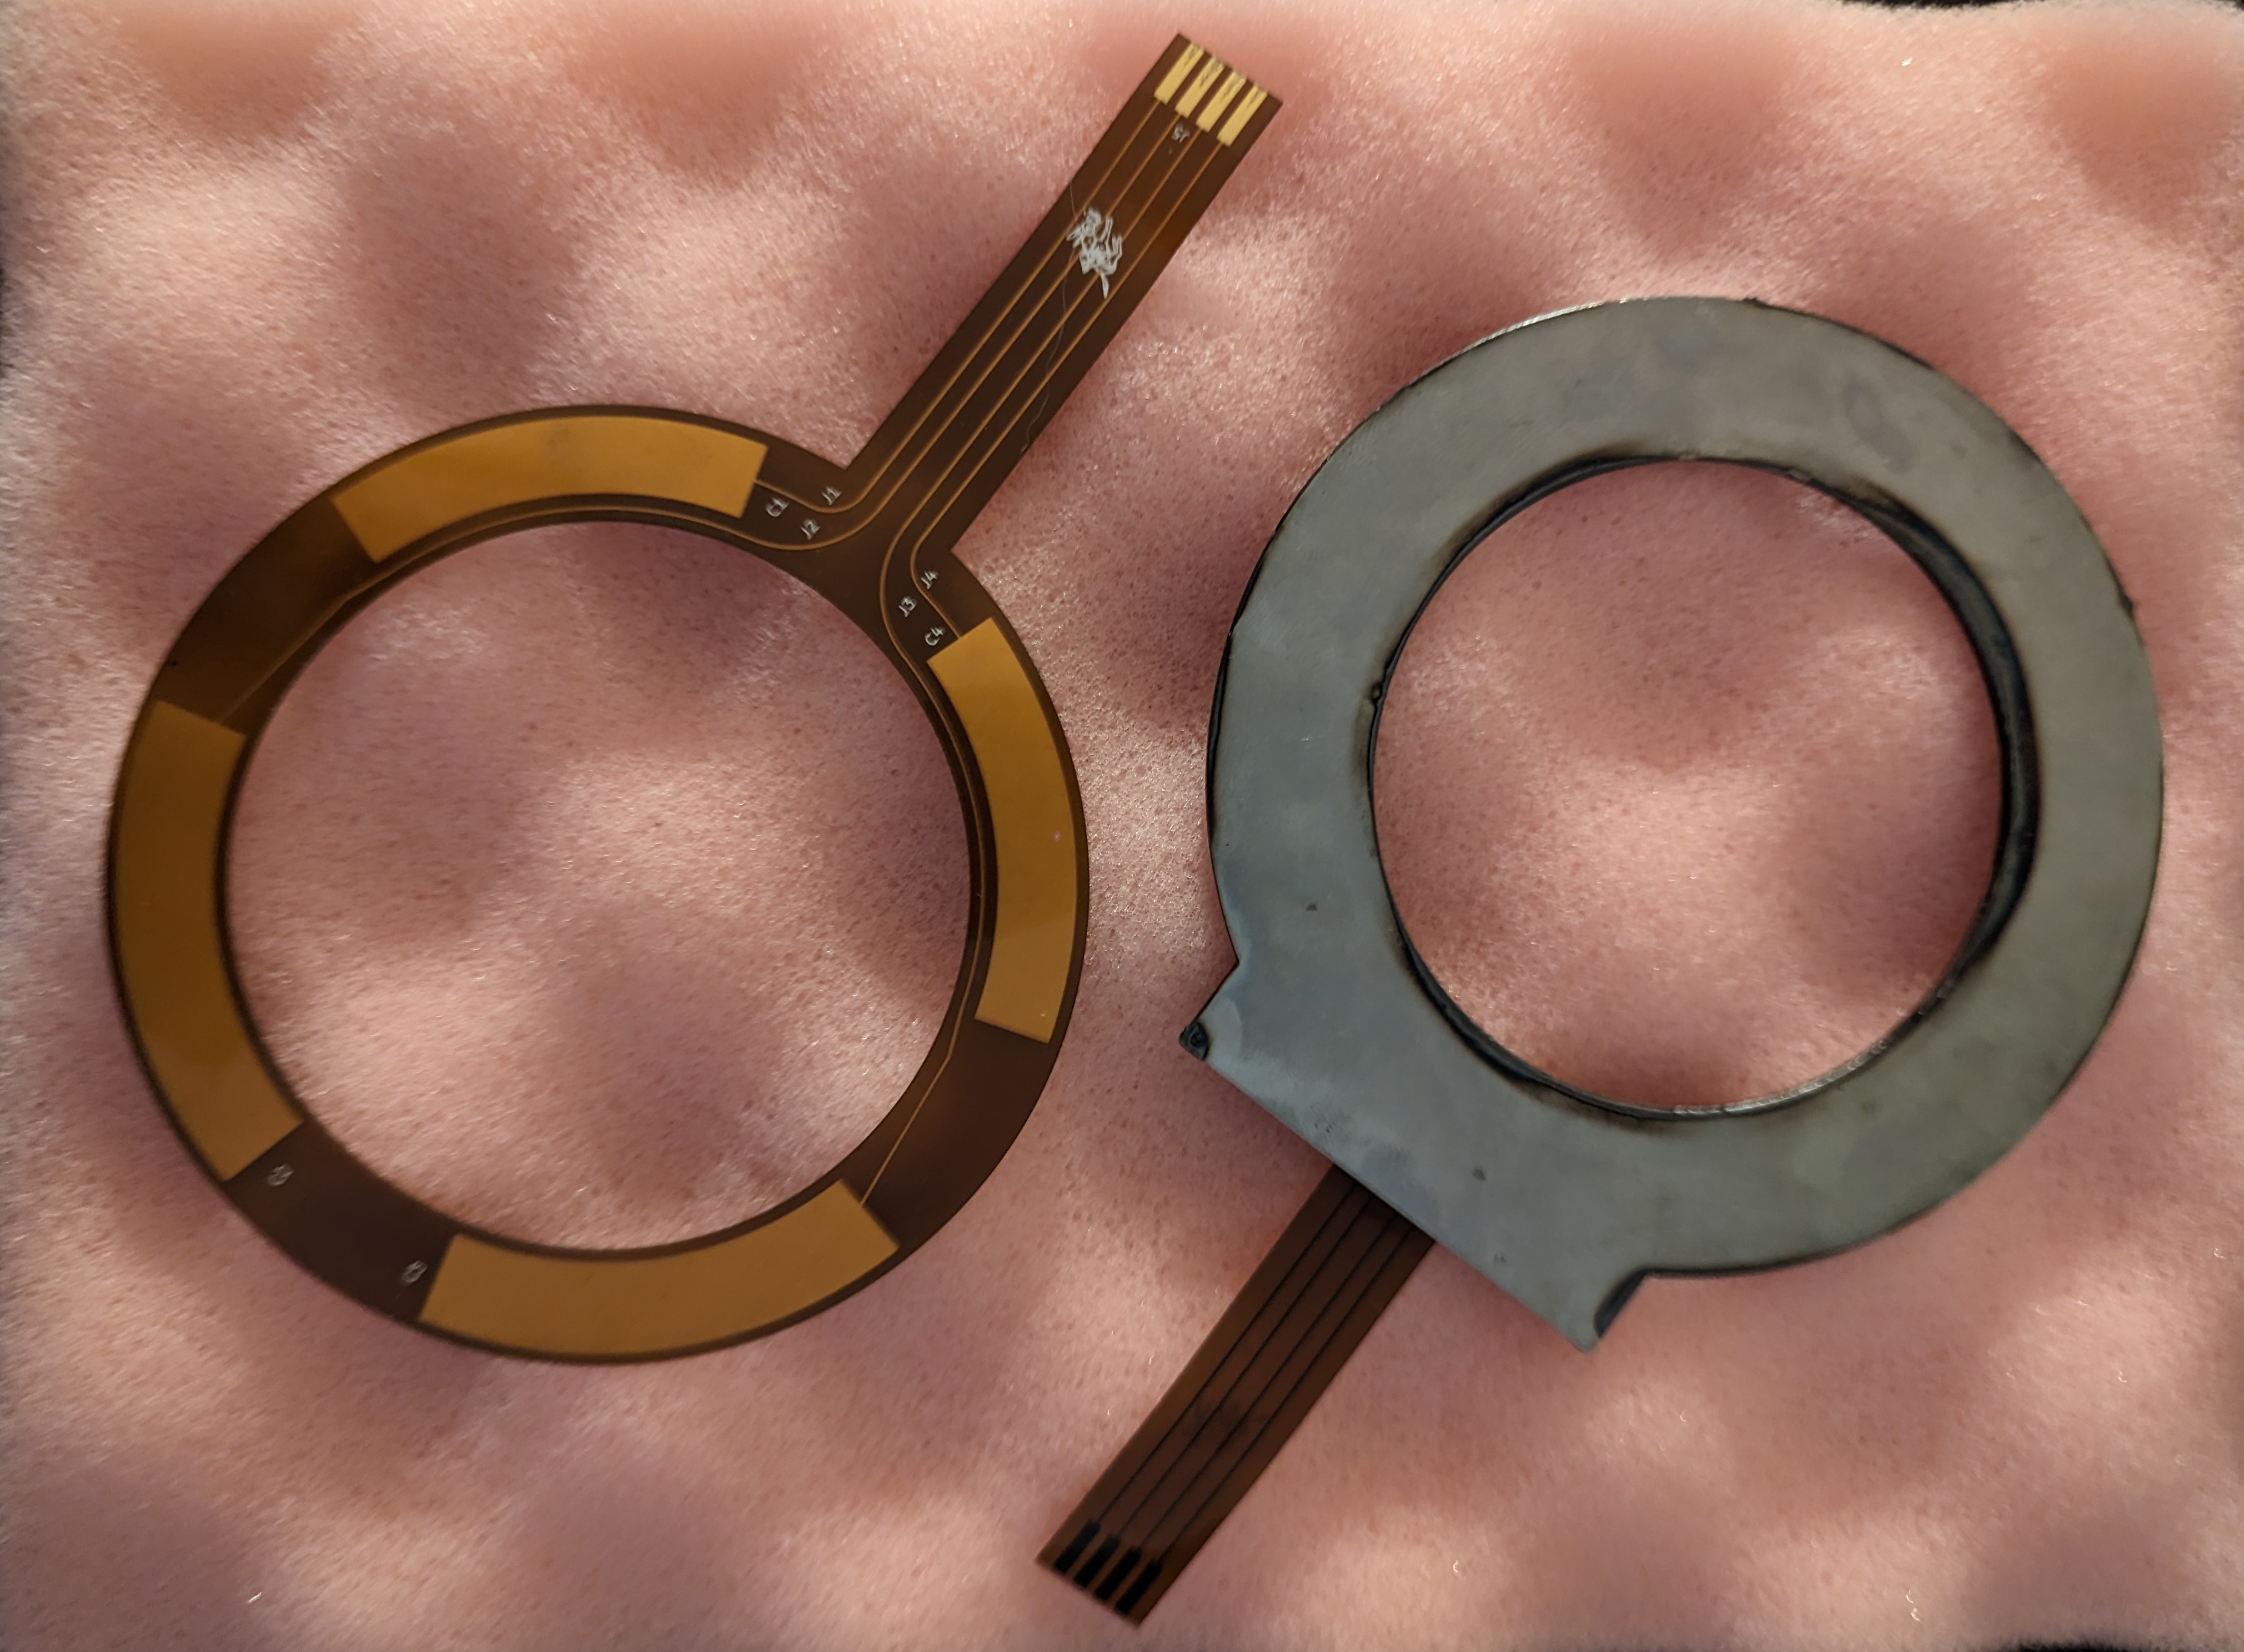
\includegraphics[width=0.5\textwidth]{ch10_airgap_and_case.jpg}
\caption{
The air gap sensor membrane, left, and an assembled prototype, right.
The sensor case provides additional protection from the environment.
The device is assembled via later welding.
Future sensor designs could omit the steel case and integrate the sensor directly within
the block or sleeve of the tool.
This type of sensor measures cutting forces via the change in capacitance caused
by the displacement of the top of the case when force is applied. 
}
\label{fig:airgap}
\end{figure}

 % modelling of sensors expanded, and design improvements

% ><><><><><><><><><><><><><><><><><><><><><><><><><><><><><><><><><><><><><><><><
%                   BACK MATTER: Reference Cited
% ><><><><><><><><><><><><><><><><><><><><><><><><><><><><><><><><><><><><><><><><
\backmatter     % Leave this line here, it sets the formatting requirements for the back matter of the document

% >>>>>>>>> References Cited (required) <<<<<<<<<<
\urlstyle{rm}               % <-- Sets the URL font to be the same as the other text
\bibliography{supporting-files/sources_flexpcb,supporting-files/sn-bibliography,supporting-files/airgap-bibliography,supporting-files/thesis}
%\bibliography{supporting-files/thesis}

% >>>>>>>>> Selected Bibliography (optional) <<<<<<<<<<
%\cleardoublepage
%\begin{selected-bibliography}
%Work Positions

%Review of underground mining technologies

%Review of capacitive sensors

%Constitutive model for materials

%Six axis load cell

%polymide modelling
%<Your selected bibliography would go here, a page break might also be necessary above>
%\end{selected-bibliography}

% Make sure the citations in you .bib file are correct. Especially double check that the resources type is correct. This will dictate how the items in the bibliography are formatted.
% We suggest using a citation management tool to create your .bib file. This make your references machine readable in the click of a button. Attend a Library workshop, visit the Library's website, or speak to a librarian about getting started with a citation management tool. This will make your life much easier. READ: MUCH EASIER! https://libguides.mines.edu/citing/software

% Look at http://bib-it.sourceforge.net/help/fieldsAndEntryTypes.php#phdthesis to find some information on the types of fields that exist. Also recommend using a reference manger. 


% >>>>>>>>> Appendices (if applicable) <<<<<<<<<<
% Laser weld procedure
% Calculation of fringing effects

\appendix{Magical Encoding Awesomeness}\label{app:encoding}
\ref{tab:encoding} shows how several symbols appear in the rendered document.

\begin{table}[H]
	\caption{\label{tab:encoding}This is where we have fun testing encoding}
	\begin{center}
		\begin{tabular}{|c|c|c|}
			\hline
			& Normal & Math \\
			\hline
			The greater than: & > & $>$ \\
			\hline
			The less than: & < & $<$ \\
			\hline
			The tilde: & \textasciitilde{} & $\sim$ \\
			\hline
		\end{tabular}
	\end{center}
\end{table}

\subsection{Test Appendix Sub-Section}\label{sec:longtable}
\ref{tab:longtable} is an example of a very large ``longtable.''
\begin{landscape}
\begin{longtable}{|>{\centering}p{1.02in}|>{\centering}p{1.15in}|>{\centering}p{1in}|>{\centering}p{0.7in}|>{\centering}p{0.7in}|>{\centering}p{0.67in}|>{\centering}p{2.55in}|} %
	\endfirsthead % Remove this line to use the main header for the first page
	\hline%
	Age & Formation  & Thickness (feet)   & Thickness (feet)  & Thickness (feet)  & Aquifer?  & Lithology 	
	\endhead%
	\caption{Stratigraphy of the Granite Mountains and Lost Creek areas\label{tab:longtable}}\\ %
	\hline
	Age & Formation \footnote{Only major unconformities shown, indicated by break in table.} & Thickness (feet) \footnote{Generalized thicknesses from.}  & Thickness (feet) \footnote{Thicknesses shown are approximate and apply to Lost Creek vicinity
	only.} & Thickness (feet) \footnote{Thicknesses shown are from a public screened dataset of logged formation
	tops from the 12 townships surrounding Lost Creek. } & Aquifer? \footnote{Aquifer designations \textendash{} Lost Creek vicinity only.%
	} & Lithology \tabularnewline
	\hline 
	Quaternary  & Alluvium & - & 0-20 & - & Yes & Sands and clays derived chiefly from the Tertiary formations in the
	area. \tabularnewline
	\hline 
	Paleocene & Fort Union  & up to 3,000 & 4,650 & 6,500? & Yes & Consists of alternating fine to coarse grained sandstone siltstone
	and mudstone. Contains various layers of lignitic coal beds. \tabularnewline
	\hline
	\hline 
	Cretaceous  & Lance  & 1,700 to 2,700 & 2,950 & 4,000? & Yes & Interbedded sandstone, siltstone and mudstone. Gray to brownish gray.
	Locally carbonaceous. Sandstone is white to grayish orange. \tabularnewline
	\hline 
	Cretaceous & Fox Hills  &  & 550 & 1,800? & No & Consists of coarsening upward shale and fine-grained sand with thin
	coal beds near the top. Represents a transition from marine to non-marine
	environment. Grades into Lewis Shale at the base. \tabularnewline
	\hline 
	Cretaceous & Lewis Shale  & 1,250 & 1,200 & 1,050 to 2,000 & No & Interbedded dark-gray and olive-gray shale and olive-gray sandstone. \tabularnewline
	\hline
	\hline 
	Cretaceous & Mesaverde Group  & 0 to 1,000 & 800 & 300 to 500? & No & Gray to dark gray shales with interbedded buff to tan fine to medium
	grained sandstones. \tabularnewline
	\hline 
	Cretaceous & Steele and Niobrara Shales  & Cody Shale 4,500 to 5,000 & 2,000 to 2,500 & 2,400 to 5,000 & No & Steele shale is soft gray marine, Niobrara shale is dark gray and
	contains calcareous zones. \tabularnewline
	\hline 
	Cretaceous & Frontier  & 700 to 900 & 500 to 1,000 & 750 to 1,500 & Yes & Gray sandstone and sandy shale. \tabularnewline
	\hline 
	Cretaceous & Dakota  &  & 300 to 400 &  & Yes & Marine sandstone, tan to buff, fine to medium grained may contain
	carbonaceous shale layer. \tabularnewline
	\hline 
	Jurassic  & Nugget Sandstone  & 400 to 525 & 500 &  & Yes & Grayish to dull red coarse grained cross-bedded quartz sandstone. \tabularnewline
	\hline 
	Triassic  & Chugwater  & 1,275 & 1,500 &  & No & Red shale and siltstone contains gypsum partings near the base. \tabularnewline
	\hline 
	Permian  & Phosphoria  & 275 to 325 & 300 &  & No & Black to dark gray shale, chert and phosphorite. \tabularnewline
	\hline 
	Pennsylvanian  & Tensleep and Amsden and Madison  & 600 to 700 & 750 &  & No & White to gray sandstone containing thin limestone and dolomite partings.
	Red and green shale and dolomite, sandstone near base. \tabularnewline
	\hline 
	Cambrian  & Undifferentiated  & 900 to 1,000 & 1,000 &  & No & Siltstone and quartzite, including Flathead sandstone. \tabularnewline
	\hline
	\hline 
	Precambrian  & Basement  & - & - &  & No & Granites, metamorphic and igneous rocks. \tabularnewline
	\hline
\end{longtable}
\end{landscape}

\begin{landscape}
\begin{longtable}{|c|c|c|c|c|c|c|c|c|c|c|c|}
	\endfirsthead
	\caption{Test of a small longtable on the alternate page.} \\
	\hline
	1 & 2 & 3 & 4 & 5 & 6 & 7 & 8 & 9 & 10 & 11 & 12 \\
	\hline
	A & B & C & D & E & F & G & H & I & J & K & L \\
	\hline
\end{longtable}
\end{landscape}

\subsection{This subsection will follow on a new page that is portrait}
Here it is, just an example

\lipsum[3]

\appendix{Capacitance Simulation}\label{app:sim}

Here we have simulation data for the air gap design.
The electric field over a cross section of the electrode floating in space in the steel case
is shown in \ref{fig:app_sim}. The static field strength is calculated for the 
two positions of the case top at no load and max load conditions. 
The relaxed gap is 457 $\mu$m. 
The inner electrode is 30 $\mu$m, and sits 125 $\mu$m above the case.
The difference in dielectric strength above and below the
electrode is ignored for this simulation. 
For the max load conditions, the total gap is 200 $\mu$m.

The simulation points are chosen from the previous load frame characterization data of the sensor case.
The simulation covers a 0.1 degree chunk of the entire ring sensor.
The results of the simulation indicate that the uncompressed sensor should have a capacitance of 0.7 pf per degree of electrode
and the fully compressed electrode should have a capacitiance of 1.8 pf per degree of electrode.
This suggests the capacitance could change by at least 2.5 times its inital value over the travel of the sensor.

\begin{figure}[ht]
\centering
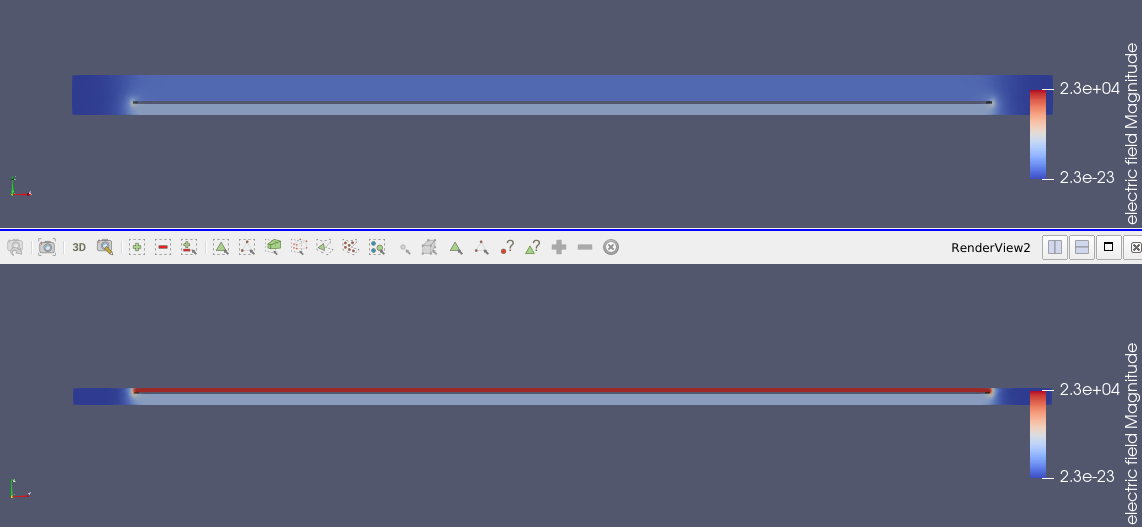
\includegraphics[width=0.7\textwidth]{app_sim.png}
\caption{
Simulation of electric field to determine capacitance properties of air gap design.
The top image shows the relaxed state of the sensor, with low electric field strength 
in the free space around the electrode.
When the air gap compresses, the electric field becomes much stronger and more concentrated,
this is measured as an increase in capacitance. Fringing effects appear to be minimal in this
simulation of the design.
}
\label{fig:app_sim}
\end{figure}


\end{document}
